\documentclass[
    draft=true,
    paper=a4,
    fontsize=11pt,
    twoside=true,
    captions=tableheading,
    british, ngerman,
]{scrreprt}
\usepackage[headsepline]{scrlayer-scrpage}
\pagestyle{scrheadings}
\automark[section]{chapter}

\usepackage{babel}

\usepackage{lipsum}

\usepackage[utf8]{inputenc}
\usepackage[T1]{fontenc}
\usepackage{microtype}

\usepackage{showframe}

\usepackage{newpxtext}
\usepackage{newpxmath}

%\usepackage{float}
\usepackage{booktabs}
\usepackage{amsmath, amssymb}
\usepackage{csquotes}
\usepackage{graphicx}
\usepackage[labelformat=simple]{subcaption}
\renewcommand\thesubfigure{(\alph{subfigure})}

\usepackage{siunitx}
\sisetup{locale = DE}

\usepackage[
    colorlinks=true,
    allcolors=black,
    urlcolor=blue,
]{hyperref}

\setkomafont{captionlabel}{%
    \bfseries
}
\setkomafont{caption}{%
    \bfseries
}
\setcapindent{0em}

\usepackage{listings}
\usepackage{xcolor}
\usepackage[export]{adjustbox}

\definecolor{dark-grey}{rgb}{0.3, 0.3, 0.3}
\definecolor{comment-green}{rgb}{0.0, 0.6, 0.0}

\lstset{
    aboveskip = 1em,
    belowskip = 1em,
%    abovecaptionskip=1em,
    belowcaptionskip=1em,
%    backgroundcolor = \color{black!5},
    basicstyle = \ttfamily,
    caption = \lstname,
    commentstyle = \itshape\color{comment-green},
%     frame = single,
    rulecolor = \color{black!10},
    keywordstyle = \color{blue},
    numbers = left,
    numbersep = 12pt,
    numberstyle = \footnotesize\ttfamily\color{dark-grey},
    stepnumber = 1,
    showstringspaces = false,
    tabsize = 4
}

\usepackage[
    backend = biber, % Sets biber as backend.
    style = authoryear-icomp, % Use [author, year] citing with ibid. when duplicate.
    maxcitenames = 2, % Truncate lists above 2 entries (e.g. names) when citing.
    mincitenames = 1, % Truncate to 1 entry (e.g. names) when citing.
    maxbibnames = 3, % Truncate lists above 3 entries (e.g. names) in bib.
    minbibnames = 3, % Truncate to 3 entries (e.g. names) in bib.
    backref = true, % Show reference to page.
    backrefstyle = three, % Will compress sequences of three pages or mmore, e.g. 1,2,3,5,7 to 1-3,5,7.
    isbn=false,
    url=false, % Note: @Online references will stay unaffected (yay).
    giveninits=true, % Show only initials for given names.
    uniquename=init, % To disable conflict warning because of giveninits.
]{biblatex}
% Space out bib entries a bit.
\setlength\bibitemsep{1.5\itemsep}
% Put lastname before firstname.
\DeclareNameAlias{sortname}{family-given}
% Separates author names with semicolon instead of comma.
\renewcommand{\multinamedelim}{\addsemicolon\space}

% Bib resources.
\addbibresource{../references/references.bib}
\addbibresource{../references/websites.bib}
\addbibresource{../references/unpublished.bib}

\newcommand{\quelle}[1]{{\normalsize \emph{(Quelle: #1)}}}

\newcommand{\quelle}[1]{%
    \mbox{\itshape(Quelle:\ #1)}
}
\newcommand{\wifi}{\mbox{Wi-Fi}}
\newcommand{\unity}[1]{#1}
\newcommand{\imagebox}[1]{%
	{\color{black!25}%
	\framebox[\textwidth]{\normalcolor #1}}%
}


%\includeonly{titlepage, declaration_of_originality, thanks, abstract}

\begin{document}

\pagenumbering{roman}
\begin{titlepage}
	\begin{center}
		\LARGE\textbf{\textsc{Universität Bremen}}\\
		\large\textbf{\textsc{Fachbereich 3: Mathematik/Informatik}}\\
		\vspace{2cm}
		\LARGE \textbf{\textsf{Arbeitstitel}} \\
		\vspace{2cm}
		\LARGE\textbf{\textsc{Masterarbeit}}\\
		\vspace{0.5cm}
		\large
		im Studiengang\\
		\enquote{Informatik Master of Science}\\
		\vspace{1cm}
		\normalsize
		vorgelegt am: \dots \\
		\vspace{3.5cm}
	\end{center}
	\vfill
	\hrule
	\vspace{1em}
	\normalsize{
		\begin{tabular}{ll}
			Name: & {Ralf Manuel Morawe} \\
			Matrikelnummer: & {2615732} \\
			Studiengang: & Informatik\\
			Fachsemester: & 4\\
			Erstgutachter: & {Prof. Dr. Johannes Schöning} \\
			Zweitgutachter: & {\dots} \\
		\end{tabular}\\
	}
\end{titlepage}
\cleardoublepage
\chapter*{Selbstständigkeitserklärung}
\thispagestyle{empty}

Hiermit erkläre ich, dass ich die vorliegende Arbeit selbstständig angefertigt, nicht anderweitig zu Prüfungszwecken vorgelegt und keine anderen als die angegebenen Hilfsmittel verwendet habe. Sämtliche wissentlich verwendete Textausschnitte, Zitate oder Inhalte anderer Verfasser wurden ausdrücklich als solche gekennzeichnet.\\[2ex]
Bremen, den \today\\[6ex]

\begin{tabular}{l}\toprule
	\centering\footnotesize Ralf~Manuel~Morawe
\end{tabular}
\cleardoublepage
%\chapter*{Danksagung}
\thispagestyle{empty}
\lipsum[10-11]
\cleardoublepage
%\chapter*{\abstractname}
\thispagestyle{empty}
\lipsum[1]

\cleardoublepage

\begin{otherlanguage}{british}
\chapter*{\abstractname}
\thispagestyle{empty}

\lipsum[2]

\end{otherlanguage}
\cleardoublepage

\tableofcontents
\cleardoublepage
\pagenumbering{arabic}

\chapter{Einleitung}
\label{chap:einleitung}

Durch den technischen Fortschritt in den letzten Jahren hat sich der Einsatz von \emph{Augmented Reality} (AR) und \emph{Virtual Reality} (VR) in verschiedenen Anwendungsbereichen etabliert \parencite{Krevelen2010, Zhao2009, Sharples2008, Jung2008}.
Als Nutzerschnittstelle dienen dienen in vielen Anwendungen Smartphones, da die Sensoren (Kameras, Gyrosensor etc.) nun ausreichen, um einfache AR-/VR-Inhalte zu präsentieren \parencite{Li2017b,Feng2017,Yoo2015,Mulloni2012}.
Neben Smartphones ermöglichen Head-Mounted Displays (HMDs) die Anzeige von \emph{Mixed-Reality-} (MR) und VR-Inhalten.
Beispielsweise sind hier die \emph{Microsoft HoloLens} \parencite{Microsoft2018} als AR-HMD oder die \emph{Oculus Rift} \parencite{Facebook2018} und \emph{HTC Vive} \parencite{HTCCorporation2018} als VR-HMD zu nennen (siehe \autoref{fig:devices}).
\begin{figure}[hb]
    \centering
    %\imagebox{%
    \begin{minipage}{0.3\textwidth}
        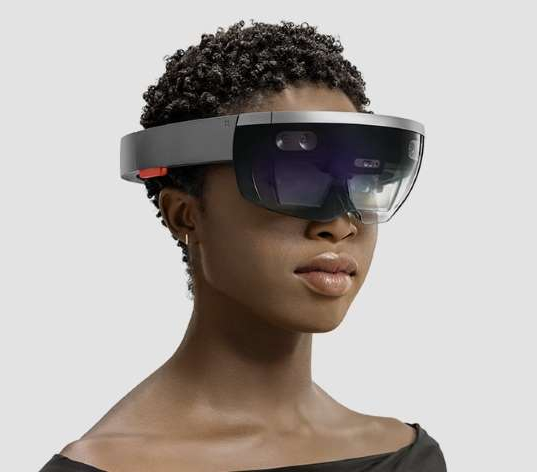
\includegraphics[width=.9\linewidth]{figures/Microsoft2018_HoloLens_worn}
    \end{minipage}%
    \hfill
    \begin{minipage}{0.45\textwidth}
        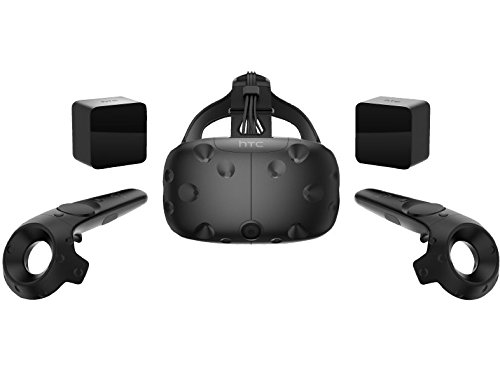
\includegraphics[width=.9\linewidth]{figures/htc_vive}
    \end{minipage}%
    \hfill
    \begin{minipage}{0.25\textwidth}
        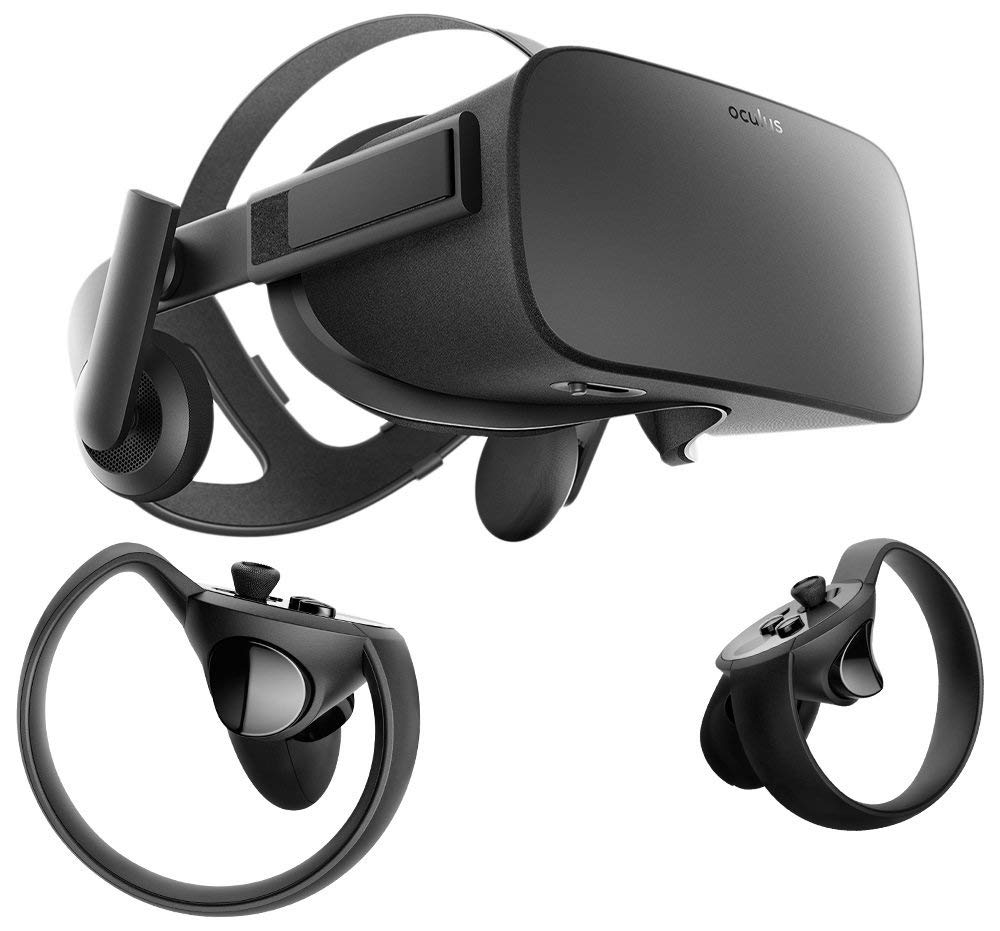
\includegraphics[width=.9\linewidth]{figures/oculus_rift}
    \end{minipage}%
    %}
    \caption{Diverse MR- und VR-HMDs. Microsoft HoloLens (Links), HTC Vive (Mitte) und Oculus Rift (Rechts). \quelle{\cite{Microsoft2018, Amazon2018b, Amazon2018}}}
    \label{fig:devices}
\end{figure}

Bei AR wird die Grenze zwischen dem Reellen und dem Virtuellen aufgehoben, indem virtuelle Inhalte in Echtzeit mit sechs Freiheitsgraden in die reale Welt überlagert werden.
\autoref{fig:mrtouch} zeigt z.B., wie virtuelle Nutzungsschnittstellen in die physische Welt platziert werden und über Berührungsinteraktion gesteuert werden können.
In der Vergangenheit wurde von Forschern AR unter anderem eingesetzt, um räumliche Informationen in der Umgebung von Nutzern anzuzeigen.
Beispielsweise wird die Navigation zwischen zwei Punkten augmentiert.
Die bisherigen Ansätze fokussieren die AR-unterstützte Schritt-für-Schritt-Navigation \parencite{Hoellerer1999, Hashish2017, Mulloni2012} und die Augmentierung von realem Kartenmaterial \parencite{Rohs2009, Morrison2009, Reitmayr2005}.
\begin{figure}[ht]
    \centering
    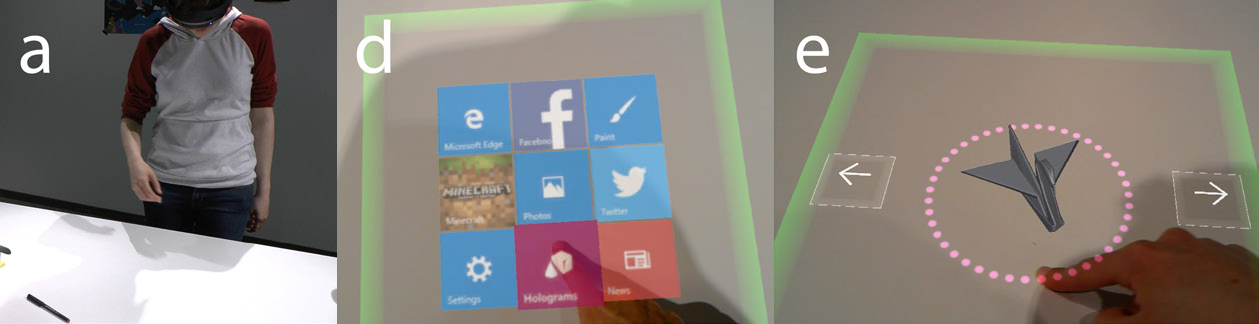
\includegraphics[width=\textwidth]{figures/mrtouch}
    \caption{Virtuelle Interfaces werden auf physischen Oberflächen platziert und mittels Berührungsgesten aktiviert. \quelle{\cite{Xiao2018}}}
    \label{fig:mrtouch}
\end{figure}

\section{Motivation und Ziel der Arbeit}
\label{sec:motivation_ziel}
Das Ziel \emph{dieser} Arbeit ist die Entwicklung einer neuartigen Form, räumliche Informationen mithilfe eines HMDs in eine AR-Szene zu integrieren: die \textbf{Megamap}.
Als Megamap wird in dieser Arbeit einer Kartendarstellung definiert, bei der ein dreidimensionales Abbild der Umgebung um den Nutzer herum gezeigt wird.
Die Karte ist in einem verkleinerten Maßstab zur Umgebung und ist in diese verankert.
Das bedeutet, wenn sich der Nutzer in der Welt bewegt, dann bewegt er sich auch auf der Karte.
Die virtuelle Karte verhält sich somit, als sei sie ein reales Objekt in der Umgebung.

Die ursprüngliche Idee für die Megamap-Darstellung stammt aus dem Spiel \emph{Tom Clancy's The Division} (TCTD) \parencite{Ubisoft2018} (siehe \autoref{fig:megamap}).
Eine Karte der Umgebung (eine Variante von New York) wird mit relevanten Spielobjekten und Ortsnamen \emph{im Spiel} als AR-Interface um den Charakter herum angezeigt.
Die Karte erlaubt dem Spieler unter anderem, Wegpunkte festzulegen (Navigation), interessante Punkte in der Umgebung anzuzeigen und zu filtern (Exploration) sowie die Ansicht durch Verschieben und Zoomen der Karte anzupassen.
Ebenso werden Missionsziele, andere Charaktere und Events durch Icons in der Karte hervorgehoben.
All diese Informationen sind vom aktuellen Kontext des Spiels abhängig.
Das heißt, es werden nur Informationen angezeigt die für die aktuelle Spielsituation des Spielers relevant sind.
\begin{figure}[t]
    \centering
    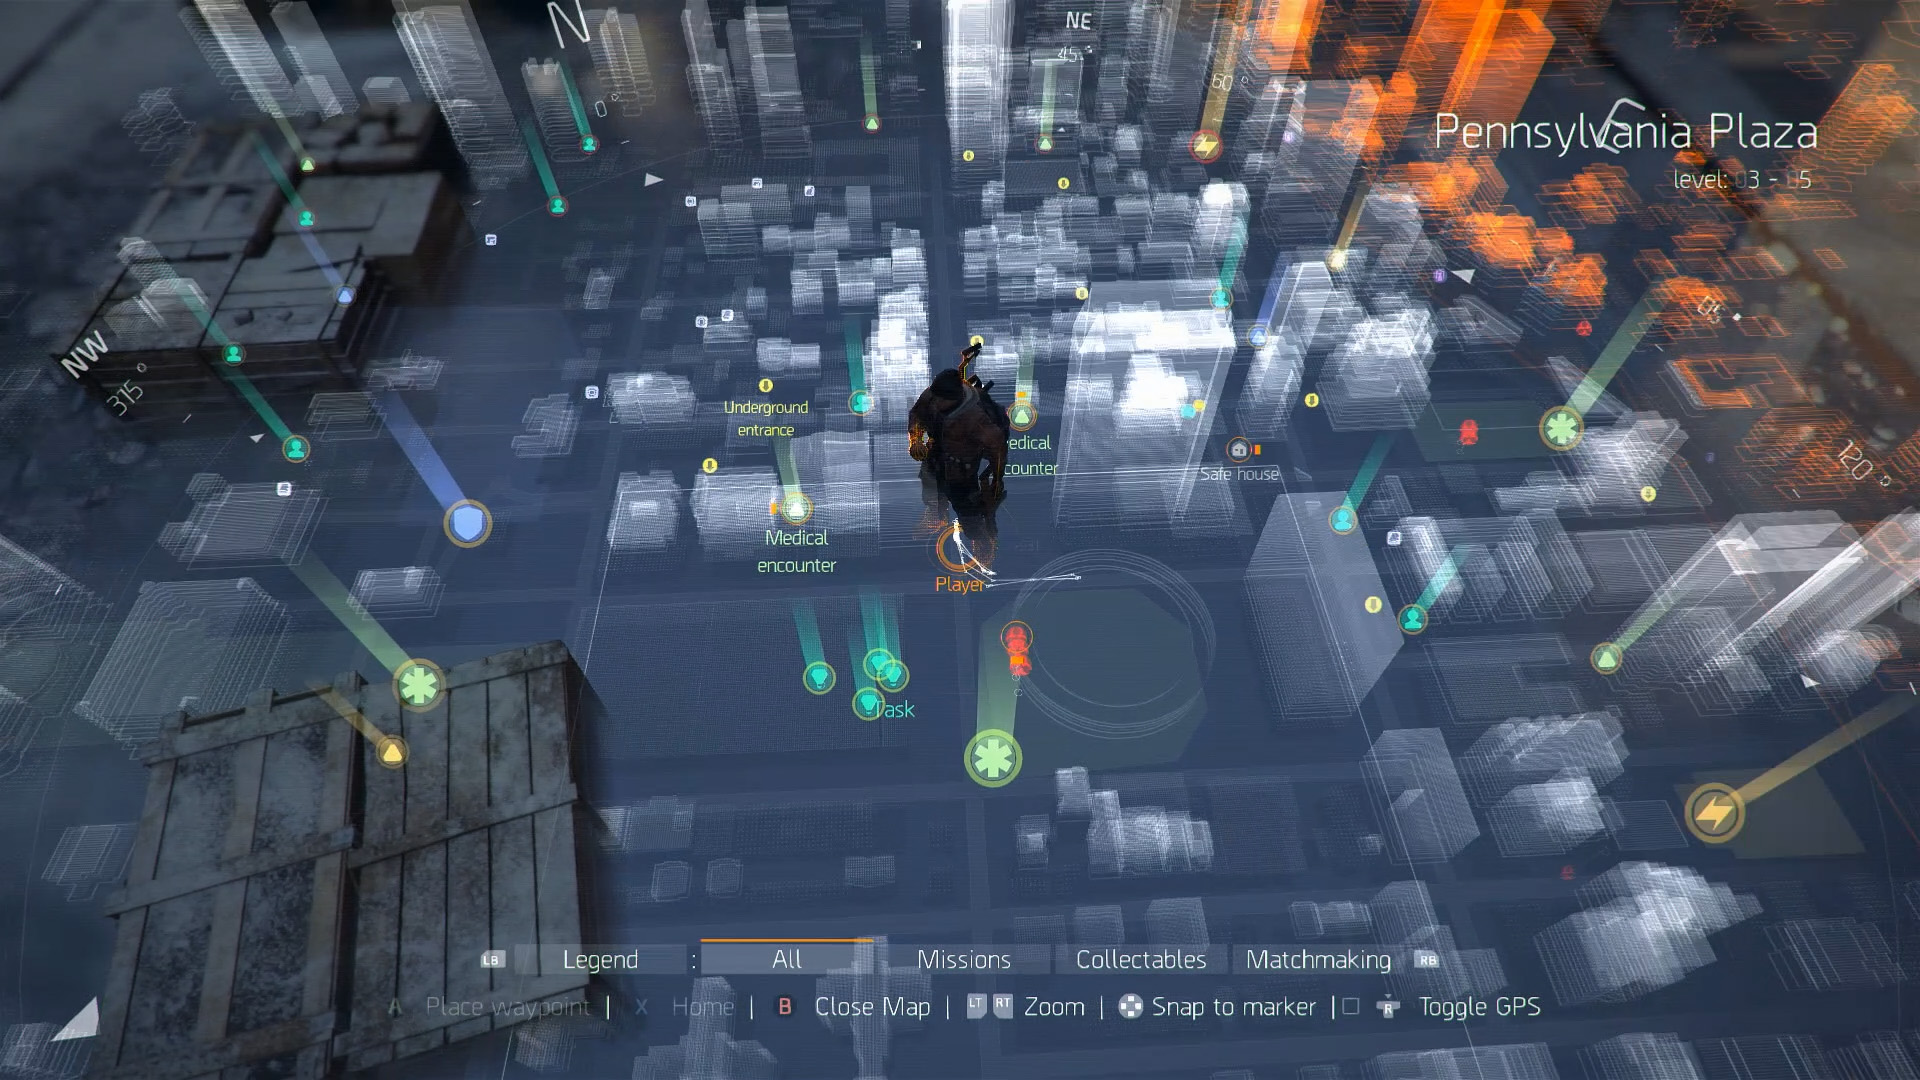
\includegraphics[width=\textwidth]{figures/the_division_megamap.jpg}
    \caption{Die \enquote{Megamap} aus \emph{Tom Clancy's The Division}. Symbole zeigen Missionsziele, Gegenstände und wichtige Orte im Spiel. \quelle{\cite{MYDIVISION.NET2014}}}
    \label{fig:megamap}
\end{figure}

%Eine Kartendarstellung existiert in dieser Form bisher nur im Spiel.
%In der realen Welt werden Karten zwar zunehmend durch AR/VR unterstützt.
%Eine Anwendung wie die Megamap aus TCTD, bei der die Karte in die Umgebung integriert ist, gibt es bisher aber noch nicht.
%Dafür gibt es mehrere Gründe:
%\begin{enumerate}
%    \item Die bisherigen Lösungen zur AR-unterstützten Kartenexploration stützen sich meistens auf die Überlagerung von virtuellen Information auf physische Objekte, beispielsweise eine reale Karte.
%    Dabei wird häufig ein Smartphone als \emph{Magic Lens} (\enquote{Magische Lupe},~\cite{Bier1994}) eingesetzt, auf dem die virtuellen Informationen vor dem Hintergrund der Kamera angezeigt werden.
%    Solch ein Ansatz ist jedoch nur Bedingt für den mobilen Einsatz geeignet.
%    Einem Fußgänger würde das gleichzeitige Halten einer Karte und eines Smartphones schwerfallen, besonders während des Laufens.
%    Auch der Einsatz eines Projektors, der die Informationen auf eine Karte projiziert, ist hierfür nicht geeignet.
%
%    \item Die durch virtuelle Helfer unterstützte Navigation ist ein Ansatz, der sich in der Forschung häufig finden lässt.
%    Allerdings ist die reine Navigation nicht der einzige Anwendungsfall in Bezug auf Kartenanwendungen.
%    Wie \textcite{Reichenbacher2001} detailliert beschreibt gibt es weitere Anwendungsfälle, die sich unter dem Oberbegriff der \emph{Kartenexploration} zusammenfassen lassen.
%    Darin eingeschlossen sind zum Beispiel die zuvor erwähnten Szenarios der Restaurantsuche oder der Anzeige von Fahrt- oder Öffnungszeiten.
%    Allgemein gesagt geht es bei der Kartenexploration um die \enquote{Entdeckung} von Orten anhand von Karten.
%    Diese Anwendungsfälle werden jedoch, in Bezug auf Unterstützung durch AR/VR, seltener behandelt als die Unterstützung der reinen Navigation.
%
%    \item Die Ansätze in der Literatur nutzen in der Regel Smartphones oder andere Handgeräte.
%    Obwohl die Entwicklung dieser Geräte technologisch rasch voranschreitet, sind sie auf die Möglichkeiten der Kamera-Bildsensoren, Gyrosensoren und GPS-Sensoren beschränkt.
%    Z.B. ist die dreidimensionale Rekonstruktion einer Szene, wenn überhaupt, nur sehr vereinfacht möglich.
%\end{enumerate}
%
%Die Integration der Karte in die Umgebung wäre jedoch von Vorteil.
%Denn eine von der Umgebung getrennte virtuelle Karte, wie es bei vielen aktuellen Smartphone-Anwendungen der Fall ist, kann die Aufmerksamkeit des Nutzers von der eigentlichen Umgebung ablenken.
%Die Nutzer müssen ständig das virtuelle Bild mit ihrer Umgebung abgleichen.
%Dies ist nicht nur ein zusätzlicher mentaler Aufwand.
%Im schlimmsten Fall kann es zu schweren Unfällen kommen wenn die Nutzer auf die virtuelle Darstellung achten oder die dargestellten Informationen beim Abgleich mit der Umgebung fehlinterpretieren \parencites{Medenica2011}{Lin2017}.
%
%Weitere Schwierigkeiten ergeben sich bei der Darstellung von \emph{Indoor}-Karten (Karten von Gebäuden).
%Die Überlagerung von mehreren Stockwerken stellt ebenso ein Problem dar wie die Tatsache, dass das GPS innerhalb von Gebäuden nicht verfügbar ist.
%Daher setzen sich viele existierende Ansätze mit der Navigation oder Lokalisierung innerhalb von Gebäuden auseinander.
%Der Anwendungsfall der Karten\emph{exploration} von Gebäuden wird hingegen bisher wenig behandelt.
%Weil kaum öffentliche Gebäudedaten verfügbar sind (im Gegensatz zu \emph{Outdoor}-Daten wie z.B. von \emph{Open Street Map} \parencite{OpenStreetMapFoundation2018}) wird die Situation weiter erschwert.

Eine Darstellung von räumlichen Informationen als Megamap bietet gegenüber herkömmlichen Ansätzen einige Vorteile:
\begin{itemize}
    \item Durch die Verwendung des HMDs bleiben die Hände der Nutzer frei. %
    Sie können die Karte nutzen und gleichzeitig mit beiden Händen mit der Umgebung interagieren.

    \item Da die Kartenansicht in die Umgebung der Nutzer integriert ist, müssen Nutzer die Kartendarstellung mit der Umgebung nicht wiederholt abgleichen. %
    So wird der Umgebung genug Aufmerksamkeit geschenkt und der mentale Aufwand der Nutzung wird verringert \parencite{Bark2014, Narzt2006, Kim2009}.

    \item Dadurch, dass die Karte in die Umgebung verankert ist und sich mit ihr mitbewegt, kann die Megamap auch während der Fortbewegung genutzt werden.

    \item Mit der Megamap können sowohl Außen- als auch Innenbereiche (z.B. Gebäude) dargestellt werden.
\end{itemize}

Die Recherche des Verfassers ergab keine Anwendungen, die das zuvor beschriebene Konzept einer Megamap umsetzen.
Daher wird im Rahmen dieser Arbeit eine Megamap-Anwendung entwickelt.
Spezifisch zielt die Anwendung auf die Nutzung in Innenbereichen wie Gebäude ab, da bisherige MR-HMDs Probleme mit der Verwendung im Freien aufweisen \parencite{Schroeder2017, Strange2018}.

Da sich außerdem die bisherigen Ansätze mit der Karten\emph{navigation} (\enquote{von A nach B}) beschäftigen, wird in dieser Masterarbeit der Anwendungsfall der Karten\emph{exploration} fokussiert.
Bei der Kartenexploration geht es um die Erkundung von Umgebungen anhand von kontextbasierten Ortsdaten.
Kontextbasierte Ortsdaten sind Daten, die von der aktuellen Situation abhängig sind, wie z.B. der aktuellen Position des Nutzers (\textquote{Wo ist das von mir aus nächste Restaurant?}/\textquote{Wieviele Spielplätze sind in meiner Nähe?}).
Ortsdaten können ebenso von der Zeit abhängen (\textquote{Welche Supermärkte in der Gegend sind geöffnet?}).
Übertragen auf die Innenbereichsnutzung stehen mit der Megamap verschiedene explorative Funktionen bereit, beispielsweise das Suchen nach den Büros von Personen oder den Standorten von öffentlichen Druckern.
Nutzer können sich mit der Megamap einen detaillierten Überblick über das Gebäude verschaffen, in dem sie sich befinden.

Als Zielplattform dient das Vive-HMD.
HMDs haben gegenüber Smartphones einige technische Vorteile.
Positionen und Orientierungen der Nutzer sind über Tracking präziser möglich.
MR-HMDs wie die HoloLens oder die \emph{Magic Leap One} \parencite[siehe \autoref{fig:magic_leap}]{MagicLeap2018} verwenden Infrarotkameras, um Strukturen der Umgebung virtuell in Echzeit zu rekonstruieren.
Die reale Umgebung bleibt dank des durchsichtigen Glases weiterhin sichtbar.
Zudem können die Hände für Gesteninteraktionen oder Kontroller verwendet werden anstatt das Display halten zu müssen.
\begin{figure}[tb]
    \centering
    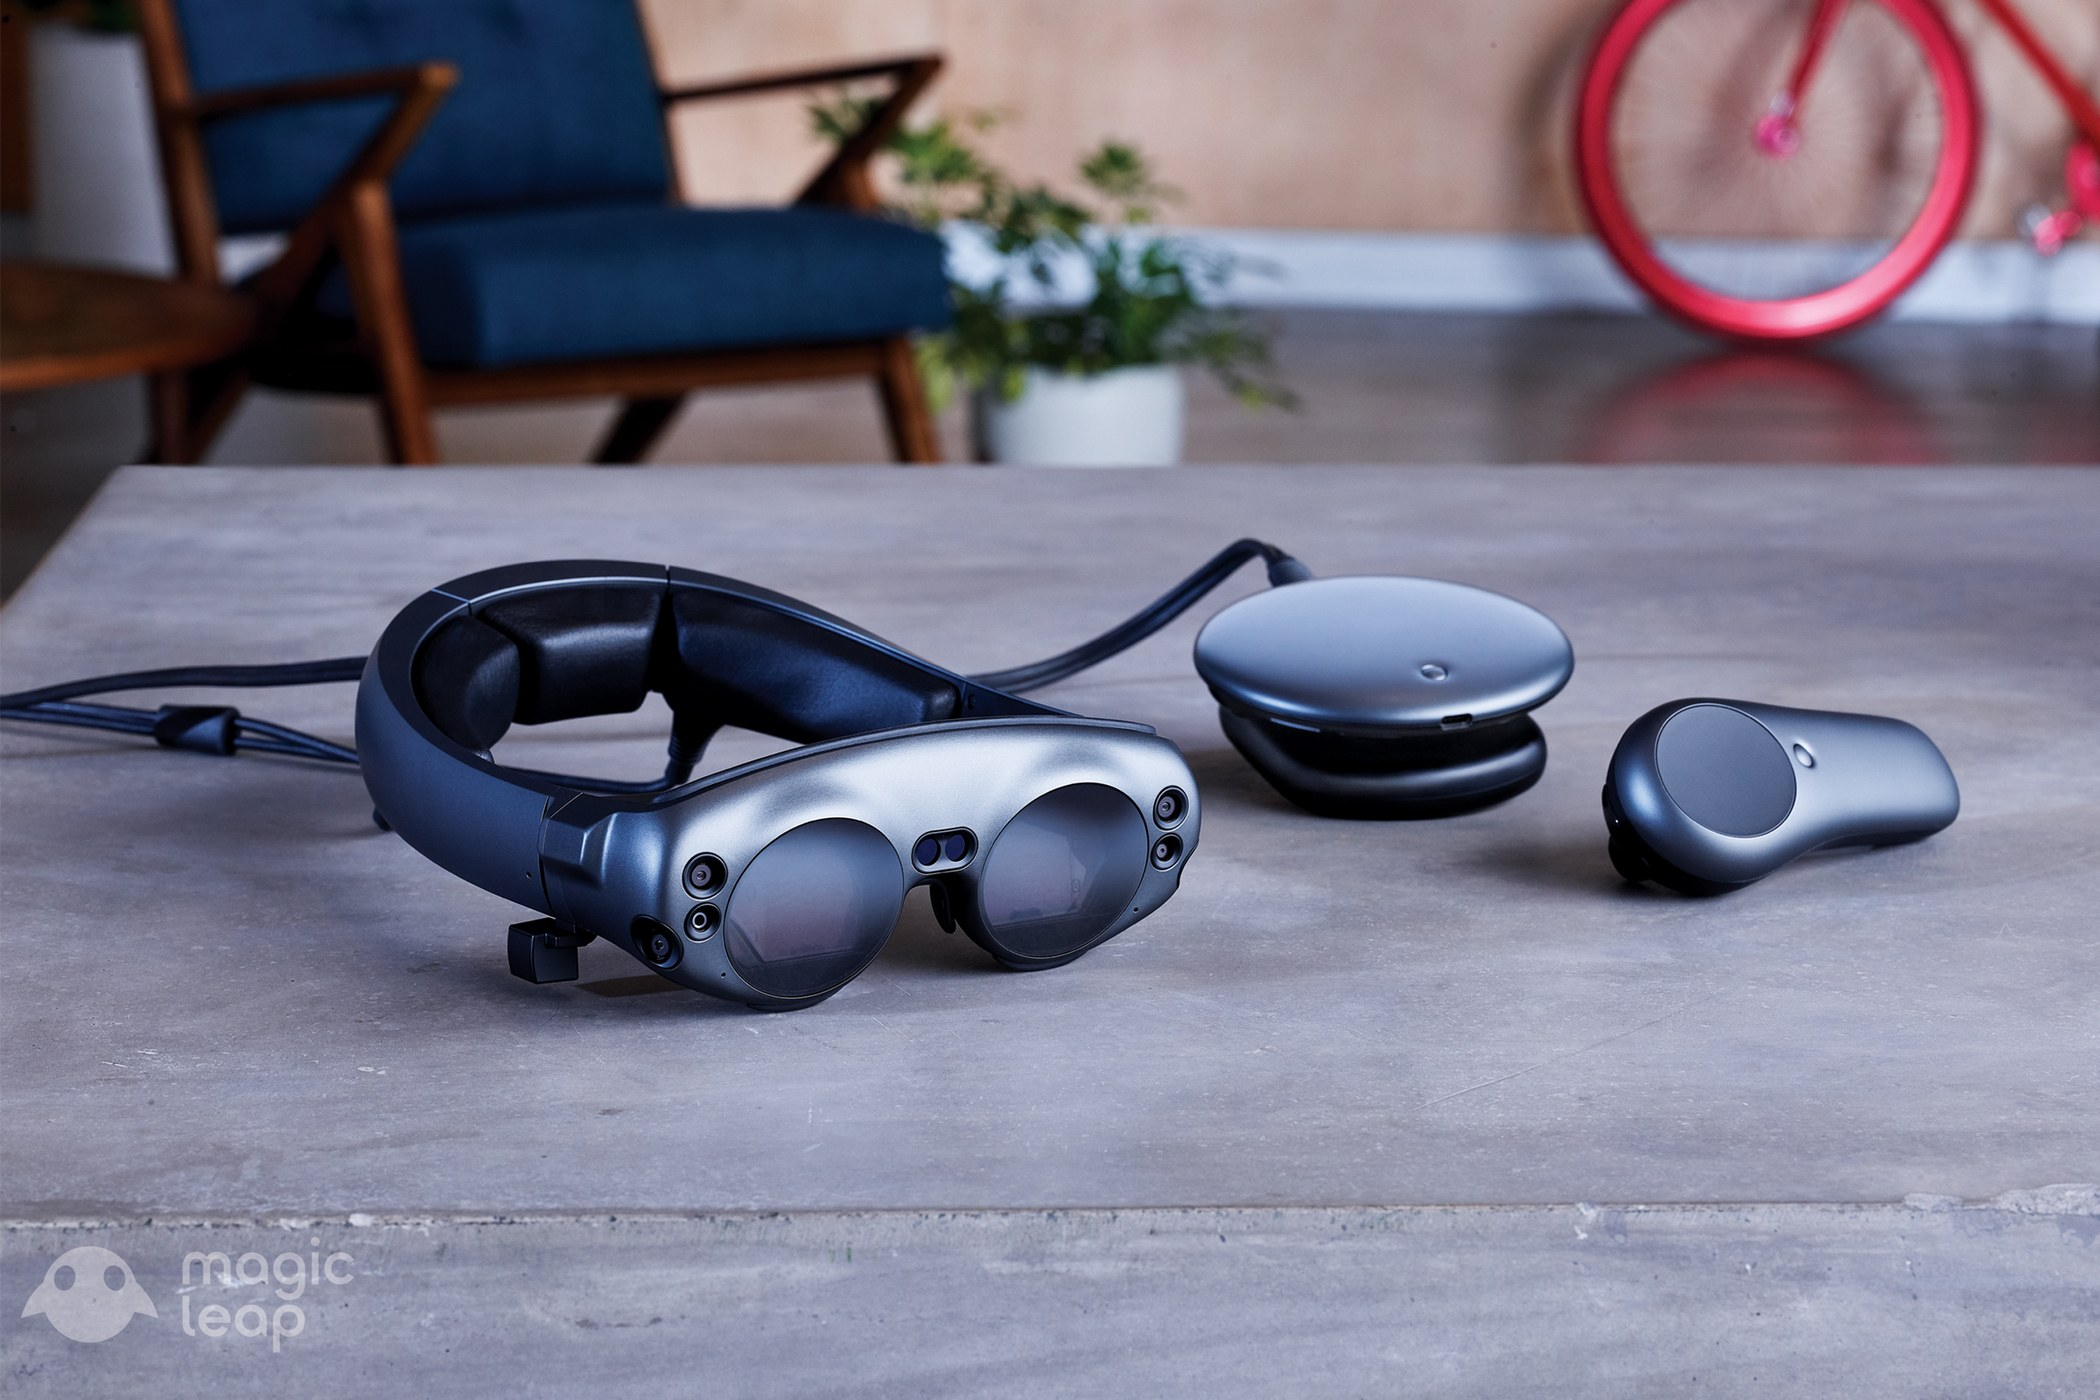
\includegraphics[trim={0, 7cm, 0, 7cm}, clip, width=\textwidth]{figures/magicleap}
    \caption{Das Magic Leap One MR-HMD. \quelle{\cite{MagicLeap2018b}}}
    \label{fig:magic_leap}
\end{figure}

Zu Beginn der Arbeit war das Ziel die Implementierung der Megamap für das Magic Leap One HMD.
Da dieses aber erst im späteren Verlauf der Arbeit veröffentlich wurde, wurde stattdessen die Implementierung für das Vive-HMD in VR umgesetzt.
Die \enquote{reale} Umgebung des Nutzers wird dabei virtuell nachgebildet.
Dadurch lässt sich die Megamap-Anwendung in zukünftigen Arbeiten auf ein MR-HMD übertragen.

%Die Implementierung der Megamap dient der Beantwortung der zentralen Fragestellung dieser Arbeit:
%\begin{quote}
%    \itshape
%    Ist eine in die Umgebung integrierte 3D-Megamap geeignet, um Nutzer bei der Exploration von Gebäuden zu unterstützen?
%\end{quote}
%Der Prototyp wird daher in einer Nutztungsevaluation getestet, um seine Effektivität für die Gebäudeexploration festzustellen.

%Als Inspirationsquelle für die Anwendung dienen neben bereits existierenden Kartenanwendungen wie Google Maps und Ansätzen aus der Forschung auch digitale Spiele.
%Da in Spielen Aufgaben wie Navigation und Exploration von großer Bedeutung sind, kann hier unterschiedliche Ansätze zur Navigations- und Explorationsunterstützung gefunden werden.
%Dies ist am Beispiel TCTD erkennbar.

Da die Idee für die Megamap einem Videospiel entspringt ist nicht unmittelbar klar, ob sich das Konzept auf die Nutzung in der realen Welt übertragen lässt.
Insbesondere, weil die Megamap aus TCTDs Dritte-Person-Perspektive (\emph{Third-Person Perspective}) in die Egoperspektive überführt wird.
Die Eignung der Megamap für die Kartenexploration wird daher am entwickelten Prototypen in einer Nutzerstudie überprüft.
Einerseits werden die subjektiven Eindrücke der Probanden von der Nutzung der Megamap festgehalten.
Andererseits wird die Performance im Vergleich zu einer herkömmlichen 2D-Darstellung einer Indoor-Karte verglichen.

\section{Struktur der Arbeit}
\label{sec:struktur}
Die restliche Arbeit ist in die folgenden Abschnitte unterteilt:

\noindent
Im nächsten Kapitel wird der Stand der Forschung und Technik zur Darstellung von dreidimensionalen Karten beleuchtet.
Die Unterschiede zum Konzept dieser Arbeit sowie deren Beitrag zum Thema werden ebenso herausgearbeitet.
\autoref{chap:concept} geht detailliert auf die Konzeptionierung der 3D-Megamap ein.
Es wird vor allem beschrieben, welche Interaktionen für die Kartenexploration wichtig sind und wie diese in der Megamap-Anwendung umgesetzt werden sollen.
Danach wird in \autoref{chap:implementation} die Implementierung der Anwendung beschrieben.
Ebenso werden Probleme bei der Implementierung erläutert, die für zukünftige Arbeiten beachtet werden sollten.
\autoref{chap:evaluation} präsentiert die Durchführung der Nutzungsevaluation der Anwendung sowie deren Ergebnisse.
Schließlich werden in \autoref{chap:closing} offene Fragen und Probleme dieser Arbeit genannt, welche für zukünftige Arbeiten von Interesse sind.
%
\cleardoublepage

\chapter{Stand der Forschung}
\label{chap:related_work}

\section{Von Realität bis Virtualität}
Da es sich bei den unten genannten Arbeiten und Systeme um AR-/VR-Anwendungen handelt, müssen vorab die Unterschiede zu herkömmlichen Computerprogrammen und mobilen Applikationen geklärt werden.
Im Folgenden werden die Begriffe \emph{Augmented/Virtual Reality} definiert und ein Überblick der wichtigsten Technologien wird gegeben.

\textcite{Milgram1994} stellen das Konzept eines Kontinuums von Realität zur Virtualität vor (siehe \autoref{fig:rv_kontinuum}).
Anwendungen und Technologien lassen sich dabei in dieses Kontinuum einordnen.
Allgemein werden dabei die Kategorien Augmented Reality, Augmented Virtuality und Virtual Reality unterschieden.

\begin{figure}[h]
    \centering
    \imageframe{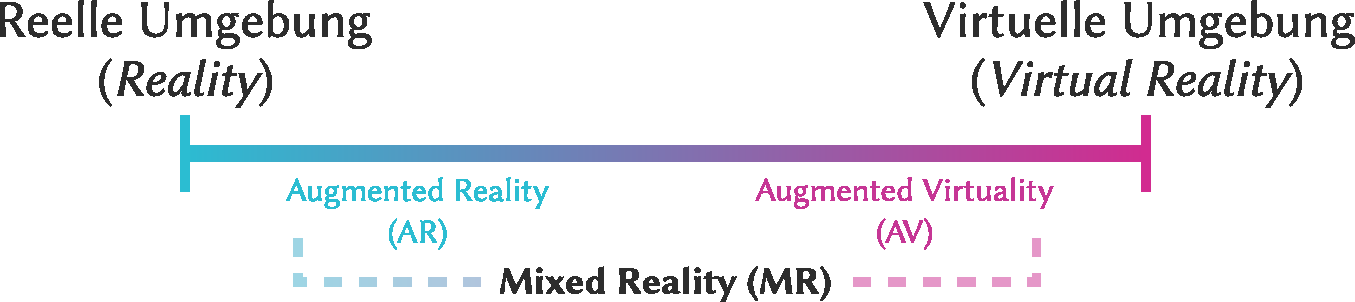
\includegraphics[width=0.9\linewidth]{figures/rv_kontinuum_milgram.pdf}}
    \caption{Das Realität-Virtualität-Kontinuum nach \textcite{Milgram1994}. Je nach Anwendung wird die Realität mehr und mehr mit virtuellen Objekten überlagert, bis schließlich nur noch eine virtuelle Umgebung dargestellt wird.}
    \label{fig:rv_kontinuum}
\end{figure}

Nach \textcite{Azuma1997} bezeichnet \emph{Augmented Reality} Systeme, welche die folgenden Eigenschaften besitzen:
\begin{itemize}
    \item Reale und virtuelle Inhalte werden kombiniert. Häufig werden hierfür virtuelle Objekte auf die reale Umgebung überlagert.
    \item Der Nutzer kann in Echtzeit mit den Systemen interagieren. So zählen z.B. Spezialeffekte in Filmen \emph{nicht} als AR.
    \item Die Inhalte werden dreidimensional mit der Umgebung registriert. Demnach ist ein 2D-Interface vor einer realen Umgebung \emph{kein} AR, selbst wenn es interaktiv ist.
\end{itemize}
AR selbst lässt sich dabei noch in die Kategorien \emph{Spatial AR} und \emph{See-Through AR} einteilen.
Bei Spatial AR werden digitale Informationen direkt in die Umgebung des Nutzers projiziert, z.B. mit einem Projektor auf einen Tisch.
Beim See-Through AR hingegen werden Displays genutzt, die entweder ein Live-Video der Umgebung zeigen oder aber transparent und damit durchsichtig sind.
Dies können See-Through HMDs wie die Microsoft HoloLens sein, aber auch Smartphones in einer entsprechenden HMD-Halterung, bei denen die Rückseitenkamera für ein Live-Bild der Umgebung genutzt wird.
Hier werden die virtuellen Informationen direkt auf dem Display überlagert \autocite{Zachmann2015}.

Bei der \emph{Augmented Virtuality} (AV) werden umgekehrt reale Informationen in eine virtuelle Umgebung eingebettet.
Als Beispiel nennt \textcite[6]{Schroeder2017} die Wetterkarte im Fernsehen, bei der eine \emph{virtuelle} Karte \emph{reale} Wetterinformationen darstellt und um einen \emph{realen} Moderator erweitert wird.
Es sei darauf hingewiesen, dass in diesem Beispiel die Interaktion zwischen dem Moderator und der Karte besteht, nicht etwa zwischen dem Zuschauer und der Karte.

\emph{Virtual Reality} ist die Bezeichnung für Anwendungen, die sich komplett in einer virtuellen Umgebung abspielen.
Um VR von herkömmlichen Computersimulationen abzugrenzen nennt \textcite{Zachmann2015} die intuitive Echtzeit-Interaktion als ein wichtiges Kriterium.
Dabei können Nutzer mit der virtuellen Umgebung über Eingabegeräte wie z.B. Controller mit sechs Freiheitsgraden (6DOF) oder haptischen Eingabegeräten interagieren.
Ein weiteres wichtiges Kriterium ist die Immersion.
Diese ergibt sich aus der Summe der vom System stimulierten und gleichzeitig abgeschirmten Sinne.
Aus diesem Grund werden bei VR-Anwendungen häufig HMDs eingesetzt, da diese gleichzeitig den Sehsinn vor der Außenwelt abschirmen und mit virtuellen Bildern stimulieren können.
% TODO: Links zu den Displayarten.
Aber auch halb-immersive Displays wie eine \emph{Cave}, eine \emph{Powerwall} oder ein Volumendisplay sind möglich.

\textcite{Milgram1994} nennen ebenfalls den Begriff der \emph{Mixed Reality} (MR).
Dieser wird in der Literatur als Oberbegriff sowohl für AR als auch AV verwendet.
Der Begriff hebt die Kombination von realen und virtuellen Inhalten hervor.

\section{Augmentierte Navigation}
Bereits \textcite{Hoellerer1999} stellen ein AR-System vor, bei dem zwei Nutzer kooperieren können.
Der eine Nutzer bewegt sich zu Fuß mit einem HMD und einem Tablet-Computer in der Außenwelt.
Durch das HMD können ihm augmentierte Informationen zur Umgebung und sogar ganze virtuelle Gebäude dargestellt werden, die mit der Umgebung registriert sind.
Der andere Nutzer kann entweder über ein Desktop-Interface oder eine AR-Darstellung der Karte Routen und Informationen in der Umgebung platzieren.
Damit stellt diese Arbeit eine frühe Implementierung für ein HMD dar, die sowohl Navigations- als auch Explorationsaufgaben unterstützt.

Wie bereits in \autoref{sec:motivation_ziel} erwähnt fokussiert sich ein großer Teil der bisherigen Forschung auf den Usecase der Navigation von einem Punkt zu einem anderen.
Vor allem das AR-unterstützte Autofahren wird betrachtet, da hier eine fehlerfreie Navigation wichtig ist und im Fehlerfall sogar fatale Folgen haben kann \parencite{Lin2017}.
Ein häufig eingesetztes Mittel ist hier die virtuelle Hervorhebung der Straßenführung.
\textcite{Narzt2006} präsentieren ein allgemeines Framework zur Darstellung einer virtuellen Route.
Das Framwork kann sowohl für Fahrzeug- als auch Fußgängernavigation und auf verschiedenen Endgeräten eingesetzt werden.
Für den Einsatz im Auto schlagen die Autoren die Windschutzscheibe als Display vor.
Dadurch wäre das AR-Display in der natürlichen Umgebung des Nutzers integriert.
\textcite{Bark2014} erweitern diesen Ansatz.
Sie ersetzen in einem zuvor aufgenommenen Video die statische virtuelle Route durch eine Reihe animierter Papierflieger, die entlang der geplanten Route fliegen.
\textcite{Kim2009} ersetzen die Route sogar durch eine 2.5D-Karte mithilfe eines Fahrsimulators.
Von der Oberseite der Windschutzscheibe schiebt sich eine 2D-Karte ins Sichtfeld, die sich nach und nach dreidimensional mit der Straße verbindet.
Bei beiden Ansätzen wiesen die Autoren beim Vergleich mit einem herkömmlichen \emph{top-down} GPS-System nach, dass die Probanden dem Straßenverlauf durch die AR-Unterstützung besser folgen konnten und weniger Fehler bei der Navigation machten.

\textcite{Alnabhan2014} präsentieren einen Ansatz zur \emph{Indoor}-Navigation als \emph{Android-App}.
Die App nutzt \emph{\wifi-Fingerprinting} und den digitalen Kompass eines Smartphones/Tablets zur Positionierung und Orientierung.
Über vordefinierte Referenzpunkte im Gebäude wird die Ungenauigkeit des \wifi-Fingerprintings ausgeglichen.
Navigationshinweise werden als AR-Pfeil angezeigt (mit zusätzlichen Textausgaben).
Alternativ dazu zeigen \textcite{Liu2016} einen ähnlichen Ansatz, bei dem die Positionierung jedoch auf Magnetfeldsensoren aufbaut und daher weder auf GPS noch auf Infrastruktur wie \wifi oder Marker angewiesen ist.
% TODO: Diesen Satz anpassen, je nachdem wie die Entwicklung der Megamap ausgeht.
Das zeigt, dass AR-unterstützte Kartenanwendungen durchaus auch innerhalb von Gebäuden umsetzbar sind.

\section{Digitale Kartenexploration}
Zur AR-Exploration tragen \textcite{Reitmayr2005} bei, indem sie eine reale Papierkarte durch einen Projektor augmentieren.
\autoref{fig:reitmayr2005_helicopter_map} zeigt die Funktionsweise.
Ein projizierter Helikopter kann mit einem realen \emph{Personal Digital Assistant} (PDA) bewegt werden, wenn dieser in die Nähe gehalten wird.
Der PDA zeigt währenddessen ein Interface zur Kontrolle des Helikopters.
Der Helikopter dient als Cursor für kontextbasierte Informationen.
Sobald der Nutzer einen Rahmen auf die Karte legt, projiziert der Projektor ein Bild der aktuellen Kartenposition aus ungefährer Sicht des Helikopters auf ihn.
Zudem kann der Zustand der Karte durch die Projektion dynamisch verändert werden (in diesem Fall werden Gezeiten von Gewässern simuliert).
Auch wenn diese Arbeit nicht für einen mobilen Einsatz geeignet ist, wird deutlich, dass mit AR nicht nur ortsbezogene sondern auch zeitbezogene Daten auf einer Karte dargestellt werden können.
Dies erlaubt also zusätzlich eine Exploration in der zeitlichen Dimension einer Karte.

\begin{figure}[h]
    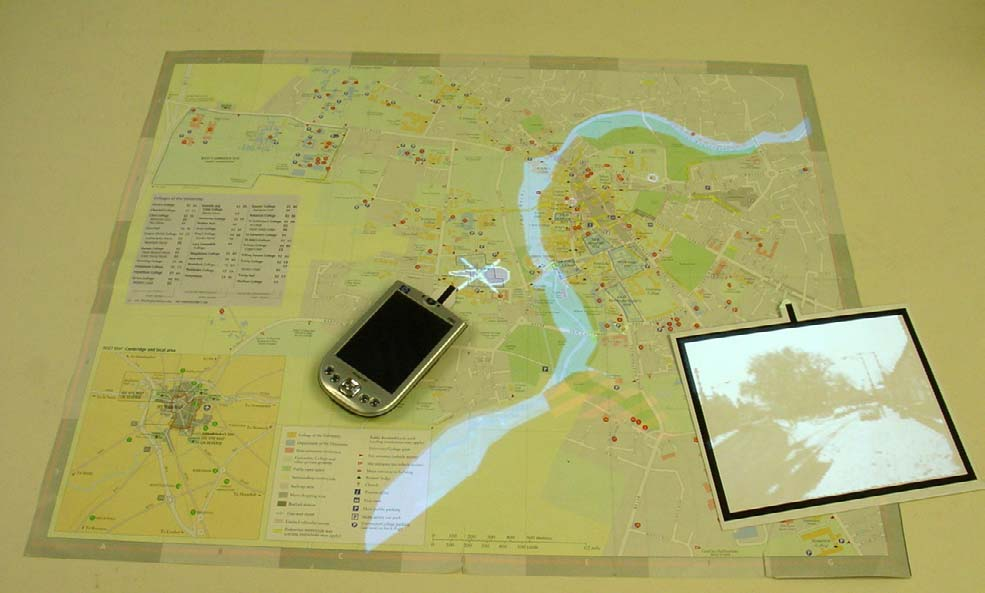
\includegraphics[width=\textwidth]{figures/reitmayr2005_helicopter_map.png}
    \caption{Eine reale Papierkarte wird durch einen Projektor mit virtuellen Inhalten angereichert. \quelle{\cite{Reitmayr2005}}}
    \label{fig:reitmayr2005_helicopter_map}
\end{figure}

\section{Virtuelle Umgebungen als World-in-Miniature}
% WIM
Die Idee der Megamap ist im Prinzip, ein herunterskaliertes Abbild der Umgebung um den Nutzer zu platzieren.
Damit ist die Megamap eine Variante der World-in-Miniature-Metapher (WIM).
Dies ist ein Ansatz zur Unterstützung von Navigation und Interaktion, der vor allem in virtuellen Welten Anwendung findet.
Dabei wird die nähere Umgebung miniaturisiert dargestellt und häufig als eigenständiges Objekt vom Nutzer in der Hand gehalten.
Je nach Anwendung ergeben sich hieraus unterschiedliche Interaktionsmöglichkeiten \parencite{Stoakley1995}.

\textcites{Mulloni2011a}{Mulloni2012} nutzen einen kombinierten Ansatz aus AR-Hinweisen und WIM.\@
Während Nutzer durch ein Gebäude navigieren werden AR-Pfeile sowie Navigationsanweisungen in Form von \enquote{Aktivitäten} auf einem Smartphone angezeigt (\autoref{sfig:mulloni2011_wim_b}, \subref{sfig:mulloni2011_wim_e}).
Sobald zuvor platzierte Poster an Infopunkten im Gebäude erreicht und gescannt werden, wechselt die Ansicht zu einer WIM-Darstellung der Etage mit der hervorgehobenen Route zum Zielort (\autoref{sfig:mulloni2011_wim_a}, \subref{sfig:mulloni2011_wim_c}, \subref{sfig:mulloni2011_wim_d}).
Laut dem Ergebnis der Studie der Autoren hilft die WIM-Übersicht den Nutzern, gewisse Orientierungspunkte (\emph{\enquote{Landmarks}}) in der Umgebung wiederzuerkennen, was zu weniger Fehlern bei der Navigation führt.
Von diesem Aspekt könnte auch die Megamap profitieren, welche eine WIM-ähnliche Sicht der näheren Umgebung liefert.

\begin{figure}[h]
    \begin{subfigure}{.195\textwidth}
        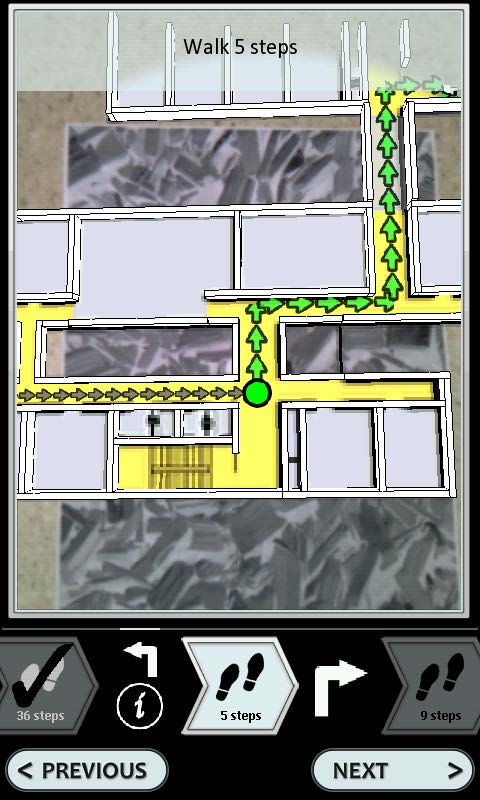
\includegraphics[width=\textwidth]{figures/mulloni2011_wim_a.png}
        \caption{}
        \label{sfig:mulloni2011_wim_a}
    \end{subfigure}
    \hfill
    \begin{subfigure}{.195\textwidth}
        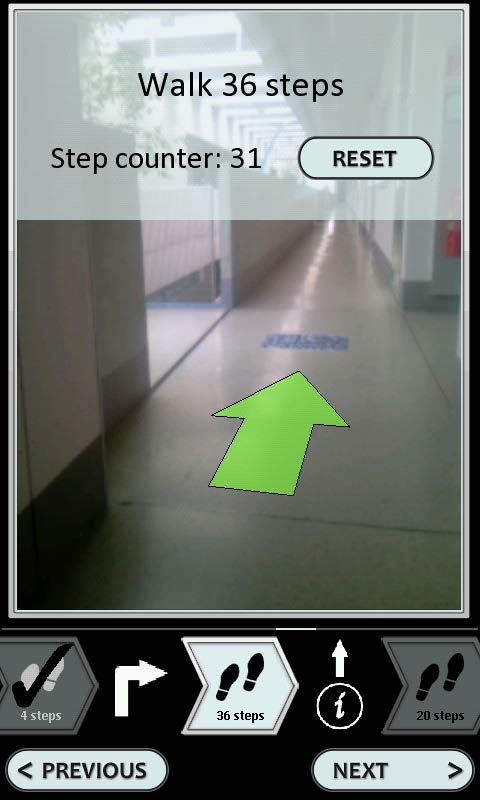
\includegraphics[width=\textwidth]{figures/mulloni2011_wim_b.png}
        \caption{}
        \label{sfig:mulloni2011_wim_b}
    \end{subfigure}
    \hfill
    \begin{subfigure}{.195\textwidth}
        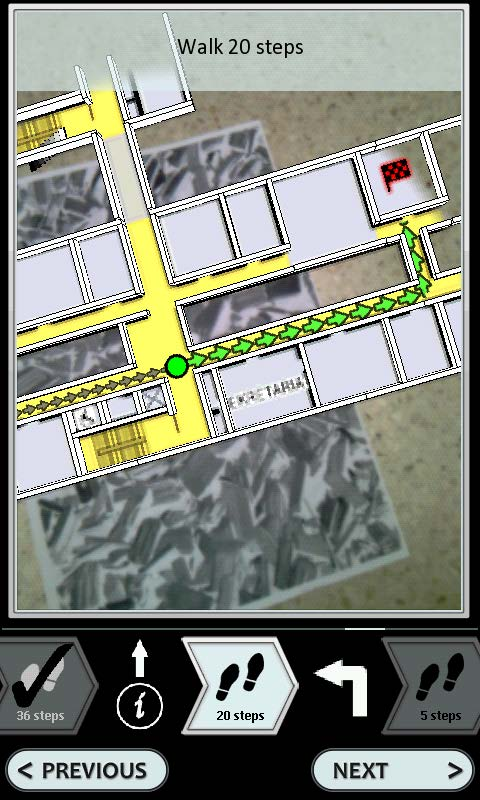
\includegraphics[width=\textwidth]{figures/mulloni2011_wim_c.png}
        \caption{}
        \label{sfig:mulloni2011_wim_c}
    \end{subfigure}
    \hfill
    \begin{subfigure}{.195\textwidth}
        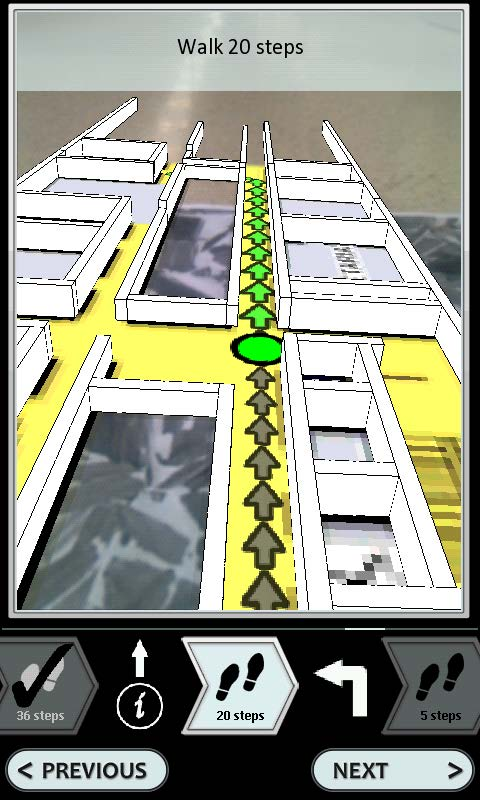
\includegraphics[width=\textwidth]{figures/mulloni2011_wim_d.png}
        \caption{}
        \label{sfig:mulloni2011_wim_d}
    \end{subfigure}
    \hfill
    \begin{subfigure}{.195\textwidth}
        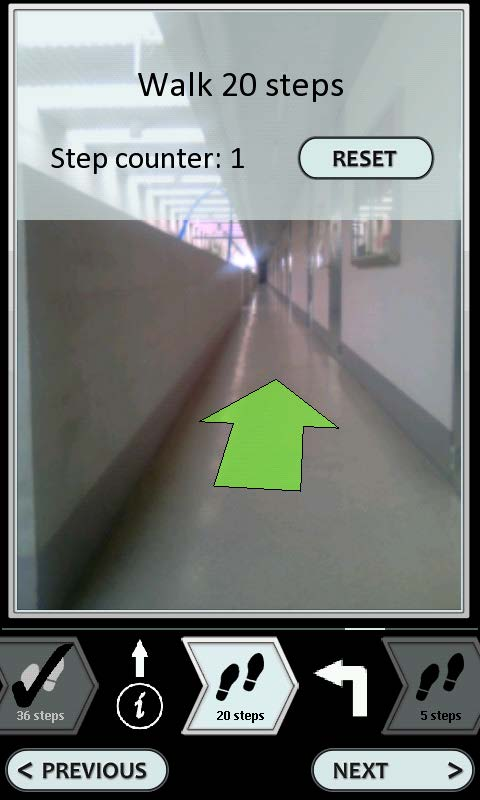
\includegraphics[width=\textwidth]{figures/mulloni2011_wim_e.png}
        \caption{}
        \label{sfig:mulloni2011_wim_e}
    \end{subfigure}
    \caption{AR-Interface für Indoor-Navigation basierend auf WIM.\@ An den Lokalisierungspunkten wird die Indoor-Karte als WIM angezeigt und mit der Position/Rotation der Umgebung registriert. \quelle{\cite{Mulloni2011}}}
    \label{fig:mulloni2011_wim}
\end{figure}

\textcite{Chittaro2005} erweitern das Konzept von WIM für mehrstöckige Gebäude als eine \emph{BreakAway}-Karte (\autoref{fig:chittaro2005_breakaway}).
Hier können einzelne Stockwerke zur Seite geschoben und ausgeblendet werden, um so auf Stockwerke blicken zu können, auf denen sich der Nutzer selbst gar nicht befindet.
Dies erleichtert die Exploration von Gebäuden, da diese schneller nach den gewünschten Eigenschaften durchsucht werden können.

\begin{figure}[h]
    \begin{subfigure}{.49\textwidth}
        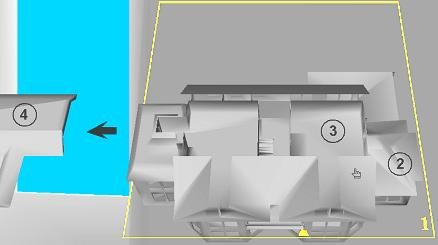
\includegraphics[width=\textwidth]{figures/chittaro2005_breakaway_a.png}
%        \caption{}
    \end{subfigure}
    \hfill
    \begin{subfigure}{.49\textwidth}
        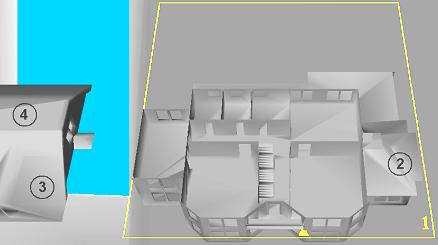
\includegraphics[width=\textwidth]{figures/chittaro2005_breakaway_b.png}
%        \caption{}
    \end{subfigure}
    \caption{In der \emph{\enquote{Examine View}} der BreakAway-Karte können Stockwerke zur Seite geschoben werden, um den Blick auf darunterliegende Stockwerke zu ermöglichen. \quelle{\cite{Chittaro2005}}}
    \label{fig:chittaro2005_breakaway}
\end{figure}

\textcite{Vallance2001} schlagen zudem eine Krümmung der WIM-Umgebung vor, um so eine Verdeckung durch Wände und andere Objekte zu minimieren.

\section{Kartenexploration in digitalen Spielen}
% TODO Übergang?
Im Bereich der Video- und Computerspiele untersuchen \textcites{Moura2014}{Moura2015} den Zusammenhang zwischen eingesetzten Navigationshelfern, Design der Level, sowie Spielmechaniken zur Unterstützung der Navigation.
Daraus leiten \textcite{Moura2015} eine Klassifikation von Navigationshelfern ab.
Außerdem erstellen sie eine Liste von Design-Richtlinien, welche die Vor- und Nachteile der jeweiligen Helfer erläutern und als Hilfestellung für Entwicklung von neuen Spielen dienen.
Diese Designrichtlinien werden in die Entwicklung der Megamap mit einbezogen.

Aufbauend auf die Navigationshelfer in Spielen untersucht \textcite{Lodts2015}, ob diese Helfer auch in der realen Welt anwendbar sind.
Dazu wurden unterschiedliche Helfer, wie sie aus Spielen bekannt sind, für das \emph{Google Glass} implementiert.
In einem Test, aufgeteilt in die Aufgabenbereiche Navigation, Orientierung, Exploration und Annotation, wurde ermittelt welche der Helfer den Nutzern bei der jeweiligen Aufgabe am hilfreichsten sind.
Es zeigt sich, dass Helfer, die in der Umgebung eingebettet sind (z.B. AR-Pfeile oder -Text, farbliche Hervorhebungen von Objekten) effektiver sind als statische Anzeigen per \emph{Head-Up Display} (HUD).
Daher wird bei der Entwicklung der Megamap-Anwendung der AR-Darstellung von Inhalten mehr Beachtung geschenkt.
%
\cleardoublepage
\chapter{Konzeption der Megamap-Anwendung}
\label{chap:concept}
Dieses Kapitel beschreibt die Konzeption der im Rahmen dieser Arbeit entwickelten Megamap-Anwendung.
Da in dieser Arbeit die Kartenexploration im Gegensatz zur -navigation stärker fokussiert wird, wird zunächst der Begriff der Kartenexploration definiert.
Um zu verstehen, wie eine digital unterstütze Kartenexploration umgesetzt werden kann, werden Elemente zur Kartenexploration aus bereits existierenden Kartenanwendungen herausgearbeitet.
Diese Elemente werden kategorisiert, zusammengefasst und schließlich als Grundlage für das Megamap-Konzept verwendet.
%Schließlich wird ein Überblick der für die Implementierung benötigten Komponenten gegeben.

\section{Definition Kartenexploration}
\label{sec:definition_exploration}
% Hier die Guidelines einarbeiten
Bereits \textcite{Reichenbacher2001} beschreibt Konzepte zur mobilen Nutzung von digitalen Kartensystemen.
Er gibt eine Übersicht verschiedener \emph{User Tasks}, die in mobilen Umgebungen ausgeführt werden können (siehe \autoref{tab:gis_user_tasks}).
Einer dieser User Tasks ist die \textbf{Navigation}, welcher in digitalen Kartensystemen durch Wegbeschreibungen umgesetzt wird.
Nutzer bekommen einen oder mehrere Pfade zwischen zwei Punkten angezeigt, welche den Nutzern z.B. den schnellsten oder den kürzesten Weg zum Ziel anschaulich machen.
Zusätzlich können wegweisende Textinformationen die Navigation erleichtern.

Neben der Navigation nennt \citeauthor{Reichenbacher2001} drei weitere Kategorien von User Tasks:

\textbf{Lokalisierungs-Tasks (\emph{Locators})} sind Anwendungsfälle, bei denen Nutzer Positionen abfragen und diese angezeigt werden.
Dabei kann es sich um die eigene Position handeln, aber auch um die von anderen Personen oder Objekten.

\textbf{Nähe-Tasks (\emph{Proximity})} sind Anwendungsfälle, bei denen Nutzer Informationen über die Umgebung relativ zur eigenen Position erhalten.
So können Nutzer z.B. die Umgebung nach den nächstgelegenen Geschäften oder Freizeitbeschäftigungen abfragen.

\textbf{Events} sind nicht nur ortsabhängig, sondern auch zeitabhängig.
Bei diesen Anwendungsfällen geht es um die Abfrage von Informationen, die sich mit der Zeit ändern.
Z.B. fallen die Abfrage von geöffneten Geschäften oder von Verkehrsinformationen in diese Kategorie.

Eine Gemeinsamkeit dieser Anwendungsfälle ist, dass hier Informationen über die Umgebung abgefragt werden.
Die Informationen sind abhängig von \emph{mindestens} einem Kontext, zum Beispiel der aktuellen Position der Nutzers.
Es können aber auch mehrere Kontexte gleichzeitig mit einbezogen werden (Beispiel: \enquote{Alle \emph{Geschäfte} in \emph{der Nähe}, die \emph{zurzeit} geöffnet sind} $\rightarrow$ Zweck-, Positions- und Zeitkontext).
Dies steht im Kontrast zur Navigation, für welche immer ein Endpunkt im Kontext zu \emph{mindestens} einem Startpunkt stehen muss (weitere Kontexte wären z.B. Zwischenstopps, das genutzte Fortbewegungsmittel oder das aktuelle Verkehrsaufkommen).

Da Nutzer eine Umgebung durch Abfragen ihrer Informationen \enquote{entdecken}, wird in dieser Arbeit \textbf{Kartenexploration} als Oberbegriff für die Lokalisierungs-, Nähe- und Event-Tasks betrachtet.
Somit grenzt sich die Kartenexploration von der reinen Navigation durch die zuvor beschriebenen Unterschiede ab.

\begin{table}[tbh]
    \centering
    \caption{Geoinformationsaufgaben in einer mobilen Umgebung. \quelle{\cite[47]{Reichenbacher2001}}}
    \label{tab:gis_user_tasks}
    \begin{tabular}{@{}lll@{}}%\toprule
        \tableheadcolor \textsf{\textbf{Tasks}} & \textsf{\textbf{Subtasks}} & \textsf{\textbf{Examples}}\\% \midrule
        \rowcolorodd & Own position & xy coordinates, place name \\
        \rowcolorodd & Objects & Attributes of an object\\
        \rowcolorodd \multirow{-3}{*}{Locators} & Other persons position & Who is this?\\% \midrule
        \rowcoloreven & Objects & Next object with certain attributes\\
        \rowcoloreven \multirow{-2}{*}{Proximity} & Persons & Known people in the area?\\% \midrule
        \rowcolorodd Navigation & Routing & Way descriptions\\% \midrule
        \rowcoloreven Events & What happens at a place & Obstacles (e.g. traffic jam)?\\% \bottomrule
    \end{tabular}
    \vspace{0.5em}
\end{table}

\section{Explorationselemente in existierenden Kartenanwendungen}
\label{sec:exploration_elements}
\todo{Die Texte und Grafiken müssen hier noch etwas fine-tuned werden.}
Digitale Kartenanwendungen setzen unterschiedliche Elemente ein, um die Kartenexploration zu unterstützen.
Bevor das Konzept für die Megamap formuliert wird, werden die Darstellungselemente und Interaktionsmöglichkeiten zur Kartenexploration in bereits existierenden Anwendungen gesammelt und kategorisiert.
Die Idee ist, diejenigen Elemente in der Megamap zu übernehmen, welche Nutzern bereits aus den anderen Anwendungen bekannt sind.
Durch die Verwendung der bekannten Elemente und Interaktionen soll ein zusätzlicher Lernaufwand für die neuartige Megamap-Anwendung verhindert werden.
Die gesammelten Elemente und Interaktionsmöglichkeiten werden jeweils den User Tasks aus \autoref{sec:definition_exploration} zugeordnet.
Demnach ergeben sich drei Kategorien von Explorationselementen: \textbf{Lokalisierungselemente}, \textbf{Nähe-Elemente} und \textbf{Eventelemente}.

Als Beispiele für existierende Kartenanwendungen wurden die \emph{Web}-Varianten von \emph{Google Maps}, \emph{Bing Maps} \parencite{Microsoft2018b} und \emph{HERE WeGo} \parencite{HERE2018} untersucht.
Alle drei Webseiten bieten neben der Routen-Planung auch Funktionen zur Erkundung von Umgebungen an.
\autoref{tab:exploration_elements_summary} zeigt eine Übersicht der gefundenen Explorationselemente.
Die einzelnen Elemente werden in den folgenden Abschnitten mit Beispielen näher erläutert.

\begin{table}[tbh]
    \small
    \centering
    \caption{Übersicht der Explorationselemente in ausgewählten Anwendungen, eingeschlossen der Megamap aus TCTD.}
    \label{tab:exploration_elements_summary}
    \begin{tabular}{@{}lcccc@{}}
        \tableheadcolor
        \textsf{\textbf{Explorationselement}} & \rotatebox[origin=c]{90}{\textsf{\textbf{\hspace{2mm}Google Maps\hspace{2mm}}}} & \rotatebox[origin=c]{90}{\textsf{\textbf{Bing Maps}}} & \rotatebox[origin=c]{90}{\textsf{\textbf{Here WeGo}}} & \rotatebox[origin=c]{90}{\textsf{\textbf{TCTD}}} \\

        \tableheadcolor
        \multicolumn{5}{@{}l@{}}{\textsc{Lokalisierung}} \\
        \rowcolorodd Positionsmarker (Nutzer) & \checkmark & \checkmark & \checkmark & \checkmark \\
        \rowcoloreven Labels (Straßen, Flüsse, \dots) & \checkmark & \checkmark & \checkmark & \checkmark \\
        \rowcolorodd Ortsmarkierungen & \checkmark & \checkmark & \checkmark &  \checkmark \\
        \rowcoloreven Klickmarkierung (Adresse, Koordinaten) & \checkmark & \checkmark & \checkmark & \checkmark \\
        \rowcolorodd Spezifische Suche (mittels Suchfeld) & \checkmark & \checkmark & \checkmark & --- \\
        \rowcoloreven Attributsübersicht & \checkmark & \checkmark & --- & \checkmark \\

        \tableheadcolor \multicolumn{5}{@{}l@{}}{\textsc{Nähe}} \\
        \rowcolorodd Ortsmarkierungen (Positionsabh.) & \checkmark & \checkmark & \checkmark & \checkmark \\
        \rowcoloreven Ortsmarkierungen (Zoomabh.) & \checkmark & \checkmark & \checkmark & \checkmark \\
        \rowcolorodd Entfernungen (außerhalb Navigation) & \checkmark & \checkmark & --- & \checkmark \\
        \rowcoloreven Offene Suche (mittels Suchfeld) & \checkmark & \checkmark & \checkmark & --- \\
        \rowcolorodd Nahbereichssuche & \checkmark & \checkmark & --- & --- \\
        \rowcoloreven Filter u. Sortierung & \checkmark & \checkmark & --- & Nur Filter \\
        \rowcolorodd Ortsnachbarschaft & \checkmark & \checkmark & Nur Transport & --- \\
        \rowcoloreven Umgebungsbilder & \checkmark & \checkmark & --- & --- \\

        \tableheadcolor \multicolumn{5}{@{}l@{}}{\textsc{Event}} \\
        \rowcolorodd Öffnungszeiten & \checkmark & \checkmark & \checkmark & --- \\
        \rowcoloreven Verkehrsinformationen & \checkmark & \checkmark & \checkmark & --- \\
        \rowcolorodd Veranstaltungen & \checkmark & --- & --- & --- \\
        \rowcoloreven Besucheraufkommen & \checkmark & --- & --- & --- \\

    \end{tabular}
\end{table}

\subsection{Lokalisierungselemente}
\label{ssec:loc-elements}
Lokalisierungselemente sind solche, die wichtige oder interessante Orte auf der Karte markieren.
Die Untersuchung der Beispielanwendungen ergab fünf Arten von Lokalisierungselementen:

Der \emph{Positionsmarker} ist ein grafisches Element auf der Karte, der die aktuelle Position des Nutzer (und unter Umständen auch die Blickrichtung) repräsentiert.
Ein Beispiel findet sich in \autoref{fig:gm_positionsmarker}.
Die Standortdienste des jeweiligen Endgeräts werden benutzt, um den Marker auf der Karte zu platzieren.
Der Positionsmarker erlaubt es dem Nutzer, seine eigene Position in der Umgebung zu bestimmen.

\emph{Labels} sind Textelemente, welche die Namen von Straßen, Flüssen, Gebäuden etc. auf der Karte zeigen (siehe \autoref{fig:hwg_labels}).
Nutzer können Kartenlabels mit Schildern und Wegweisern in der Umgebung abgleichen, was die Orientierung erleichtert.
Zudem sind Wegbeschreibungen deutlicher, wenn Orte auf der Karte und in der Umgebung explizit benannt werden können.
\begin{figure}[h]
    \centering
    \begin{minipage}[t]{.485\textwidth}
        \centering
        \vspace{0pt}
        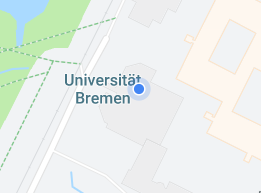
\includegraphics[width=\linewidth, height=4.5cm]{figures/map-app_examples/gm_positionsmarker}
        \captionof{figure}{Beispiel eines Positionsmarkers in Google Maps.}
        \label{fig:gm_positionsmarker}
        \vfill
    \end{minipage}
    \hfill
    \begin{minipage}[t]{.485\textwidth}
        \centering
        \vspace{0pt}
        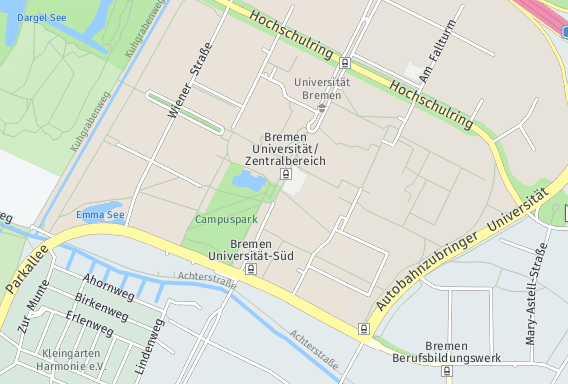
\includegraphics[width=\linewidth, height=4.5cm]{figures/map-app_examples/hwg_labels}
        \captionof{figure}{Beispiel von Labels in HERE WeGo.}
        \label{fig:hwg_labels}
    \end{minipage}
\end{figure}

\emph{Ortsmarkierungen} sind grafische Elemente, welche die Positionen von gewissen Gebäuden oder anderen interessanten Punkten (\emph{Points-of-Interest}, POI) auf Karten markieren.
Es gibt sowohl statische Ortsmarkierungen, die zusammen mit den Labels auf der Karte fest verankert sind, wie auch dynamische Ortsmarkierungen, die je nach Kontext des Nutzers ein- bzw. ausgeblendet werden.
Die dynamischen Ortsmarkierungen werden durch sogenannte \enquote{Stecknadeln} repräsentiert.
Diese sind mit Icons versehen, welche die Kategorie des POI anzeigen.
Beispiele finden sich in \autoref{fig:bm_gebaeudemarkierungen}.

Eine \emph{Klickmarkierung} kann in den Kartenanwendungen durch Klicken auf den Kartenbereich erzeugt werden.
Die Markierung wird grafisch als Stecknadel oder ein vergleichbares Symbol dargestellt (siehe \autoref{fig:gm_klickmarkierung}).
Über eine solche Markierung kann der Nutzer auf die Adresse und / oder die Koordinaten am angeklickten Ort zugreifen.
\begin{figure}[t]
    \centering
    \begin{minipage}[t]{.485\textwidth}
        \centering
        \vspace{0pt}
        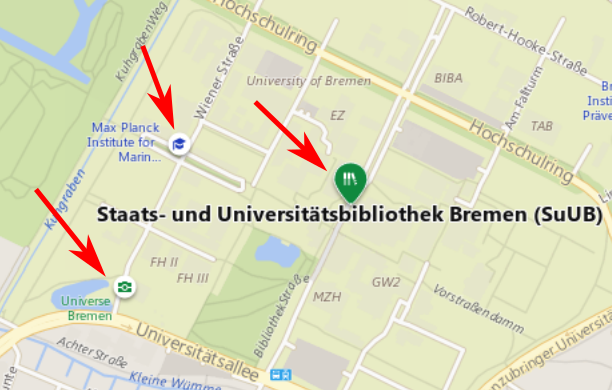
\includegraphics[width=\linewidth, height=4.5cm]{figures/map-app_examples/bm_gebaeudemarkierungen_arrows}
        \captionof{figure}{Beispiel von Ortsmarkierungen in Bing Maps (hervorgehoben durch \textcolor{red}{rote} Pfeile). %
        Ausgewählte Orte werden durch Stecknadeln stärker betont.}
        \label{fig:bm_gebaeudemarkierungen}
        \vfill
    \end{minipage}
    \hfill
    \begin{minipage}[t]{.485\textwidth}
        \centering
        \vspace{0pt}
        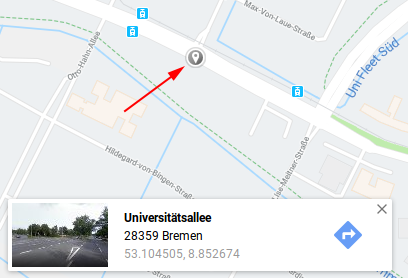
\includegraphics[width=\linewidth, height=4.5cm]{figures/map-app_examples/gm_klickmarkierung}
        \captionof{figure}{Beispiel der Klickmarkierung in Google Maps (hervorgehoben durch \textcolor{red}{roten} Pfeil). %
        Unterhalb der Markierung werden die Adresse und Koordinaten gezeigt.}
        \label{fig:gm_klickmarkierung}
    \end{minipage}
\end{figure}

Die \emph{spezifische Suche} ist eine Lokalisierungs-Interaktion, die durch ein Suchfeld ausgelöst wird.
Als \emph{spezifische} Suche (im Gegensatz zur \emph{offenen} Suche) wird in dieser Arbeit die Suche nach einer bekannten Adresse oder einem eindeutig benannten Ort verstanden (beispielsweise \enquote{Bremer Rathaus} oder \enquote{Bibliothekstraße 1}).
Wird eine solche Suche durchgeführt, platziert die Anwendung eine grafische Markierung auf dem Zielobjekt.
Den Nutzern bleibt somit eine manuelle Suche nach dem Zielort auf der Karte erspart.

Das letzte Lokalisierungselement ist die \emph{Attributsansicht}.
Über diese Ansicht werden Nutzern Informationen über einen Ort aufgelistet.
Die Informationen umfassen neben der Adresse und Anschrift unter anderem auch Kontaktdaten (Webseiten, Telefonnummern), Öffnungszeiten, Bilder, Bewertungen usw.
Speziell für Gebäude werden hier auch Ausstattungen gelistet.
\autoref{fig:gm_ausstattung} zeigt beispielsweise, wie in der Attributansicht von Google Maps die Ausstattung eines Hotels aufgelistet wird.
Die Anzeige solcher Informationen ermöglicht es, die Kartenanwendungen für andere Anwendungsfälle als die reine Navigation zu nutzen.
Dem obigen Beispiel folgend können Nutzer mit der Kartenanwendung ihre Unterkunft während einer Reise planen und werden dann zur Buchung auf die jeweilige Seite des Hotels weitergeleitet.
\begin{figure}[t]
	\centering
	\imagebox{
		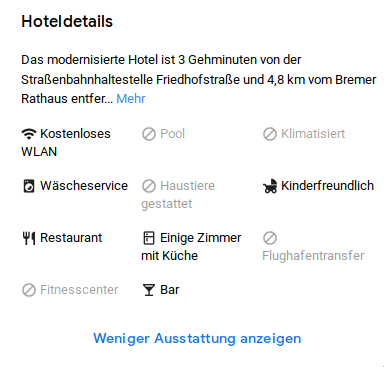
\includegraphics[height=7cm]{figures/map-app_examples/gm_ausstattung}
	}
	\caption{Beispiel für die Auflistung einer Gebäudeausstattung (eines Hotels in Bremen) in der Attributansicht von Google Maps.}
	\label{fig:gm_ausstattung}
\end{figure}

\subsection{Nähe-Elemente}
\label{ssec:prox-elements}
Nähe-Elemente sind Explorationselemente, die im Bezug zur Position des Nutzers stehen und eine Übersicht der näheren Umgebung des Nutzers ermöglichen.
Nutzer können diese Elemente verwenden, um sich ein Bild von der Umgebung zu machen.
Vor allem bei der offenen Suche nach unspezifischen Orten (z.B. \enquote{Restaurants in der Nähe}) kommen die Nähe-Elemente zum Einsatz, indem mehrere Alternativen als Zielorte angeboten werden.
Bei der Untersuchung der Beispielanwendungen ergaben sich acht Arten von Nähe-Elementen:

\emph{Positionsabhängige Ortsmarkierungen} sind, wie bereits in \autoref{ssec:loc-elements} beschrieben, grafische Elemente, die für den Nutzer relevante POI markieren.
Die Ortsmarkierungen werden zu einem Nähe-Element, wenn nur die Markierungen in der näheren Umgebung des Nutzers eingeblendet werden.
So können sich Nutzer auf nahegelegene Alternativen konzentrieren und die weiter entfernten Ziele ausblenden.
Erweitert wird dies in den untersuchen Anwendungen durch die \emph{zoomabhängigen Ortsmarkierungen}.
Hierbei werden Markierungen, die als weniger wichtig für den Nutzer betrachtet werden, erst bei einem hohen Zoom der Karte angezeigt.
Somit können vom Anbieter der Karte zum Beispiel beliebte, häufig frequentierte Ziele hervorgehoben werden, während wenig besuchte Ziele erst später eingeblendet werden.

\emph{Entfernungen} können als Nähe-Elemente außerhalb der reinen Navigation eingesetzt werden, um Nutzern eine konkrete Vorstellung der Umgebung zu erleichtern.
Nutzer können dadurch Reisezeiten abschätzen und bei mehreren Zielalternativen die mit dem kürzesten Reiseweg wählen.
Entfernungen werden zum Beispiel zusammen mit anderen Ortsinformationen angezeigt, oder Nutzer benutzen ein virtuelles Maßband zum Abmessen auf der digitalen Karte.

Die \emph{offene Suche} ist eine Nähe-Interaktion, die über ein Suchfeld ausgelöst wird.
Anders als die \emph{spezifische} Suche wird bei der offenen Suche nach Kategorien von Orten gesucht (z.B. \enquote{Restaurants}, \enquote{Parks}, \enquote{Zoo}).
Da bei einer solchen offenen Suche keine eindeutigen Ortsnamen verwendet werden, kommt es häufig zu mehreren Zielalternativen, die für die Nutzer zutreffen könnten.
In den untersuchten Anwendungen werden alle möglichen Alternativen durch Ortsmarkierungen hervorgehoben.
\autoref{fig:bm_open_search} zeigt eine offene Suche nach Hotels in Bremen.
\begin{figure}[h]
	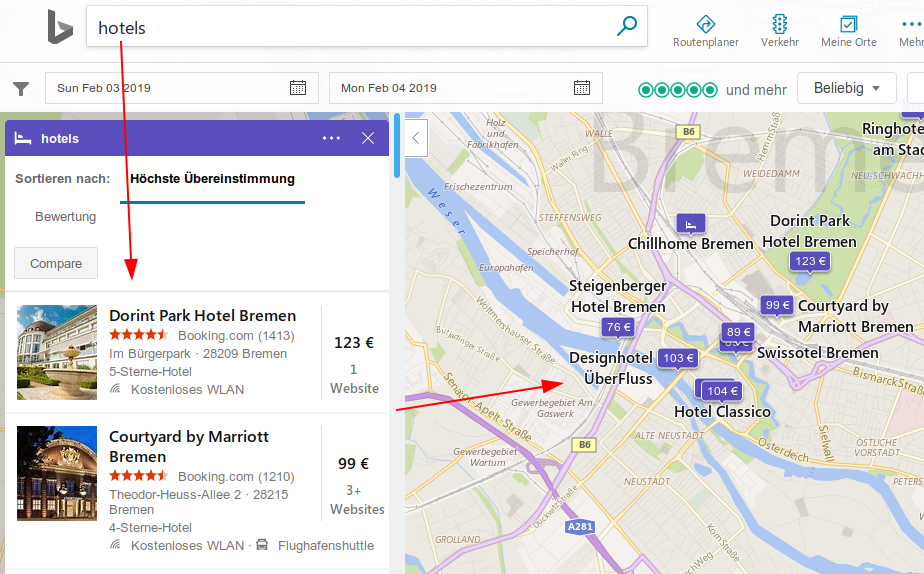
\includegraphics[width=\linewidth]{figures/map-app_examples/bm_open_search_2}
	\caption{Offene Suche nach Hotels in Bing Maps liefert mehrere Alternativen.}
	\label{fig:bm_open_search}
\end{figure}

Die \emph{Nahbereichssuche} ist eine Interaktion, mit der ein definierter Bereich der Karte unter Suchkriterien nach Orten durchsucht werden kann.
Damit ist sie eine lokal begrenzte offene Suche.
In den untersuchten Anwendungen lässt sich diese Funktion durch Öffnen des Kartenmenus mittels Rechtsklick aufrufen (siehe \autoref{fig:bm_nearby}).
Bei der Nahbereichssuche werden nur Ortsmarkierungen angezeigt, die sich in einem gewissen Radius um den Ort des Anklickens herum befinden.
Nutzer können hiermit Umgebungen erkunden, an denen sie sich selber nicht befinden.

Über die Elemente \emph{Filter und Sortierung} können die Suchkriterien weiter eingeschränkt werden.
Beispielsweise lassen sich Restaurants nach der gewünschten Küche filtern, oder Hotels nach Preisklasse (siehe \autoref{fig:bm_sorting}).
So müssen Nutzer nicht sämtliche verfügbare Alternativen per Hand durchgehen, um zu prüfen, ob die Alternativen ihren Vorstellungen entsprechen.
Die Filterung und Sortierung kann Nutzern somit durch das Ausblenden irrelevanter Orte Zeit beim Suchen von Zielen ersparen.

\begin{figure}[p]
    \centering
    \imagebox{
	    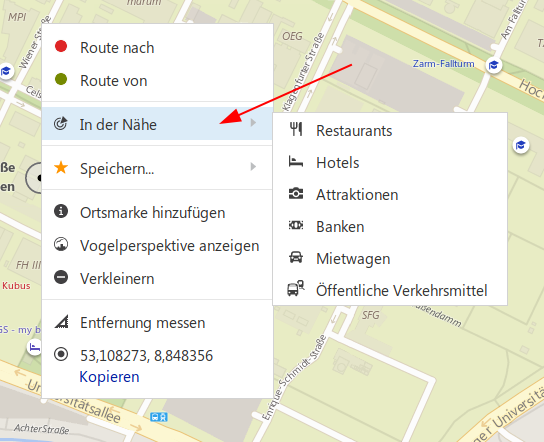
\includegraphics[width=0.485\linewidth]{figures/map-app_examples/bm_nearby}
	}
	\caption{Über das Rechtsklick-Menu in Bing Maps kann die Umgebung durchsucht werden.}
	\label{fig:bm_nearby}
\end{figure}
\begin{figure}[p]
	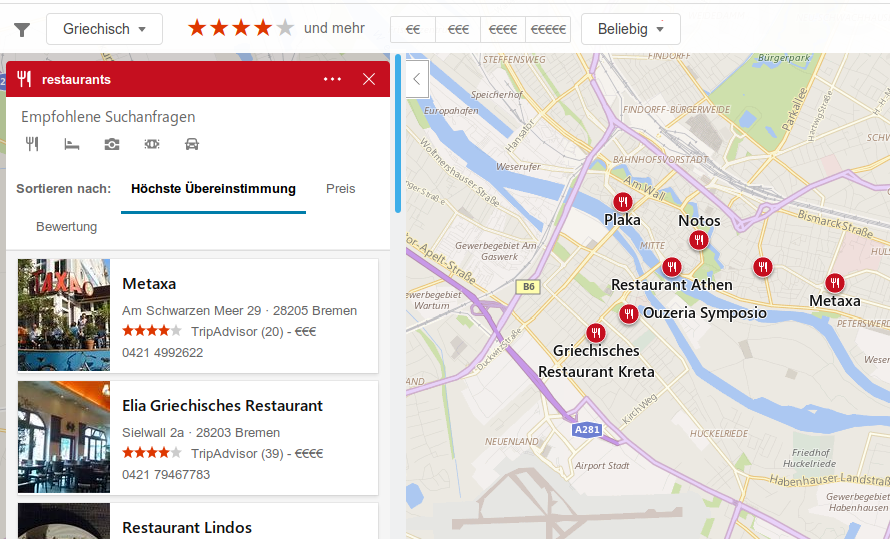
\includegraphics[width=\linewidth]{figures/map-app_examples/bm_filter_sorting}
	\caption{Anzeige und Sortierung von griechischen Restaurants mit einer 4-Sterne-Bewertung oder höher (in Bing Maps).}
	\label{fig:bm_sorting}
\end{figure}

Das Nähe-Element \emph{Ortsnachbarschaft} ist ein Element, welches in der Ansicht über die Ortsinformationen integriert sein kann.
Hierbei handelt es sich um eine List von weiteren Orten, die für den Nutzer relevant sein könnten und sich in der Nähe des aktuell betrachteten Orts befinden.
Auch die Information über nahegelegene Transportmöglichkeiten fällt unter diese Kategorie.

Schließlich finden sich \emph{Umgebungsbilder} in den Kartenanwendungen als Nähe-Element.
Sie zeigen Foto-Aufnahmen (gegebenenfalls als 360\textdegree-Aufnahme) der Umgebung.
Wie die Ortsmarkierungen sind die abgebildeten Orte auf einen gewissen Radius um einen Ausgangspunkt herum beschränkt, sodass für die Nutzer irrelevante Bilder nicht gezeigt werden.
Die Einbindung der Bilder in die Anwendungen wird unterschiedlich gehandhabt.
Zum Beispiel befindet sich in Google Maps eine Liste von Umgebungsfotos in Attributsansicht.
Wird die Liste angeklickt, öffnet sich eine Großansicht der Fotos (siehe \autoref{fig:gm_photos}).
Handelt es sich bei dem Bild um eine 360\textdegree-Aufnahme, kann mit der Maus die Ansicht verändert werden.
\begin{figure}[h]
	\centering
	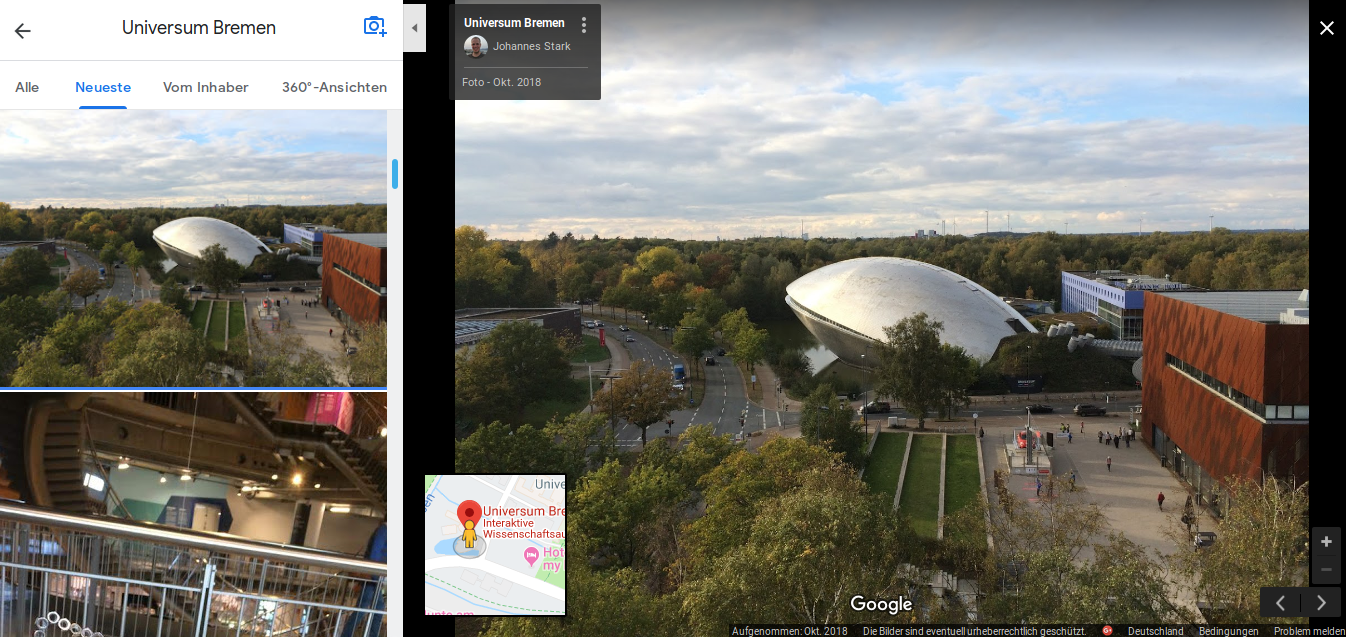
\includegraphics[width=\linewidth]{figures/map-app_examples/gm_photos_2}
	\caption{Umgebungsfotos zum Universum Bremen via Google Maps.}
	\label{fig:gm_photos}
\end{figure}

\subsection{Event-Elemente}
\label{ssec:event-elements}
Event-Elemente integrieren zeitliche Geschehnisse in die digitalen Karten.
Die Eventinformationen werden live aus diversen Datenquellen bezogen, wodurch die Karten in Echtzeit aktualisiert werden.
Bei der Untersuchung der Beispielanwendungen ergaben sich vier Arten von Event-Elementen:

Die \emph{Verkehrsinformationen} informieren Nutzer über die aktuelle Situation des Straßenverkehrs.
Verkehrsaufkommen, Baustellen, Staus und Umleitungen werden in Echtzeit in die Karten integriert und visualisiert.
Neben der aktuellen Verkehrssituation werden auch Durchschnittswerte für die Befahrung von Straßen angezeigt, sodass Nutzer bereits vorab den Verkehr in der Umgebung abschätzen können

Die \emph{Veranstaltungsinformationen} sind in die Ortsinformationen integriert.
Hier werden die Veranstaltungen der nächsten Tage präsentiert (z.B. Konzerte).
Unter Umständen werden auch die Ticketverfügbarkeit und -preise angezeigt.

\emph{Öffnungszeiten} informieren Nutzer über den Zugang zu Orten in der Umgebung, vor allem Gebäuden.
Dank der Integration der Öffnungszeiten müssen Nutzer nicht weitere Informationen abrufen, um zu schauen, ob das Ziel zur aktuellen Zeit erreicht werden kann.
Wie \autoref{fig:gm_opening_hours} zeigt sind beispielsweise die Öffnungszeiten in Google Maps in der Attributsansicht zu finden.

Zuletzt sind auch Informationen über das \emph{aktuelle Besucheraufkommen an Orten} als Event-Element verfügbar.
Nutzer können zum Beispiel einsehen, ob ein großer Andrang auf ein Geschäft besteht und so lange Wartezeiten beim Schlangestehen vermeiden (siehe \autoref{fig:gm_opening_hours}).
\begin{figure}[th]
	\centering
	\imagebox{
		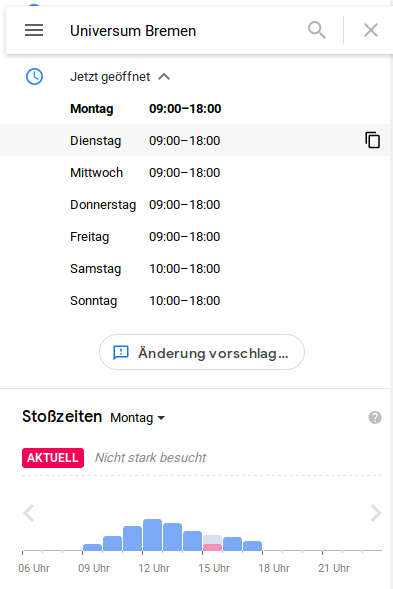
\includegraphics[width=0.4\linewidth]{figures/map-app_examples/gm_opening_hours}
	}
	\caption{Öffnungszeiten von Geschäften etc. werden in Google Maps in der Attributsansicht gezeigt.}
	\label{fig:gm_opening_hours}
\end{figure}

\section{Megamap in \emph{Tom Clancy's The Division}}
In \autoref{chap:einleitung} wurde bereits erwähnt, dass die grundlegende Idee für das Konzept der Megamap aus dem Spiel Tom Clancy's The Division stammt.
Anders als die zuvor beschriebenen Kartenanwendungen implementiert die Megamap in The Division eine dreidimensionale Karte, basierend auf einem virtuellen New York.
Die Karte wird in die Umgebung des Spielcharakters integriert, sodass dieser \enquote{in der Karte steht}.
Aus der Sicht des Spielcharakters handelt es sich also um eine AR-Karte.

Im Vergleich zu den vorigen Kartenanwendungen lassen sich sowohl Gemeinsamkeiten als auch Unterschiede bei der Umsetzung von Explorationselementen ermitteln.
Für diese Arbeit wird die Megamap aus The Division als vierte \enquote{Kartenanwendung} nach den gleichen Kriterien wie die anderen Anwendungen betrachtet.
Dieser Abschnitt geht auf die Explorationselemente in TCTDs Megamap ein.
Die Erkenntnisse über den Einsatz von Explorationselementen in TCTDs Megamap fließen in die Gestaltung des Megamap-Konzepts dieser Arbeit ein.
Eine Übersicht der gefundenen Elemente findet sich (zusammen mit denen der anderen Anwendungen) in \autoref{tab:exploration_elements_summary}.

Das Aufrufen der Megamap in TCTD geschieht in zwei Schritten (siehe \autoref{fig:tctd_overview}):
\begin{enumerate}
    \item Ein kleiner Ausschnitt der Megamap wird um den Spielcharakter herum in die virtuelle Umgebung integriert.
    Falls sich dort bereits Objekte befinden, bleiben diese weiterhin sichtbar.
    Die Megamap ist an den Überschneidungspunkten komplett transparent.
    \item Sobald der Zoom oder die Verschiebung der Megamap durch den Spieler geändert wird, wird ein größerer Ausschnitt der Megamap gezeigt.
    Die virtuelle Umgebung wird ausgeblendet und wird nur noch durch die Megamap skizziert.
\end{enumerate}
\begin{figure}[hbt]
    \centering
    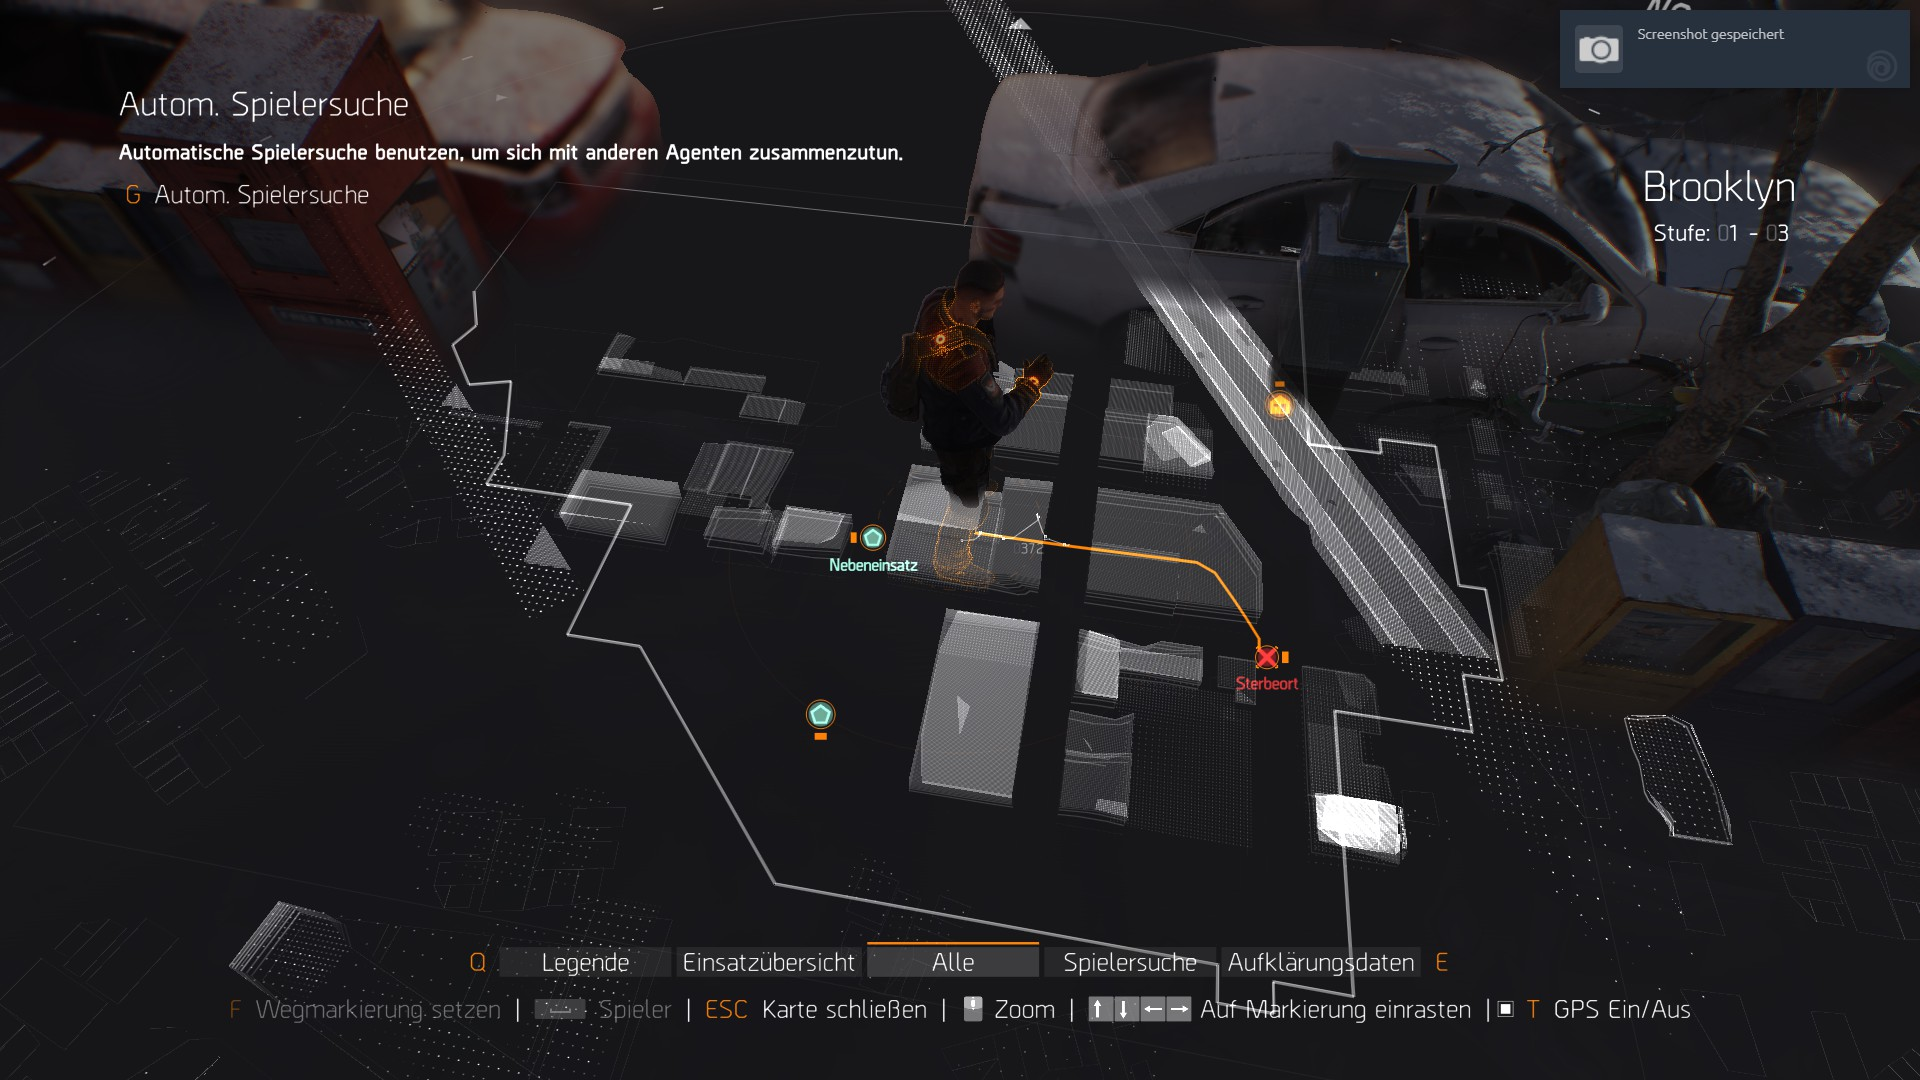
\includegraphics[width=\linewidth]{figures/concept/the_division_overlap}

    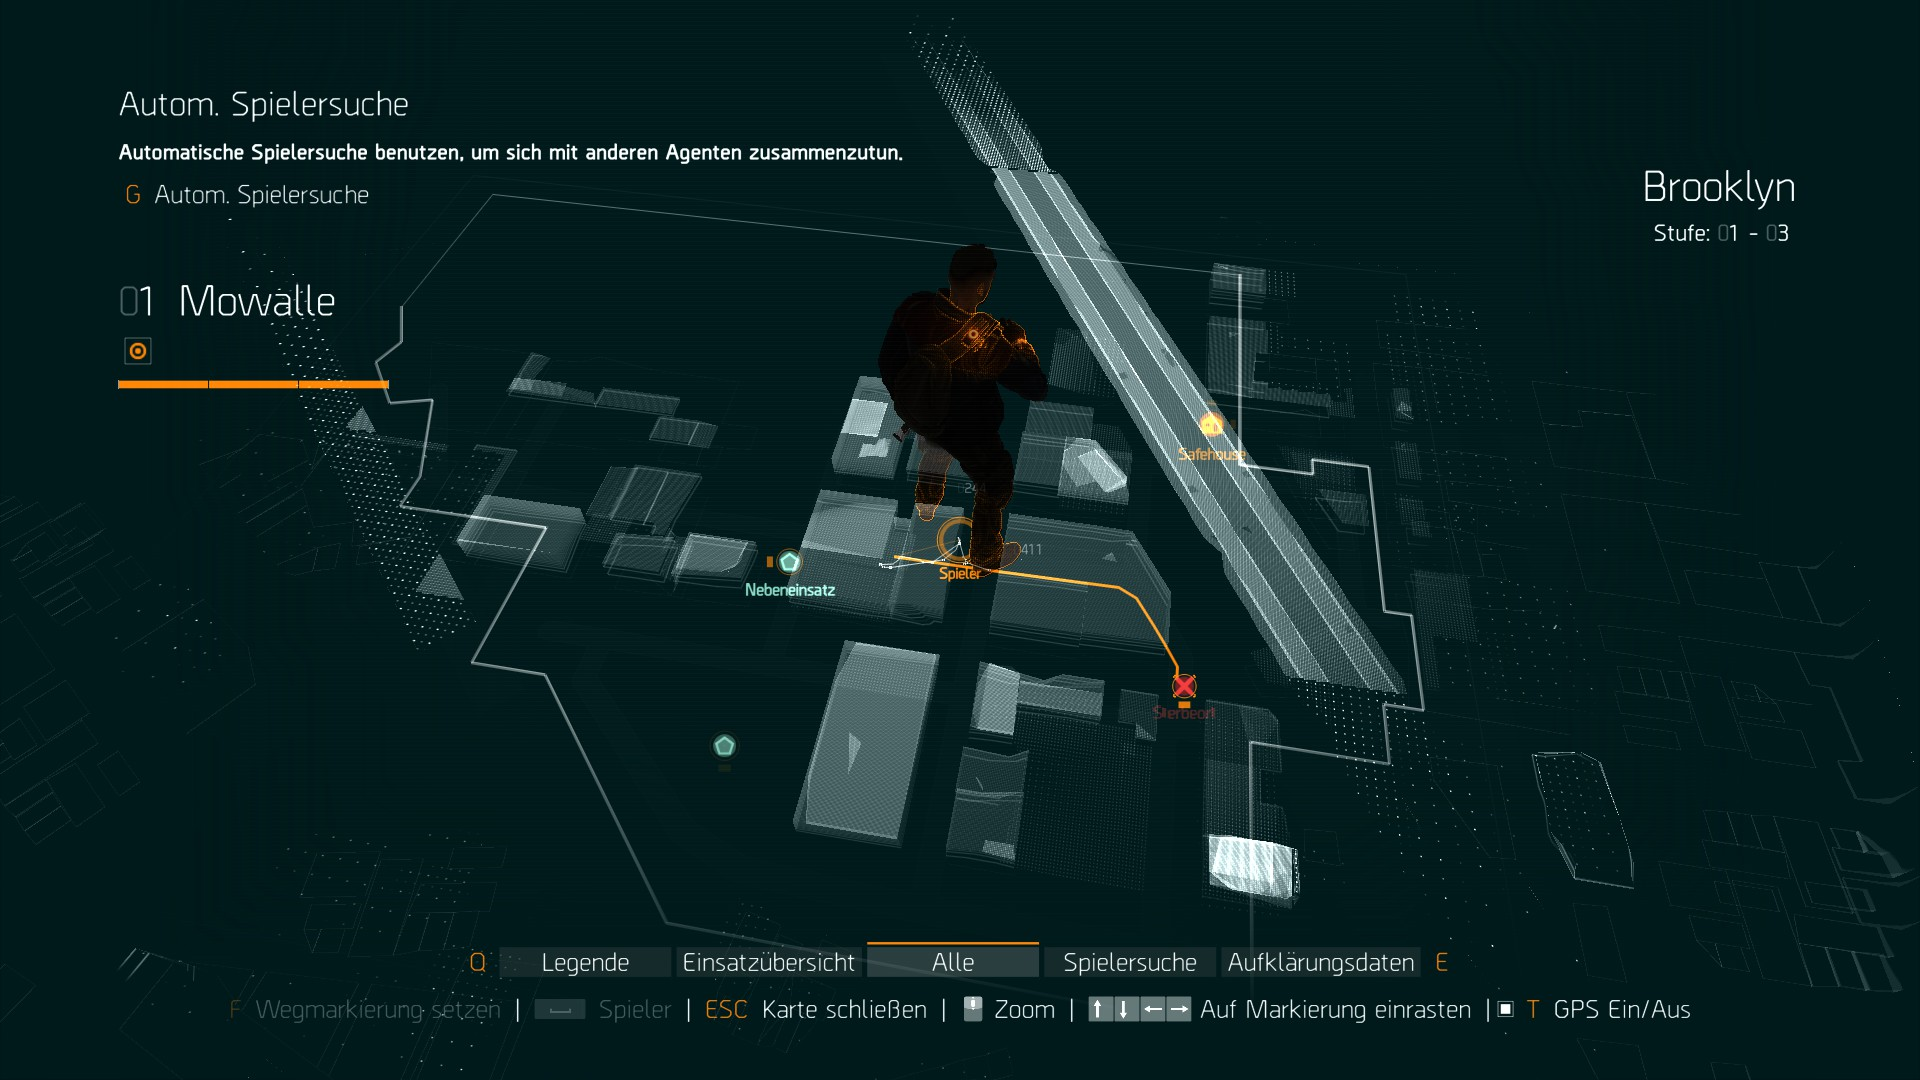
\includegraphics[width=\linewidth]{figures/concept/the_division_5}
    
    \caption{Übersicht der Magamap in TCTD.}
    \label{fig:tctd_overview}
\end{figure}

Die Megamap nutzt einige der Lokalisierungselemente, die auch in der anderen Anwendungen zu finden sind.
Ein Positionsmarker zeigt die aktuelle Position des Spielecharakters in der Welt an, wenn die Kamera nahe an die Karte herangezoomt wird (ansonsten wird weiterhin der Spielecharakter dargestellt).
Straßen, Parks, Stadtteile etc. werden durch Text-Labels benannt.
Wichtige Punkte auf der Karte (wie zum Beispiel andere Spieler, Missionen, Gebäude oder Items) werden durch unterscheidbare Icons und ergänzenden Text markiert.
So können Spieler Orte auf der Karte schneller entdecken.
Mit dem Controller können Spieler einen Cursor über die Megamap bewegen, der dabei x- und y-Koordinaten der Karte anzeigt.
Drücken die Spieler einen entsprechenden Knopf, können sie eine Klickmarkierung auf der Karte platzieren, welche automatisch eine Route vom Spielcharakter zum angeklickten Ort berechnet.
\autoref{fig:tctd_clickmarker} zeigt einen Screenshot von der Klickmarkierung.
\begin{figure}[h]
    \centering
    \imagebox{
        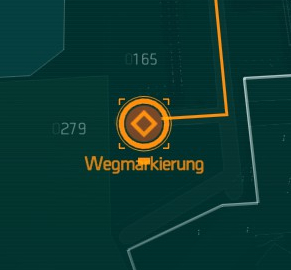
\includegraphics[width=0.3\linewidth]{figures/concept/the_division_clickmarker_x}
    }
    \caption{Klickmarkierung in TCTDs Megamap mit x-/y-Koordinaten.}
    \label{fig:tctd_clickmarker}
\end{figure}

Falls sich stattdessen eine Markierung am angeklickten Ort befindet, werden diverse Eigenschaften des Orts auf einem HUD der Karte angezeigt.
Beispielsweise werden bei einer Mission das notwendige Charakterlevel, die Missionsbeschreibung sowie die Belohnungen für einen Missionsabschluss aufgelistet.
Zudem werden die Entfernungen der Orte zum Spielcharakter angezeigt.
Dies entspricht der Attributsliste für Orte aus den anderen Anwendungen.
\autoref{fig:tctd_attributes} zeigt, wie die Daten zu einem Ort im HUD angezeigt werden, wenn Spieler einen Ortsmarker anklicken.
\begin{figure}[h]
    \centering
    \imagebox{
        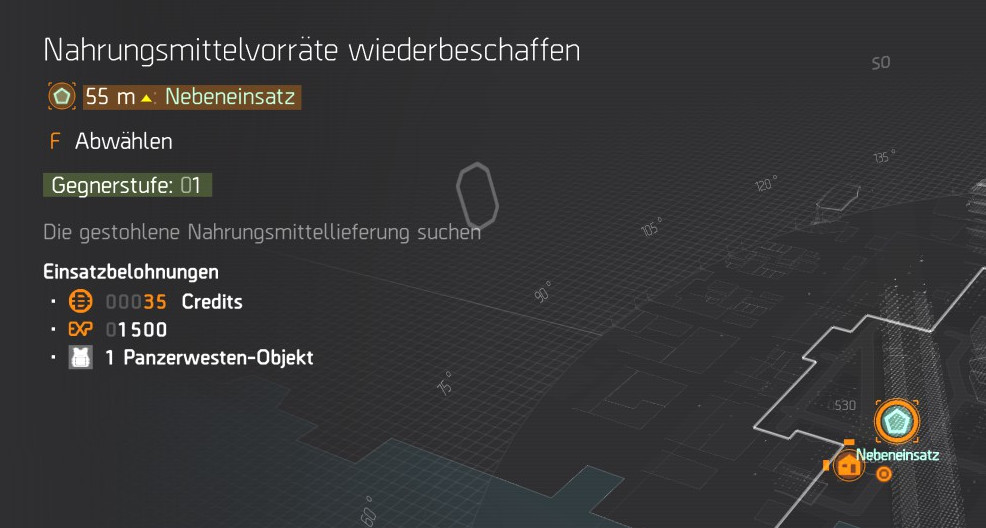
\includegraphics[width=\linewidth]{figures/concept/the_division_attributes_x}
    }
    \caption{Durch Anklicken eines Ortsmarkers werden die jeweiligen Daten zum Ort im HUD angezeigt.}
    \label{fig:tctd_attributes}
\end{figure}

Nähe-Elemente, wie es sie in den anderen Anwendungen gibt, sind in TCTD weniger zu finden.
Neben den positions- und zoomabhängigen Ortsmarkierungen sowie den bereits erwähnten Entfernungsangaben bietet die Megamap in TCTD nur eine limitierte Funktionalität zum Filtern der Ortsmarkierungen.
Sortierungen der Markierungen, Umgebungsbilder sowie eine offene Suche sind in der Megamap nicht vorhanden.

Ebenso sind keine Eventelemente vorhanden, wie es sie in den anderen Anwendungen gibt.
Stattdessen werden die Positionen von anderen Mitspielern, Gegnern und Missionszielen in Echtzeit auf der Megamap gezeigt.

Da es sich bei der Megamap aus der Sicht des Spielcharakters um eine AR-Karte handelt, setzt sie einige Funktionen um, die mit den anderen Anwendungen nicht möglich sind.
Durch ihre Platzierung im 3D-Raum kann sie die Umrisse der Gebäude des virtuellen New Yorks auch in der Höhe darstellen.
Um die Megamap herum wird ein augmentierter Kompass-Ring eingeblendet, der den Spielern die Himmelsrichtungen anzeigt.
Außerdem ist die Megamap mit einer augmentierten \enquote{GPS}-Routenführung für den Spielcharakter integriert.
Dabei zieht sich eine Line durch die virtuelle Umgebung, welche den Spielern den Weg zu ausgewählten Zielen zeigt.
Einen Beispielscreenshot vom AR-GPS in TCTD findet sich in \autoref{fig:tctd_at-gps}.
\begin{figure}[h]
    \begin{minipage}{0.5\linewidth}
        \centering
        \vspace{0pt}
        \raisebox{-0.5\height}{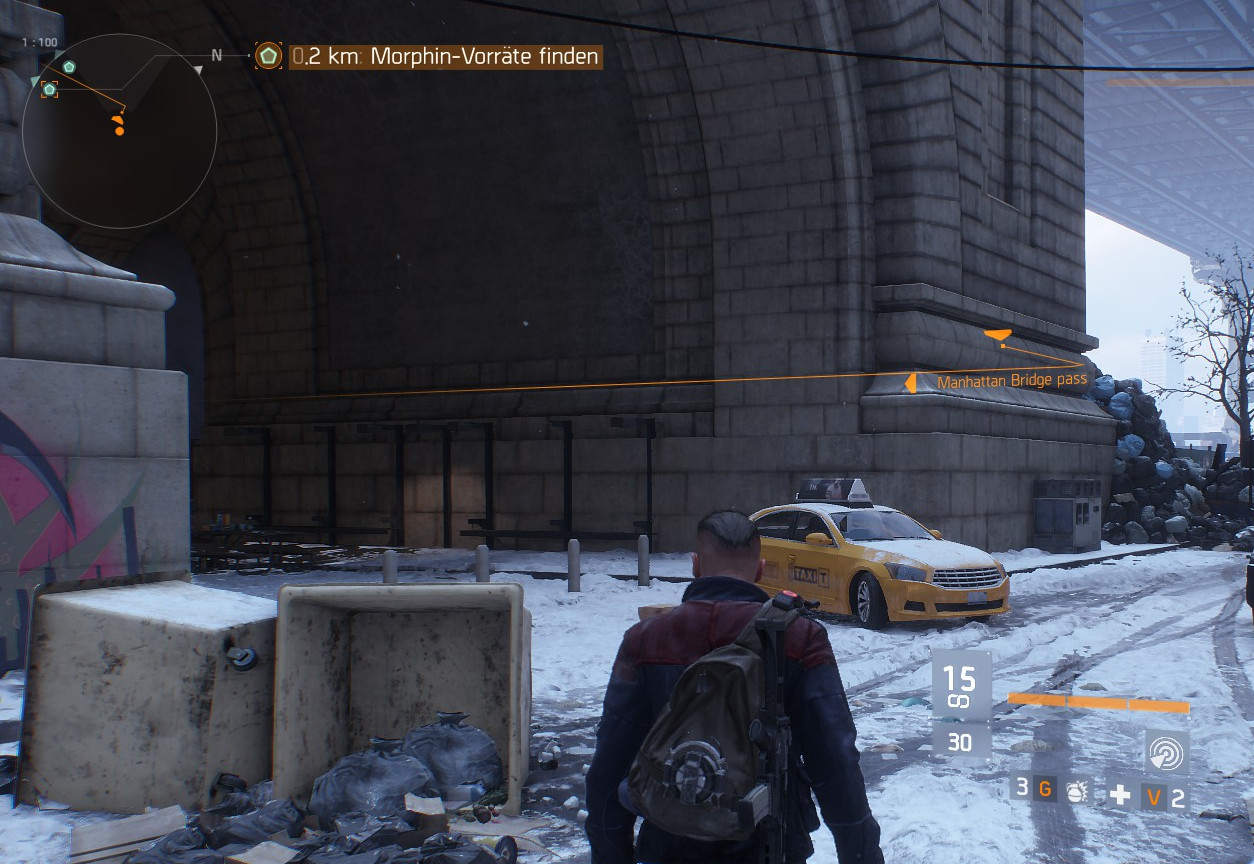
\includegraphics[width=\linewidth]{figures/concept/the_division_gps_x}}
    \end{minipage}%
    \hfill
    \begin{minipage}{0.48\linewidth}
        \centering
        \vspace{0pt}
        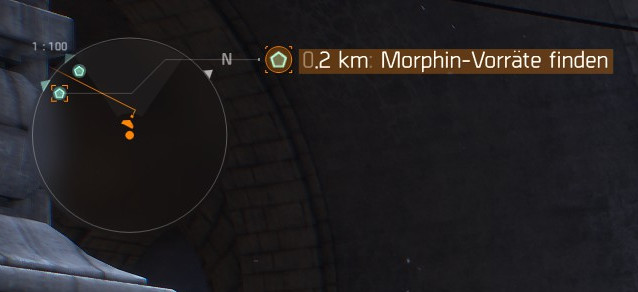
\includegraphics[width=\linewidth]{figures/concept/the_division_minimap}
        
        \vspace{1em}
        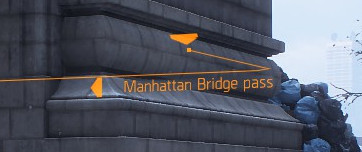
\includegraphics[width=\linewidth]{figures/concept/the_division_arrow}
    \end{minipage}
    \caption{Wegpunkt in Megamap kontrolliert das augmentierte GPS. %
    Oben~Rechts: Minikarte. %
    Unten~Rechts: Das GPS führt in Richtung \enquote{Manhattan Bridge pass}.}
    \label{fig:tctd_ar-gps}
\end{figure}

Viele Aspekte der Megamap in TCTD sind für die Umsetzung einer AR-Kartenanwendung in der realen Welt interessant.
Für die Realisierung einer solchen Anwendung ergeben sich jedoch Probleme, die gelöst werden müssen.
Zum Beispiel ist im Spiel ein 3D-Modell der Umgebung implizit gegeben, da die Umgebung selbst aus 3D-Modellen aufgebaut ist.
In der realen Welt sind solche Modelle der Umgebung unter Umständen nicht verfügbar.
Damit eine Megamap dargestellt werden kann müssen Daten von der Umgebung bekannt sein.
Ein weiteres Problem ist die Integration der Karte in die Umgebung.
Da im Spiel alle Umgebungsobjekte wie die Karte virtuell sind, können Überlappungen der Karte mit den Objekten durch visuelle Effekte wie in TCTD umgangen werden.
In der realen Welt müssen die Objekte der MR-Anwendung bekannt sein, um Überlappungen korrekt berechnen zu können.
Außerdem ist die Megamap in TCTD nicht für den Spiel\emph{charakter}, sondern für den \emph{Spieler} selbst gedacht.
Das heißt, der Spieler betrachtet sowohl die virtuelle Umgebung als auch die Karte aus einer Dritte-Person-Perspektive.
In der realen Welt nehmen Nutzer jedoch die Erste-Person-Perspektive ein, wodurch die Perspektive auf die Megamap eine andere wäre, als die im Spiel.
Es ist also nicht klar, ob sich das Konzept der Megamap auf die Anwendung in der Ersten-Person-Perspektive in der echten Welt übertragen lässt.

Auf diese Probleme wird im weiteren Verlauf der Arbeit durch die Aufstellung eines Megamap-Konzepts, dessen prototypischer Implementierung sowie einer Nutzerstudie des Prototypen eingegangen.

\section{Das Megamap-Konzept}
Basierend auf den Erkenntnissen der vorigen Abschnitte kann ein Konzept für eine umgebungsintegrierte Megamap entwickelt werden, deren Zielplattform Mixed-Reality-HMDs sind.

\subsection{Nutzungsszenario}
Die Megamap als eine dreidimensionale Karte für MR-HMDs konzipiert.
Vor dem Hintergrund der Umgebung des Nutzers zeigt sie ein dreidimensionales Innenmodell des Gebäudes, in dem sich der Nutzer zur Zeit befindet.
Die Karte wird durch das HMD in die Umgebung des Nutzers integriert.
Vor allem bleibt ihre Rotation in der Umgebung verankert, wenn der Nutzer sich bewegt.
Somit erscheint es, als würde die 3D-Karte tatsächlich in der Umgebung stehen.
Für mehrstöckige Gebäude wird nur das aktuelle Stockwerk angezeigt, wobei Nutzer die Möglichkeit zum Wechsel der Stockwerke haben.
Über Interaktionselemente ist es möglich, Informationen zu Räumen und Objekten auf der Karte abzurufen.
Die Konzeptzeichnung in \autoref{fig:concept_overview} verdeutlicht das Prinzip.

Die Megamap soll Nutzern helfen, sich in unbekannten Gebäuden zu orientieren, diese zu erkunden und nach Orten in den Gebäuden zu suchen.
Ein Beispiel ist die augmentierte Exploration der Gebäude der Universität Bremen.
Neue Studierende oder Gäste der Universität könnten durch die Megamap bei der Suche nach Büros von Mitarbeitern, öffentlichen Druckern, Essensmöglichkeiten, Toiletten etc. unterstützt werden.
Da die meisten der Universitätsgebäude mehrstöckig sind, wäre der Einsatz einer dreidimensionalen Karte zur Exploration der Gebäude interessant.
Auch der Einsatz in Einkaufszentren oder Flughäfen ist denkbar.
\begin{figure}[bht]
	\centering
	\imagebox{
		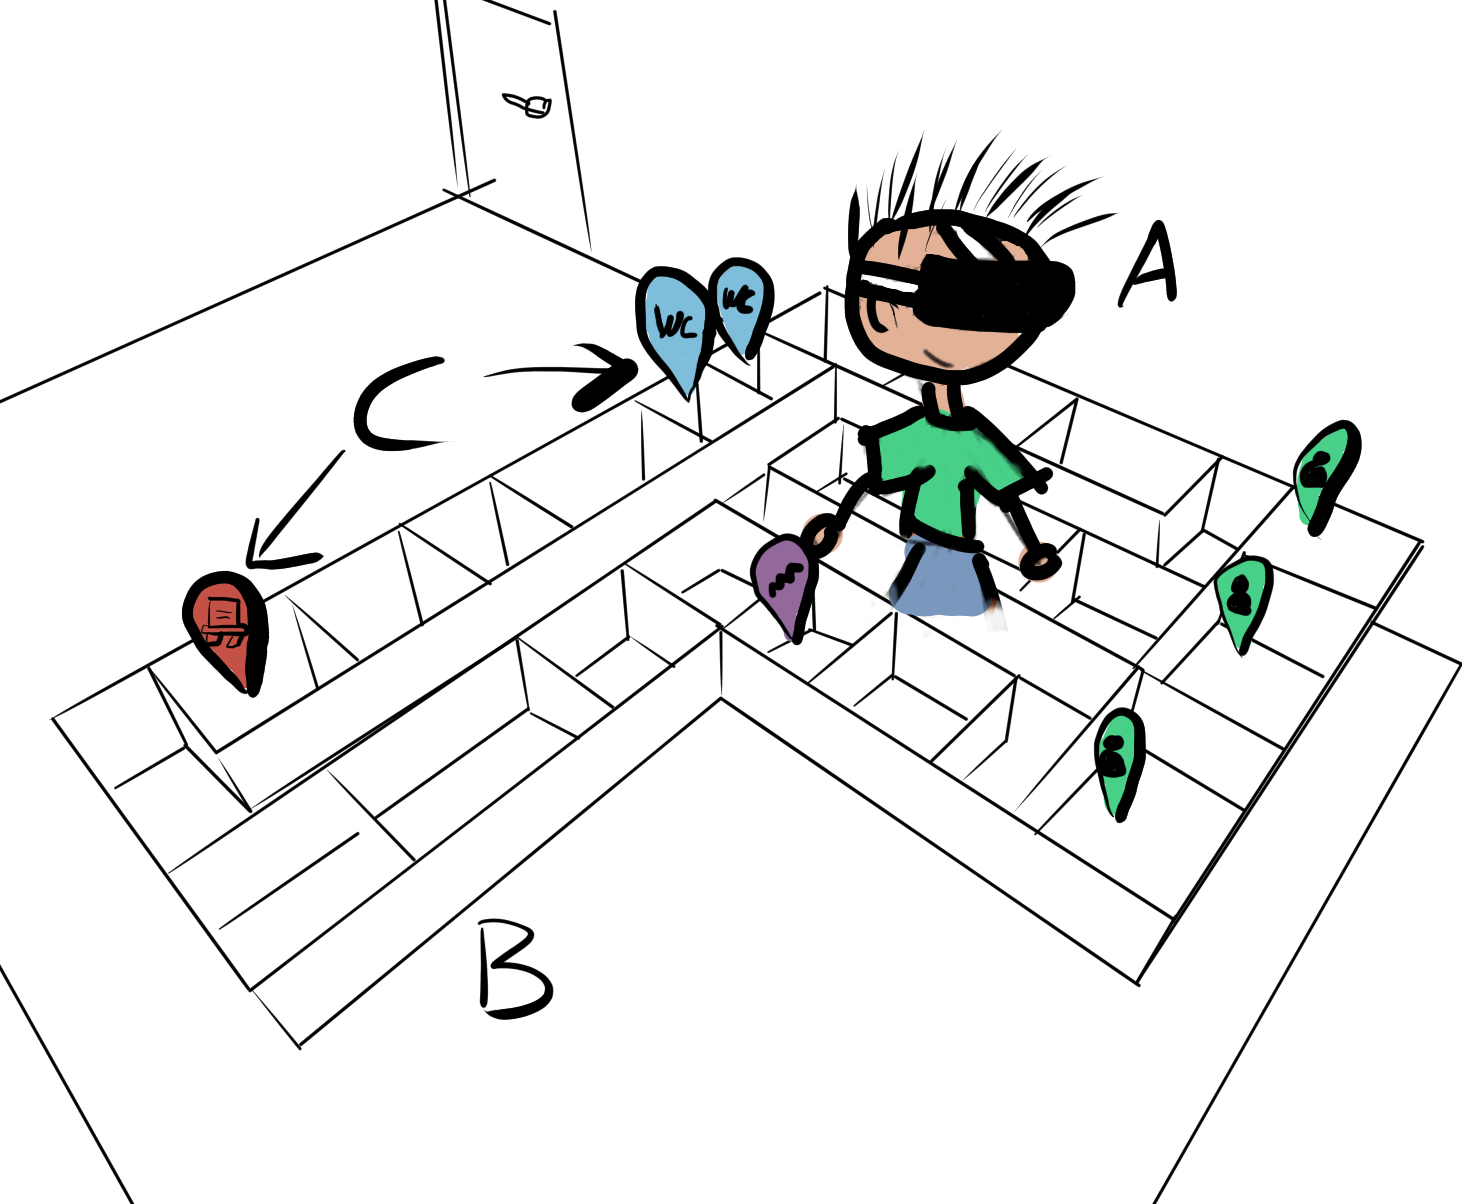
\includegraphics[width=0.75\linewidth]{figures/concept/overview}
	}
	\caption{Konzeptzeichnung einer Megamap. %
		A:~Nutzer trägt ein HMD. %
		B:~Indoor-Megamap wird in Umgebung des Nutzers angezeigt. %
		C:~Stecknadel-Icons markieren Räume mit Kategorien.}
	\label{fig:concept_overview}
\end{figure}

\subsection{Interaktion durch Explorationselemente}
\todo{Kon\-zept\-zeich\-nun\-gen überarbeiten.}
Nutzern von MR-HMDs wie der HoloLens oder der Magic~Leap stehen drei Eingabemethoden zur Verfügung: Controller, Gesten- und Sprachsteuerung.
Da die Megamap in dieser Arbeit als Prototyp in VR implementiert wird, konzentriert sich das Konzept auf die Controller-Methode.

Damit das 3D-Gebäudemodell überhaupt als Karte fungieren kann, müssen Nutzer mit dem Modell interagieren können.
Speziell muss die Karte Explorationselemente anbieten, mit denen Nutzer die Umgebung erkunden können.
Mögliche Explorationselemente sind in \autoref{sec:exploration_elements} beschrieben.
Für das entwickelte Konzept sowie den Prototypen wurde eine kleinere Auswahl der Elemente betrachtet.
Ein Ziel für zukünftige Arbeiten kann daher sein, dass die Megamap die gleiche Zahl an Explorationselementen unterstützt wie herkömmliche 2D-Kartenanwendungen.

Für die Indoor-Megamap werden die Ortsmarkierungen als \emph{Raum}markierungen umfunktioniert, da bei der Anwendung nur ein Gebäude zur Zeit im Fokus steht.
Die Raummarkierungen werden als dreidimensionale Stecknadeln über Räumen mit besonderen Funktionen dargestellt.
So können interessante Orte im Gebäude hervorgehoben werden.
Durch Icons auf den Stecknadeln kann die Kategorie des Raums hervorgehoben werden (beispielsweise Büro, Toilette etc.).
Ebenso können mit den Stecknadeln wichtige Objekte im Gebäude markiert werden (Drucker, Treppen und Aufzüge, Erste-Hilfe-Kästen etc.).
Über Filterelemente neben der Karte ließen sich dann Stecknadeln einer Art herausfiltern.
Die Konzeptzeichnung in \autoref{fig:concept_indoor_view} zeigt die Indoor-Megamap der Ebene 5 des MZH an der Universität Bremen.
Über eine virtuelle Filterbox werden nur Stecknadeln für öffentliche Toiletten gezeigt.
Stecknadeln werden auch über Stockwerke hinweg angedeutet, indem sie vertikal versetzt und transparent gemacht werden.
So können Nutzer auch Orte und Objekte finden, die auf dem aktuellen Stockwerk nicht vorhanden sind.
\vfill
\begin{figure}[h]
	\centering
	\imagebox{
		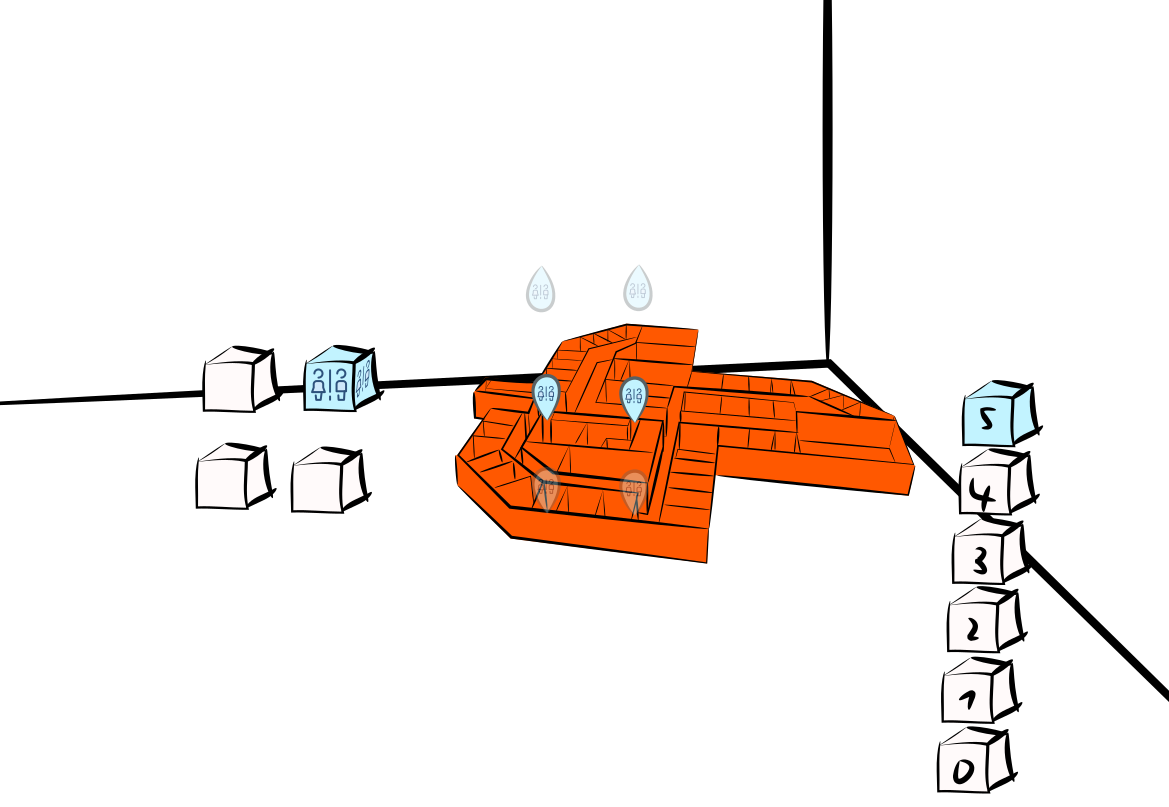
\includegraphics[trim={4cm, 0, 3cm, 5cm}, clip, width=0.7\linewidth]{figures/concept/3d_condition}
	}
	\caption{Konzeptzeichnung Megamap für Stockwerkwechsel, Filter und Suche.}
	\label{fig:concept_indoor_view}
\end{figure}

Um mehr Informationen zu einem Ort oder Objekt zu erhalten, können Nutzer die Stecknadel entweder mit dem im Raum getrackten Controller berühren, oder sie mit einem virtuellen Laserpointer anvisieren.
Letztere Variante hat den Vorteil, dass sich Nutzer nicht zu weiter entfernten Stecknadeln hinbewegen müssen.
An der Position des Pins öffnet sich ein Fenster mit Informationen zum Ort bzw. Objekt, was die Aufgabe der Attributsliste aus \autoref{sec:exploration_elements} übernimmt.
Ein Beispiel für ein solches Informationsfenster ist in \autoref{fig:concept_pin_info} skizziert.
Wie die Karte und die Stecknadeln ist auch das Informationsfenster in der Umgebung verankert.
Anstatt es direkt auf dem Display des Nutzers anzuzeigen befindet sich das Fenster an der Position der Stecknadel und wird so rotiert, dass der Nutzer immer auf die Vorderseite schaut.
Seine relative Position zur Umgebung bleibt gleich.
Eine Integration von 2D-Elementen als 3D-Objekt in die Umgebung (anstatt fester Anzeige auf dem Display) verhindert Unwohlsein bei Nutzern sowie eine Verdeckung der Umgebung und anderer virtueller Inhalte \parencite[23]{Schroeder2017}.

Damit Nutzer das aktuell gezeigte Stockwerk wechseln können, ohne sich physisch dorthin zu bewegen, werden weitere virtuelle Schaltflächen angeboten (siehe \autoref{fig:concept_indoor_view}).
Mit diesen kann auf die gleiche Weise wie mit den Stecknadeln oder den Filterelementen über den Controller interagiert werden.

Damit Nutzer ihre Position auf der Karte schnell erkennen können wird der Positionsmarker als Lokalisierungselement für die Megamap übernommen.
Für die Anwendung auf einer 3D-Karte wird der Marker von einem zweidimensionalen Kreis zu einem Zylinder erweitert.
Zusätzlich zeigt ein Kreissegment die aktuelle Blickrichtung sowie den Blickwinkel des Nutzers an.
Somit können Nutzer nicht nur ihre Position, sondern auch ihre Orientierung innerhalb der Umgebung vom Positionsmarker ablesen.

\begin{figure}[bth]
	\centering
	\imagebox{
		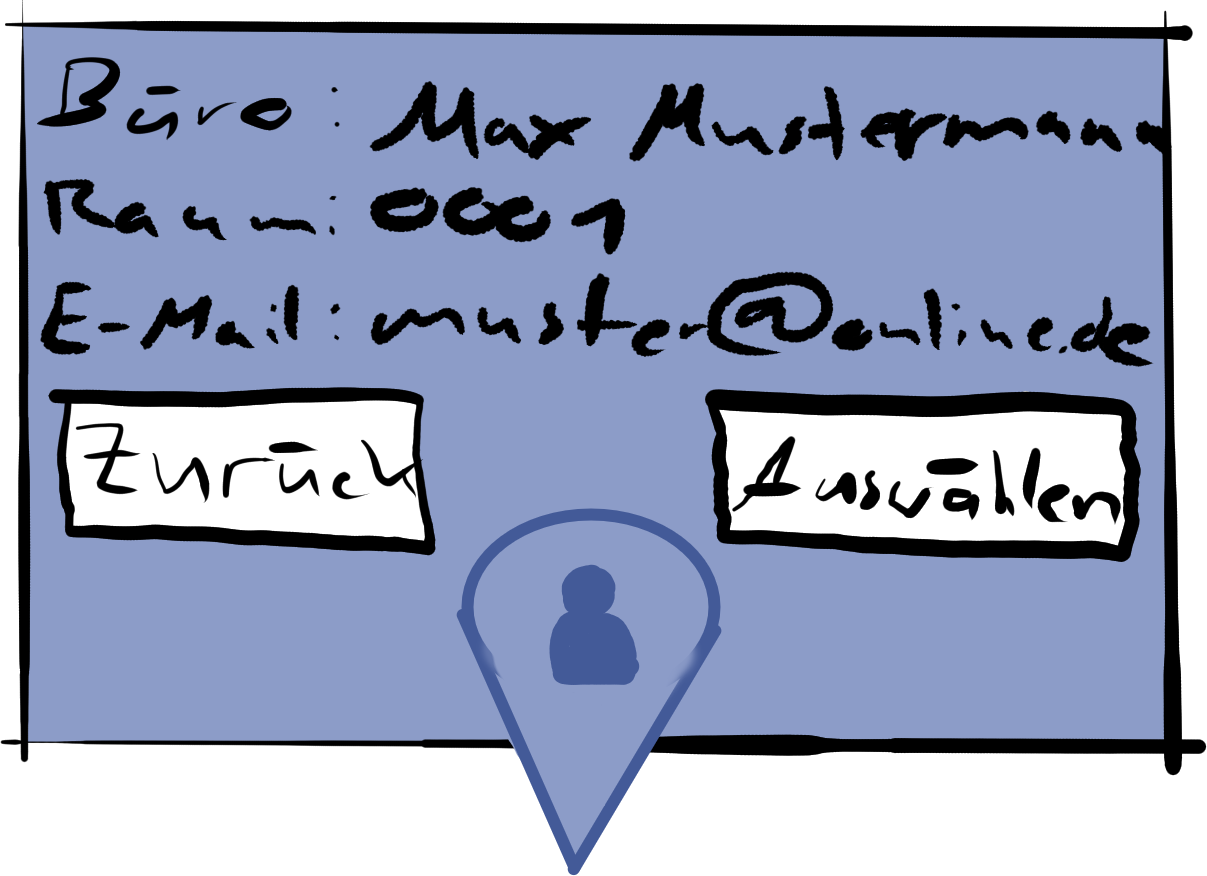
\includegraphics[width=0.72\linewidth]{figures/concept/concept_location_info}
	}
	\caption{Konzeptzeichnung der Stecknadel-Informationen.}
	\label{fig:concept_pin_info}
\end{figure}

\subsection{Platzierung der Megamap im Raum}
Um die Megamap wie ein \enquote{reales} Objekt im Raum zu platzieren wird die 3D-Rekonstruktion des HMDs eingesetzt.
Durch die Rekonstruktion liefert das HMD 3D-Meshes des Bodens, der Wände und vereinfachte Meshes von Objekten der Umgebung.
Die Megamap kann auf dem Boden-Mesh platziert werden, sodass sie in der realen Umgebung ebenfalls auf dem Boden steht.
Durch einen Abstand zum Boden-Mesh wirkt es, als würde die Megamap im Raum schweben.

Analog zur Karte aus TCTD soll die Megamap so um den Nutzer herum platziert werden, dass die Position des Nutzers auf der Karte mit seiner aktuellen Position übereinstimmt.
Das bedeutet, dass zu Beginn (beim Aufrufen der Karte) der Nutzer auf seiner eigenen Markierung steht.
Dies soll Nutzern eine schnellere Orientierung ermöglichen, da sie ihre Position auf der Karte nicht erst wiederfinden müssen.
Damit die Position der Nutzer bestimmt werden kann ist ein System zur Indoor-Lokalisierung erforderlich.
Mehrere Ansätze werden in der Literatur diskutiert, darunter \wifi-Fingerprinting \parencites{Lautenschlaeger2012}{Alnabhan2014}, Magnetfeld-Fingerprinting \parencites{Hashish2017}{Ang2018} oder Bild-basierte Verfahren \parencites{Kalkusch2002}{Moeller2014}{Silva2015}.
Weiterhin könnten die vom HMD gelieferten 3D-Meshes mit vorgefertigten Raummodellen abgeglichen werden, um den aktuellen Raum sowie die aktuelle Position des Nutzers zu bestimmen.

Ein Problem, was bei der Platzierung der virtuellen Karte in die reale Umgebung auftritt, ist die Verdeckung realer Objekte.
Durch eine Verdeckung, bei der Teile des realen Objekts noch sichtbar sind, entsteht eine Störung des Tiefeneindrucks des Nutzers, wodurch der Effekt einer integrierten Karte verloren geht.
TCTD löst das Problem der Verdeckung von Umgebungsobjekten, indem die Karte an den Schnittpunkten mit den Objekten immer weiter ausgeblendet wird, bis schließlich nur noch die Objekte zu sehen sind.
Die Karte wird effektiv an den Objekten \enquote{ausgeschnitten}.
Mit den erwähnten MR-HMDs ist ein solcher Effekt ebenfalls möglich.
Durch die 3D-Rekonstruktion ergeben sich grobe Meshes der Umgebungsobjekte und Wände.
Die virtuelle Megamap kann an den Stellen dieser Meshes transparent gerendert werden, wodurch der Effekt aus TCTD nachgestellt wird.

\subsection{Beschaffung von Gebäudedaten und Generierung der Karten}
Für die Darstellung als Megamap ist ein 3D-Modell des Gebäudes erforderlich.
Eine automatisierte Generierung des Modells basierend auf Gebäudedaten ist wünschenswert, damit das Modell nicht per Hand erstellt werden muss und immer die aktuellsten Daten des Gebäudes nutzt.
Ein möglicher Ansatz ist, die Grundrisse des jeweiligen Gebäudes zu georeferenzieren und in einer entsprechenden Datenbank wie z.B. OpenStreetMap zu veröffentlichen.
Die Megamap-Anwendung kann auf die georeferenzierten Grundriss-Daten über die Programmierschnittstelle (\emph{Application Programming Interface} (API)) zugreifen und daraus 3D-Modelle generieren.
Die Wände des Gebäudes können z.B. als Polygon-Features mit dem OSM-Tag \lstinline{height} angelegt werden, die Türen würden durch Rechtecke mit dem Tag \lstinline{min_height} repräsentiert.
Normalerweise werden in OSM mit diesen Tags Gebäude als Ganzes definiert \parencite{OpenStreetMapFoundation2018b}.
Dennoch lassen sich die Tags für die Definition eines Indoor-Layouts umfunktionieren.

Ergänzend hierzu unterstützt OSM das \emph{Simple Indoor Tagging Schema}.
\autoref{fig:osm_simple-indoor-tagging} zeigt, wie das Schema auf ein Gebäudelayout angewendet werden kann.
Da dieses Schema zum regulären Tagging in OSM kompatibel ist, können Indoor- und Outdoor-Daten in der selben Datenbank verwaltet werden \parencite{OpenStreetMapFoundation2018c}.
\begin{figure}[t]
    \centering
    \imagebox {
        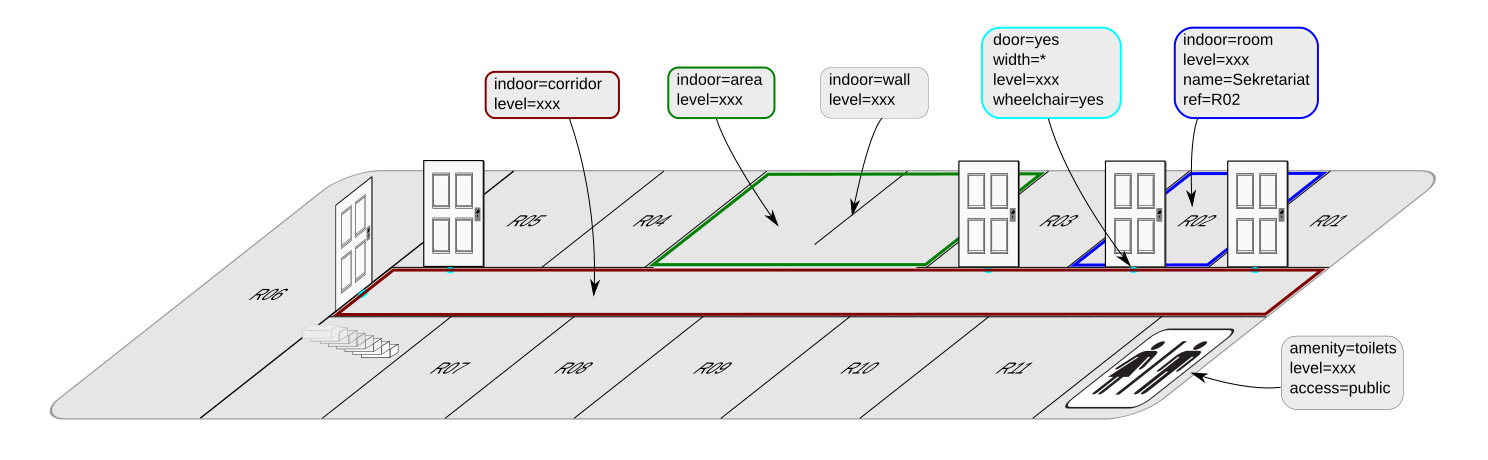
\includegraphics[trim={17cm, 0, 0, 0}, clip, width=\linewidth]{figures/concept/osm_Indoor2_0_elements}
    }
    \caption{Beispiel des Simple Indoor Tagging Schemas in OpenStreetMap. %
    \quelle{\cite{OpenStreetMapFoundation2018c}, Ausschnitt durch Verfasser}}
    \label{fig:osm_simple-indoor-tagging}
\end{figure}

Konkrete Möglichkeiten, die Daten aus OSM abzurufen und für die Megamap zu verwenden, werden in \autoref{chap:closing} diskutiert.
%
\cleardoublepage

\chapter{Implementierung}
\label{chap:implementation}
\begin{figure}[h!]
    \centering
    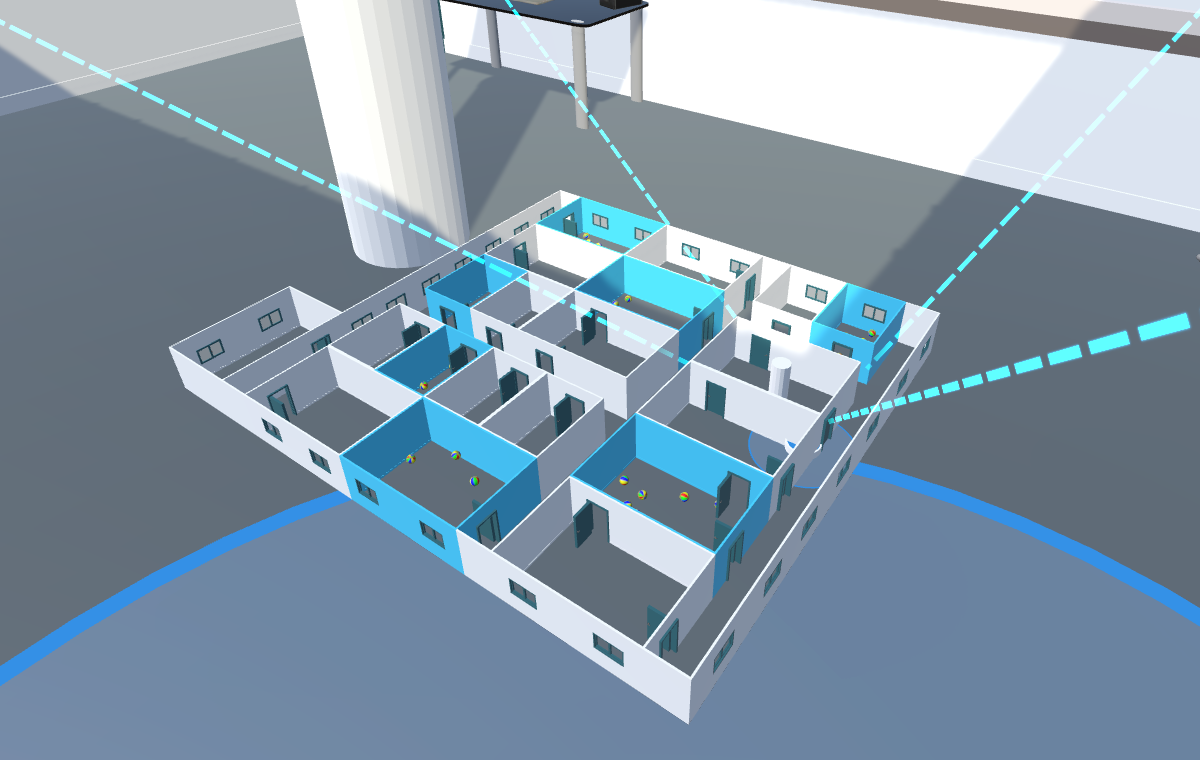
\includegraphics[width=\linewidth]{figures/screenshots/condition_3d_l_x}
    \caption{Beispiel des finalen Megamap-Prototypen in der Übersicht.}
    \label{fig:megamap_overview}
\end{figure}

\section{Unity Engine}
\emph{Unity} \autocite{UnityTechnologies2018} ist eine \emph{Engine} zum Entwickeln von 2D- und 3D-Anwendung (vornehmlich Spiele).
Da Unity plattformunabhängig ist werden die Applikationen gleichzeitig für mehrere Plattformen entwickelt.
Erstellt werden die Anwendungen mit dem Unity Editor.

Eine Unity-Anwendung ist in Szenen unterteilt.
Jede Szene besitzt einen eigenen Szenengraph.
Dieser Graph verwaltet alle Objekte einer Szene.
Unity verwendet ein Entitäten-Komponenten-System.
Das heißt, alle Unity-Objekte sind im Kern attribut- und funktionslose Entitäten (in Unity \emph{GameObject}s genannt).
Die eigentliche Funktionalität wird erst durch Hinzufügen von Komponenten (\emph{Components}) zu den GameObjects deutlich.
Beispielsweise verfügt das GameObject eines Würfel-Objekts über die Komponenten \lstinline{Transform} (Position, Rotation und Skalierung), \lstinline{MeshRenderer} (Geometrie) und \lstinline{BoxCollider} (Kollision).
Neben Anwendungen für den Desktop oder mobile Endgeräte bietet Unity native Unterstützung für eine Vielzahl an AR- und VR-Plattformen an \parencite{UnityTechnologies2018b}.

Zusätzlich zu diesen vorgefertigten Komponenten können auch Skript-Komponenten zu den GameObjects hinzugefügt werden.
Dies ermöglicht Entwicklern, komplett neues Verhalten für Objekte in die Engine zu integrieren.
Die Skripte werden in C\# oder einem Javascript-Dialekt geschrieben.
Die Skripte erben von der Unity-Klasse \lstinline|MonoBehaviour|, wodurch sie in den Lebenszyklus von Unity-Objekten aufgenommen werden und Eventmethoden wie z.B. \lstinline|Start()|, \lstinline|Update()|, \lstinline|FixedUpdate()| usw. erhalten \parencite{UnityTechnologies2018c}.

Eine Besonderheit bei Unity im Vergleich zu anderen Engines sind die \emph{Prefabs}.
Dabei handelt es sich um abgespeicherte Konfigurationen von GameObjects inklusive derer Komponenten.
Die Prefabs können dann jederzeit als vorkonfiguriertes Objekt instanziiert werden.
Darüber hinaus lässt sich Unity durch das Importieren von Plugins erweitern.
So werden \emph{Assets} (Texturen, Fonts, Musik, Materialien, Skripte) und Prefabs von anderen Entwicklern in das aktuelle Projekt übernommen.
Aufgrund der einfach zu nutzenden AR-/VR-Funktionalität sowie der Erweiterbarkeit wird Unity für diese Arbeit eingesetzt.

\section{SteamVR Plugin}
Ein nennenswertes Plugin, was für diese Arbeit eingesetzt wird, ist das \emph{SteamVR Plugin} \autocite{ValveCorporation2018}.
Dieses baut die in Unity integrierte AR-/VR-Unterstützung weiter aus.

Eine zentrale Rolle nimmt das \emph{Player}-Prefab ein.
Durch Platzieren dieses Prefabs in der Unity-Szene werden automatisch GameObjects erzeugt, welche die Positionen und Rotationen vom HMD und weiteren Controllern eines verbundenen VR-Systems tracken.
Die Zuordnung der Geräte zu den GameObjects ist hardware-übergreifend und geschieht automatisch.
Zudem wird dem Nutzer eine Begrenzung des Spielebereichs angezeigt, welche sich aus der verwendeten Technologie ergibt (in diesem Fall die sationären \emph{Lighthouse} Basisstationen der Vive).
Ebenso werden 3D-Modelle der Hand angezeigt, wobei sich die Finger der virtuellen Hände zu den Knöpfen bewegen, die der Nutzer aktuell betätigt.
Das Prefab übernimmt außerdem das stereoskopische Rendern, sodass auf dem HMD für jedes Auge ein anderes Bild angezeigt wird, wodurch der Eindruck von räumlicher Tiefe entsteht.

Für diese Arbeit wird außerdem das \lstinline{Interactable}-SteamVR-Skript verwendet.
Durch dieses Skript können GameObjects mit einer \lstinline{Collider}-Komponente auf die virtuellen Hände bzw. Controller reagieren und interaktive gemacht werden (z.B. Aufnehmen und werfen von Objekten, anklicken von Knöpfen etc.).
Die Verwendungen dieses Skripts für den Megamap-Prototypen werden an entsprechender Stelle in den folgenden Abschnitten näher beschrieben.

\section{Virtuelle Laborumgebung}
Wie eingangs in \autoref{sec:motivation_ziel} erwähnt war die ursprüngliche Idee dieser Arbeit die Implementierung eines Megamap-Prototypen für das MR-HMD Magic Leap One.
Dabei sollte die virtuelle Karte mithilfe des HMDs in die reale Umgebung des Nutzers integriert werden.

Zu Beginn der Arbeit war allerdings statt der MR-Hardware nur ein Software-Simulator als Entwicklervorschau verfügbar.
Im Verlauf der Arbeit wurde die MR-Hardware veröffentlicht.
Das HMD war in der Arbeitsgruppe Human-Computer~ Interaction der Universität Bremen jedoch weiterhin nicht verfügbar.
Daher wurde in dieser Arbeit ein alternativer Prototyp für das VR-HMD HTC Vive entwickelt.
Wie die meisten VR-HMDs verdeckt die Vive das Sichtfeld des Nutzers komplett, um stattdessen die virtuellen Inhalte anzuzeigen.
Somit ist die reale Welt für die Nutzer nicht mehr sichtbar, was die visuelle Integration der Megamap in Umgebung unmöglich macht.

Der entwickelte Prototyp umgeht dieses Problem, indem ein virtuelles Modell der Umgebung im Maßstab 1:1 verwendet wird.
So wird die reale Welt um den Nutzer herum virtuell simuliert.
Die virtuelle Megamap kann dann in die \textit{virtuelle} Umgebung des Nutzers integriert werden.
Die Idee hinter diesem Ansatz ist, dass durch die Ähnlichkeit der realen und der virtuellen Umgebung das Prinzip des VR-Prototypen auf eine Situation mit einem MR-HMD weiterhin übertragbar ist.
In zukünftigen Arbeiten könnte damit der Megamap-Prototyp auf MR-HMDs eingesetzt werden, ohne grundlegende Änderungen vornehmen zu müssen.
Durch die Verwendung eines 3D-Modells wird außerdem die 3D-Rekonstruktionsfunktion der Magic Leap One nachgeahmt.
Wie auch die HoloLens erstellt die Magic Leap One durch aktives Tracking der Umwelt intern ein 3D-Modell der Umgebung.
Dieses wird für die Kollisionsberechnung mit den virtuellen Inhalten verwendet.
So können virtuelle Objekte mit realen Gegenständen interagieren (z.B. läuft ein Charakter über einen realen Tisch oder ein virtueller Bildschirm wird an einer realen Wand platziert).
Durch die Verwendung eines 3D-Modells der Umgebung im Megamap-Prototypen ist Möglichkeit der Interaktion mit der Umwelt implizit gegeben.

Für den Prototypen wurde ein maßstabsgetreues 3D-Modell des Laborraums der Arbeitsgruppe Human-Computer~ Interaction der Universität Bremen angefertigt, welcher der Ort der durchgeführten Nutzerstudie ist (siehe \autoref{chap:evaluation}).
\autoref{fig:lab_environment} zeigt ein Foto des Laborraums sowie Screenshots der entsprechenden virtuellen Umgebung.
Der Grundriss des Raums wurde im Modellierungsprogramm \emph{Blender} mithilfe des eingebauten \emph{Archimesh}-Werkzeugs zentimetergenau erstellt.
Das Modell wurde als \texttt{.fbx} in Unity importiert und mit diversen virtuellen Requisiten ergänzt, um den Raum realistischer und dem Original ähnlicher wirken zu lassen.
\begin{figure}[thb]
    \begin{subfigure}{0.49\textwidth}
        \centering
        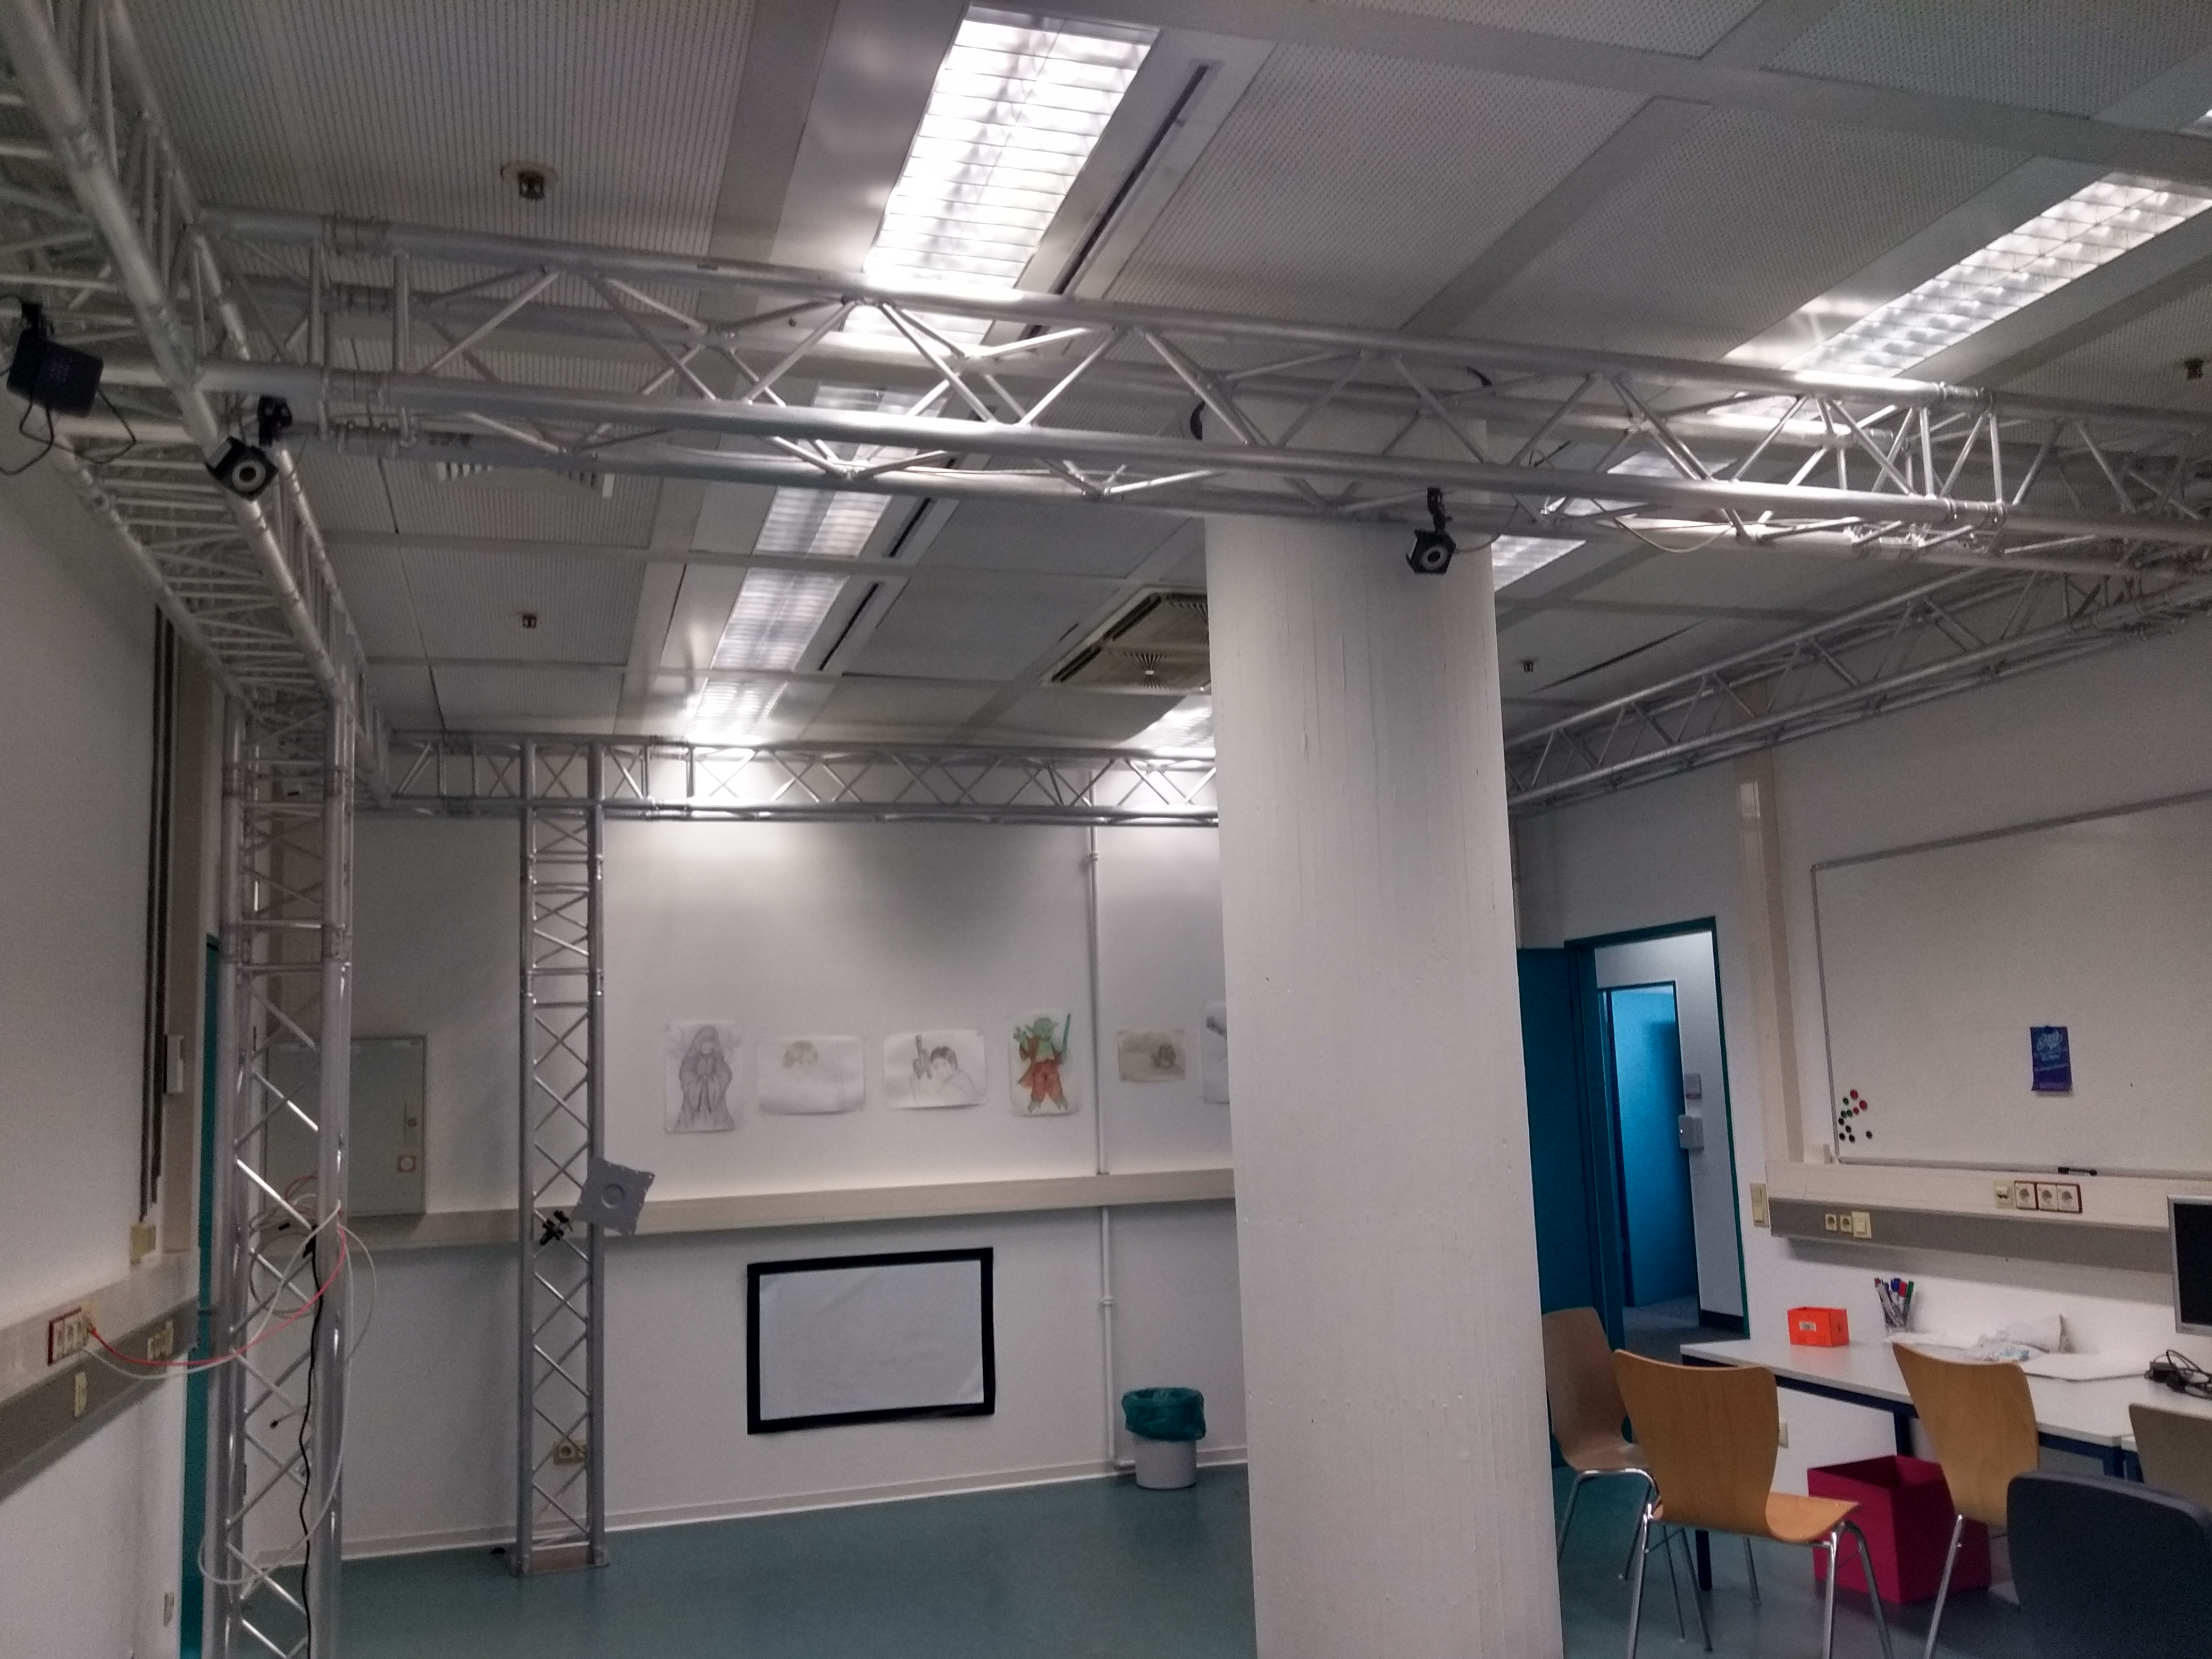
\includegraphics[width=0.755\textwidth]{figures/photo_lab}
        \caption{}
        \label{sfig:lab_photo}
    \end{subfigure}
    \hfill
    \begin{subfigure}{0.49\textwidth}
        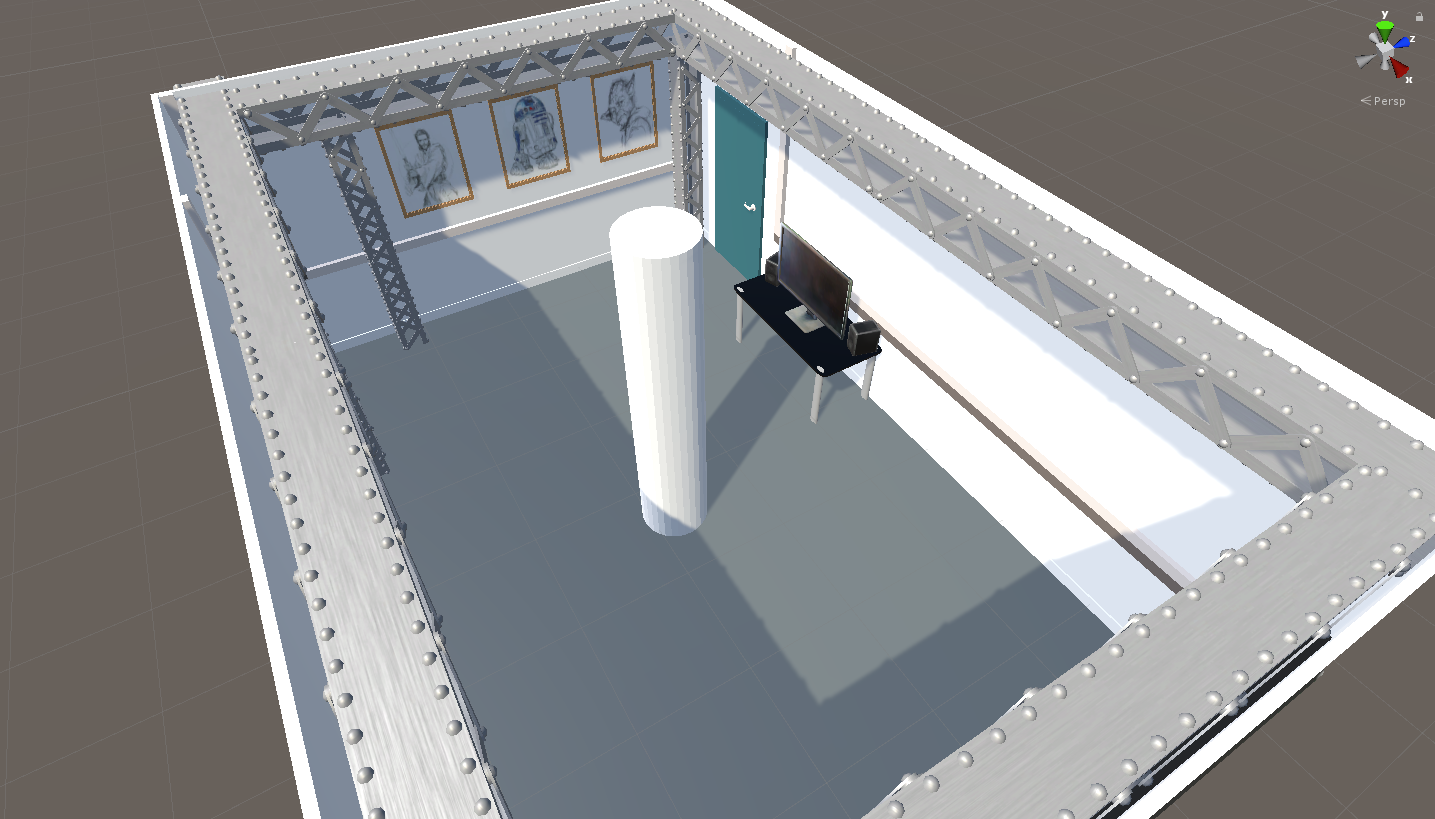
\includegraphics[width=\textwidth]{figures/lab3}
        \caption{}
        \label{sfig:lab_screenshot_1}
    \end{subfigure}

    \vspace{1em}
    \begin{subfigure}{0.49\textwidth}
        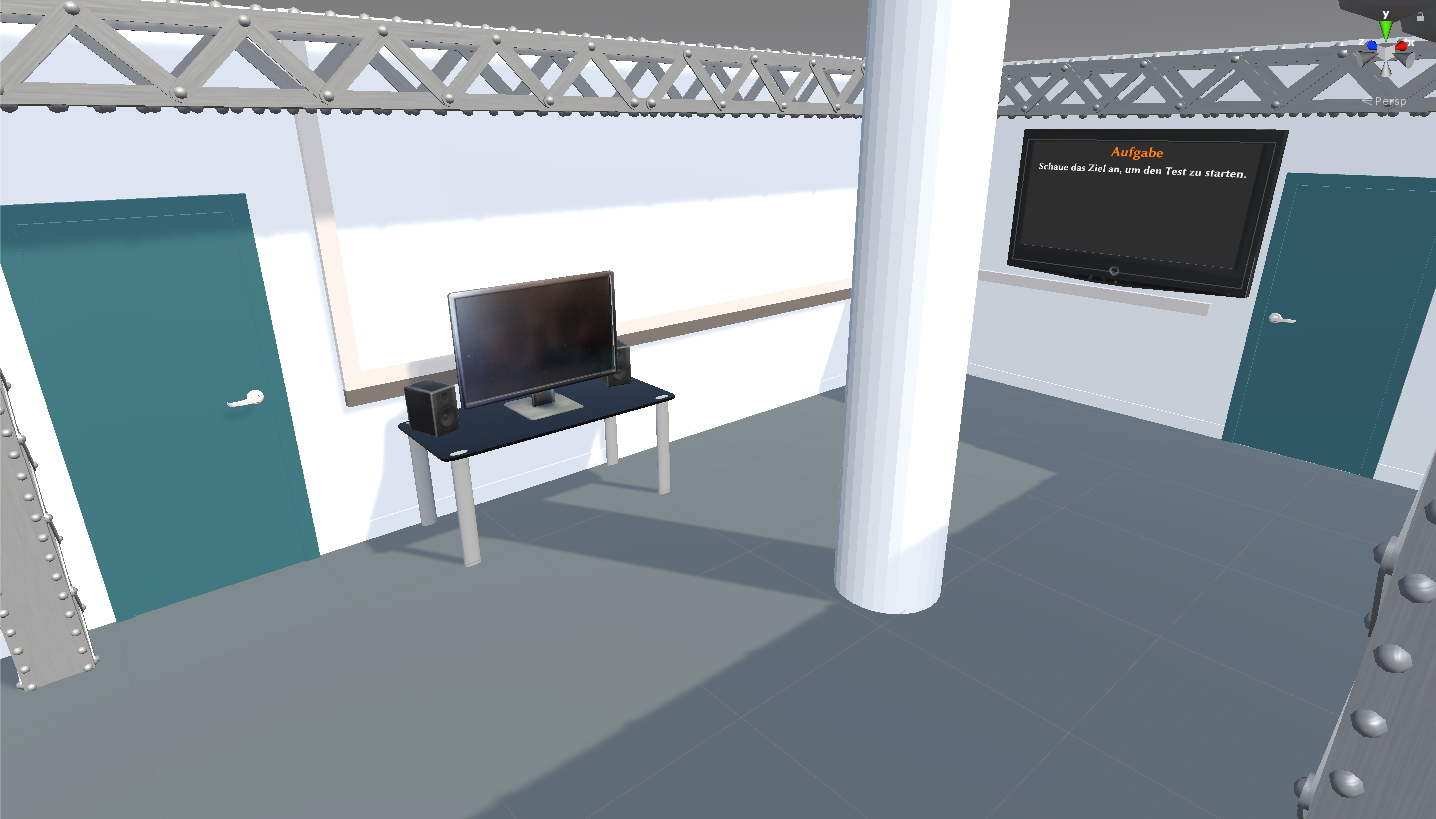
\includegraphics[width=\textwidth]{figures/lab1}
        \caption{}
        \label{sfig:lab_screenshot_2}
    \end{subfigure}
    \hfill
    \begin{subfigure}{0.49\textwidth}
        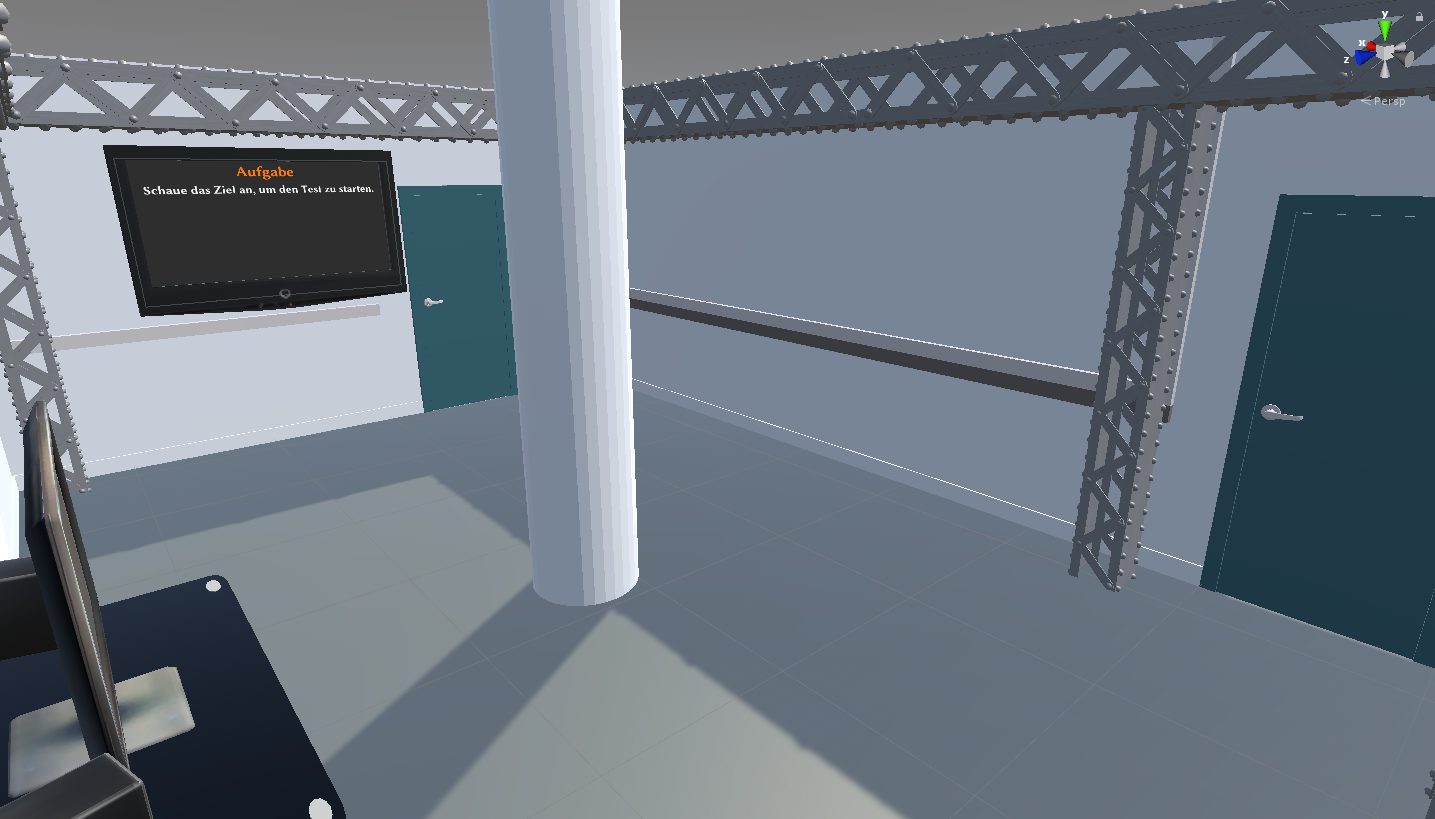
\includegraphics[width=\textwidth]{figures/lab2}
        \caption{}
        \label{sfig:lab_screenshot_3}
    \end{subfigure}
    \caption{Um die Situation der MR-Anwendung in VR nachzubilden, wurde der Laborraum im Maßstab 1:1 modelliert. %
             (\subref{sfig:lab_photo}) Foto des realen Laborraums. %
             (\subref{sfig:lab_screenshot_1})--(\subref{sfig:lab_screenshot_3}) Screenshots des virtuellen Laborraums in Unity.%
	}
	\label{fig:lab_environment}
\end{figure}

\subsection*{Synchronisation der realen und virtuellen Position}
Damit die virtuelle Umgebung als Ersatz für die reale Umgebung verwendet werden kann muss sichergestellt werden, dass die Rotation des virtuellen Raums der des realen Raums entspricht \emph{und} dass die Position des Nutzers in der virtuellen Welt seiner Position in der realen Welt entspricht.
Der Prototyp muss dafür vorab in zwei Schritten konfiguriert werden:

\paragraph{Erster Schritt:}
Während der Kalibrierung der Vive legt der Nutzer den Spielebereich (die sogenannte \emph{Play Area}) fest.
Dies ist der Bereich, in dem sich keine Hindernisse für den Nutzer befinden und der für die Basisstationen sichtbar ist.
Hierfür zieht der Nutzer mit den Controllern ein Rechteck nach, welches dann als Spielebereich gesetzt wird.
Es wichtig, dass die längere Seite des Rechtecks orthogonal zur Ausgangsrotation des \lstinline{Player}-Objekts in Unity verläuft.
Die aktuell getrackte Rotation des HMDs wird relativ zur Ausrichtung der Play Area gemessen.
Da SteamVR automatisch die längeren Seiten der Play Area als Vorder- bzw. Rückseite betrachtet, müssen diese orthogonal zur Blickrichtung des \lstinline{Player}-Objekts verlaufen.
Im Fall des entwickelten Prototypen bedeutet dies, dass die Vorderseite der Play Area parallel zu der Wand des Labors verlaufen muss, an der sich die Eingangstür und Tische befinden (siehe \autoref{fig:lab_environment}).
Die korrekte Kalibrierung der Play Area wird in \autoref{fig:ve_setup_correct} skizziert.
Wenn bei der Kalibrierung der Play Area eine andere Ausrichtung gewählt wird, als die Ausgangsrotation des \lstinline{Player}-Objekts, weicht die virtuelle Rotation des Nutzers von der realen Rotation im Bezug zum Raum ab.
Effektiv hätte die virtuelle Umgebung dann eine andere Ausrichtung als die reale Umgebung.
Die falsche Kalibrierung wird in \autoref{fig:ve_setup_wrong} dargestellt.

Ginge es nur um den visuellen Reiz in der virtuellen Umgebung, würde der Nutzer diese Abweichung lediglich beim Aufsetzen des HMDs bemerken (da dann der virtuelle Raum anders rotiert wäre als der reale).
Wenn aber zum Beispiel der Tastsinn eine Rolle spielt, dann ist eine korrekte Ausrichtung des virtuellen Raums sinnvoll.
Da in dem entwickelten Prototyp nicht ausgeschlossen ist, dass der Nutzer die Play Area verlässt und beispielsweise die Säule oder Wände mit den Händen berührt, ist es für die Immersion von Vorteil, wenn das Berühren der virtuellen Objekte mit den taktilen Reizen der realen Objekte verknüpft wird.
Weiterhin wird durch die korrekte Ausrichtung die Messung des Abweichungsfehlers beim Zeigen auf Objekte erleichtert, was detailliert in \autoref{chap:evaluation} beschrieben wird.

\begin{figure}
    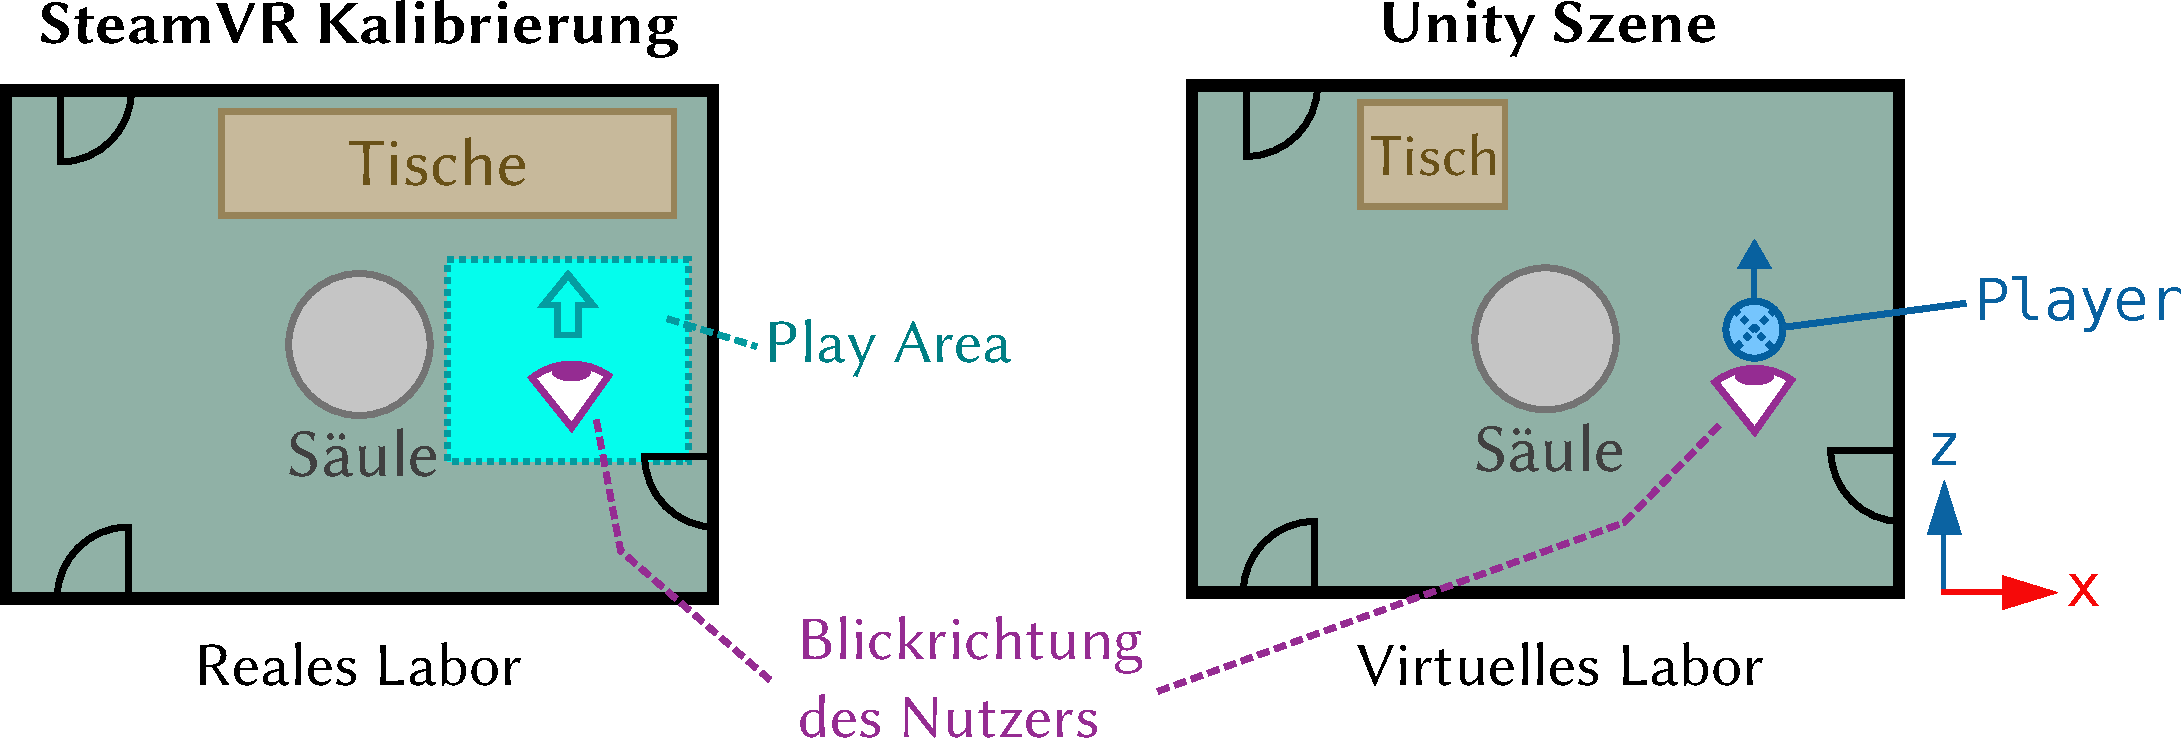
\includegraphics[width=\textwidth]{figures/environment_setup_correct}
    \caption{Die Play Area hat die gleiche Ausrichtung wie das \lstinline{Player}-Objekt in der Grundrotation (entlang z-Achse). %
    Die Rotation des Nutzers in der realen und virtuellen Welt stimmt überein.}
    \label{fig:ve_setup_correct}
\end{figure}

\begin{figure}
    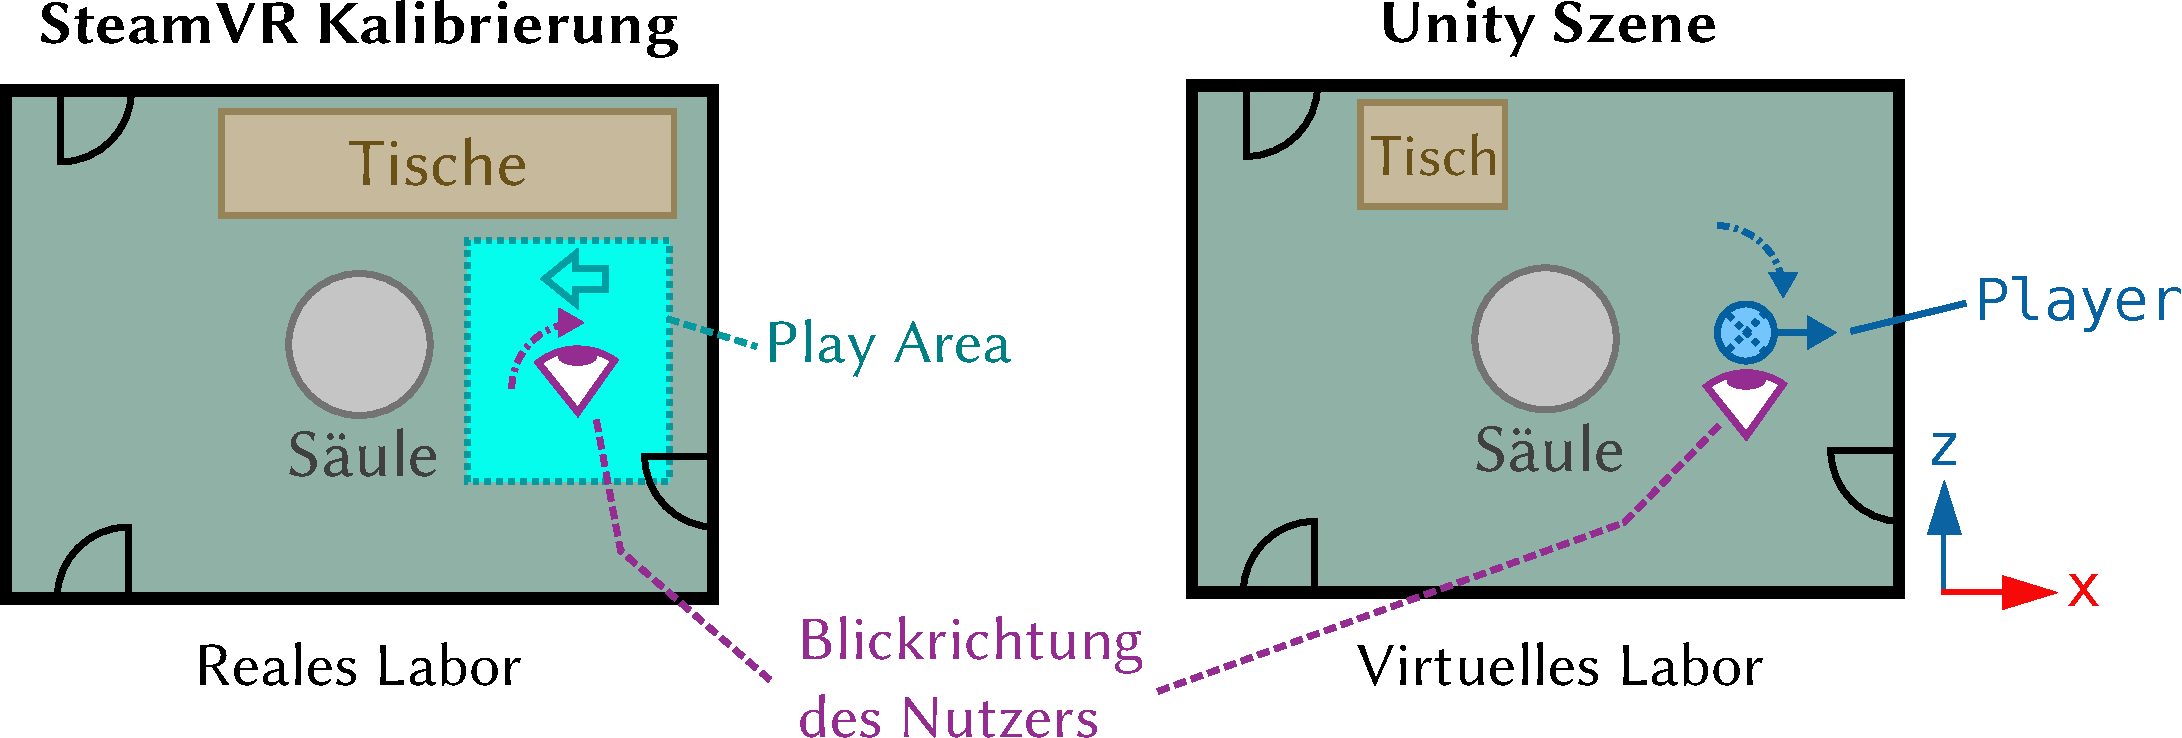
\includegraphics[width=\textwidth]{figures/environment_setup_wrong}
    \caption{Die Play Area hat \emph{nicht} die gleiche Ausrichtung wie das \lstinline{Player}-Objekt in der Grundrotation. %
        Der Nutzer hat einen Rotationsoffset (hier \ang[detect-weight=true]{90}), wodurch für den Nutzer effektiv die Räume unterschiedlich rotiert wirken.}
    \label{fig:ve_setup_wrong}
\end{figure}

\paragraph{Zweiter Schritt:}
Neben der Orientierung des Nutzers muss die Position des virtuellen Raums angepasst werden, wenn dieser die reale Umgebung bestmöglich überlagern soll.
Dies resultiert (wie bei der Rotation) aus der Tatsache, dass die getrackte Position des HMDs im Bezug zur Play Area gemessen wird, welche sich durch den Kalibrierungsvorgang von SteamVR ändern kann.
Um neue Position des virtuellen Raums zu bestimmen wird für den Prototypen wie folgt vorgegangen:

Der Prototyp wird mit seiner Ausgangsposition im Unity Editor ausgeführt.
Die Ecke \enquote{links unten} aus Vogelperspektive des virtuellen Labors befindet sich an der Unity-Welt-Koordinate $(0, 0, 0)$.
Die Controller, welche im HMD durch 3D-Modelle visualisiert sind, werden in den Ecken des virtuellen Raums platziert.
Dabei wird darauf geachtet, dass sie von den Basisstationen weiterhin erkannt werden.
Nun wird im realen Labor die Entfernung von den Controllern zu den entsprechenden Ecken des Raums gemessen, was der Abweichung der virtuellen Welt entspricht.
Die Entfernungen werden gemittelt.
Der resultierende Offset wird dann im Unity Editor verwendet, um das virtuelle Labor zu verschieben.
Dieser Offset ist nun solange gültig, bis die Play Area neu kalibriert wird.
Wie auch schon bei der Rotation ist diese Angleichung erst dann für die Nutzer bemerkbar, wenn sie versuchen physische Objekte wie Wände oder die Säule zu berühren.
Würde die Verschiebung des Raums nicht durchgeführt werden, könnten Nutzer mit den Controllern durch die virtuellen Objekte hindurch greifen oder sie würden auf physische Barrieren stoßen, obwohl die virtuellen Objekte noch weiter entfernt sind.
Nach diesen beiden Schritten kann der virtuelle Raum als Ersatz für die reale Umgebung verwendet werden, die in einer MR-Anwendung ohne vorheriges Modellieren verfügbar wäre.

\section{Das Megamap-GameObject}
\begin{figure}[t]
    \centering
    \imagebox{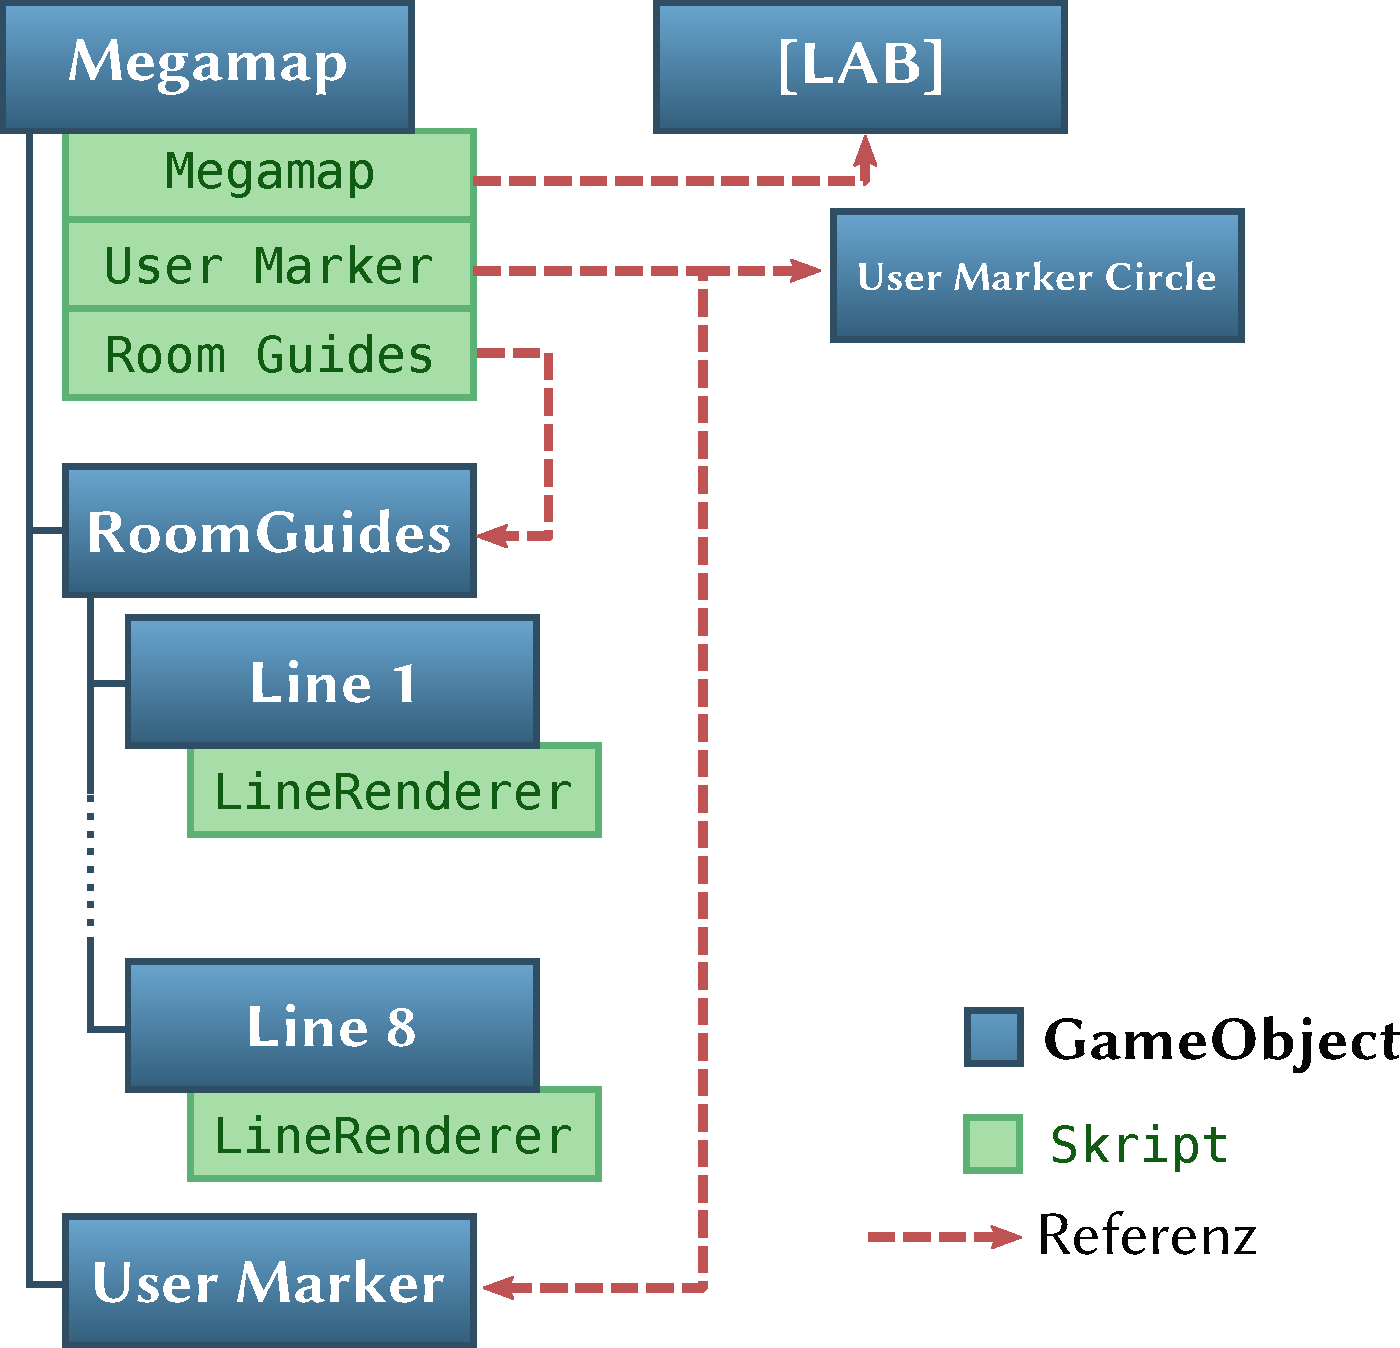
\includegraphics[height=8.5cm]{figures/unity_megamap_object}}
    \caption{Übersicht des Megamap-GameObjects.}
    \label{fig:unity_megamap_object}
\end{figure}

Eine grundlegende Implementierung des in \autoref{chap:concept} vorgestellten Megamap-Konzepts wird im Megamap-GameObject realisiert.
Eine strukturelle Übersicht des Objekts wird in \autoref{fig:unity_megamap_object} gegeben.
Das Objekt setzt sich aus drei Teilen zusammen, die jeweils durch eigene Komponenten repräsentiert werden:

Das Skript \textbf{\lstinline{Megamap}} bietet allgemeine Einstellungsmöglichkeiten zur Darstellung der Megamap.
Es lassen sich z.B. die Skalierung oder die Höhe vom Boden ändern.
Weiterhin bietet das Skript die Methoden \lstinline{Show()} und \lstinline{Hide()}, mit denen die Karte angezeigt bzw. ausgeblendet werden kann.
Falls dabei das Feld \lstinline{useAnimation} auf \lstinline{true} gesetzt ist, wird die Karte beim Anzeigen von einer 1:1 Raumgröße auf die eingestellte Skalierung nach und nach herunterskaliert (beim Ausblenden analog ein Hochskalieren).
Die Megamap wird standardmäßig Nutzer-zentriert platziert.
Das bedeutet, dass der Nutzer sowohl in der realen Welt als auch auf der Karte die gleiche Position einnimmt.
Hierfür wird die virtuelle Umgebung referenziert und der Abstand vom HMD zum Ursprung des Labor-Modells ermittelt.
Dieser Abstand wird dann wie die Megamap skaliert und die Karte wird um den skalierten Abstand verschoben.
Sowohl die Animation als auch die Zentrierung auf den Nutzer sollen es ihm erleichtern, seine eigene Position auf der Karte zu finden.
Außerdem soll hierdurch der Bezug vom Laborraum auf der Karte zum umgebenden Laborraum hervorgehoben werden.

Das \lstinline|Megamap|-Skript dient lediglich als Schnittstelle zur Manipulation der Karte.
Das eigentliche 3D-Modell, welches als Karte verwendet wird, ist von diesem Skript unabhängig und wird erst zur Laufzeit durch andere Skripte als aktive Karte gesetzt.
Hierfür bietet das \lstinline|Megamap|-Skript die Methode \lstinline|SetMap(...)| an, welche als Parameter unter anderem eine Referenz auf ein \lstinline|IndoorMap|-Skript erwartet.
Dank dieser Trennung von Schnittstelle und Modell können zur Laufzeit unterschiedliche Indoor-Karten gewechselt werden, was für die Nutzerstudie in \autoref{chap:evaluation} Voraussetzung ist.
Die Details zum \lstinline|IndoorMap|-Skript werden in \autoref{sec:indoor_maps} ausgeführt.

\begin{figure}
    \centering
    \begin{minipage}[t]{.485\textwidth}
        \centering
        \vspace{0pt}
        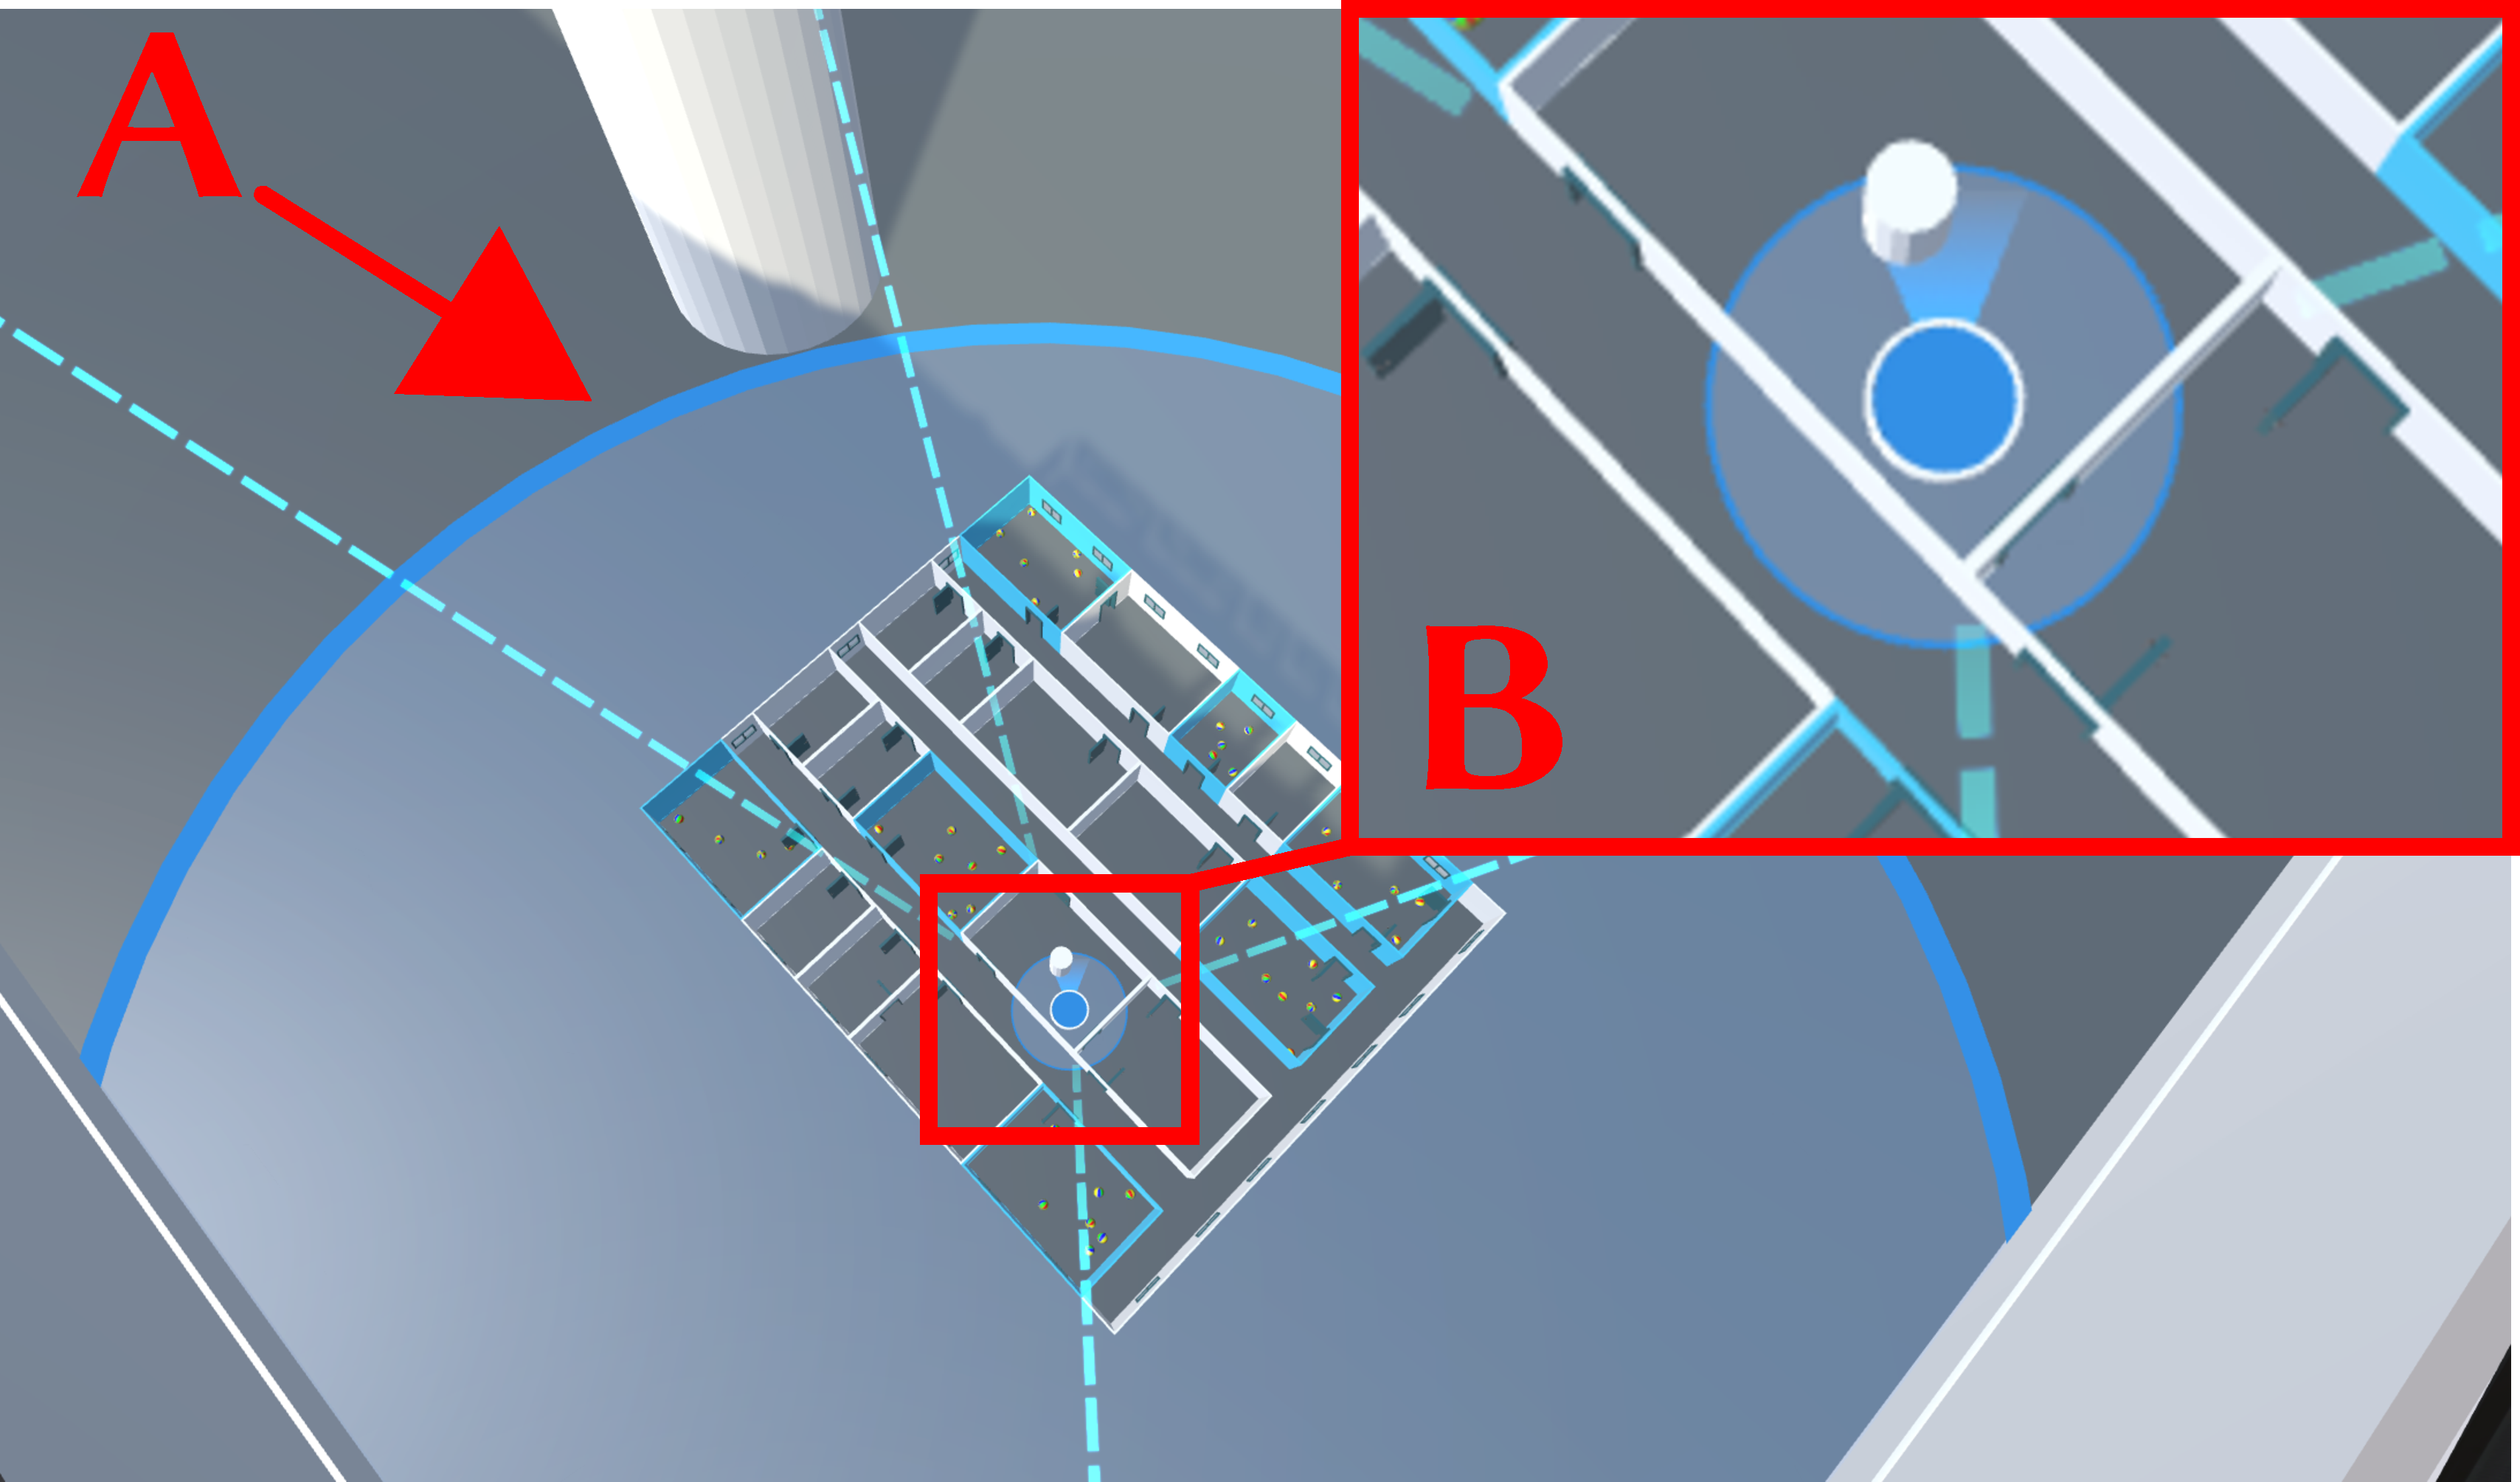
\includegraphics[width=\linewidth]{figures/megamap_user_marker.pdf}
        \captionof{figure}{Der User Marker zeigt die Position des Nutzers auf der Megamap an. %
            \textcolor{red}{A:} Marker in Umgebung. %
            \textcolor{red}{B:} Marker auf Karte.%
        }
        \label{fig:user_marker}
        \vfill
    \end{minipage}
    \hfill
    \begin{minipage}[t]{.485\textwidth}
        \centering
        \vspace{0pt}
        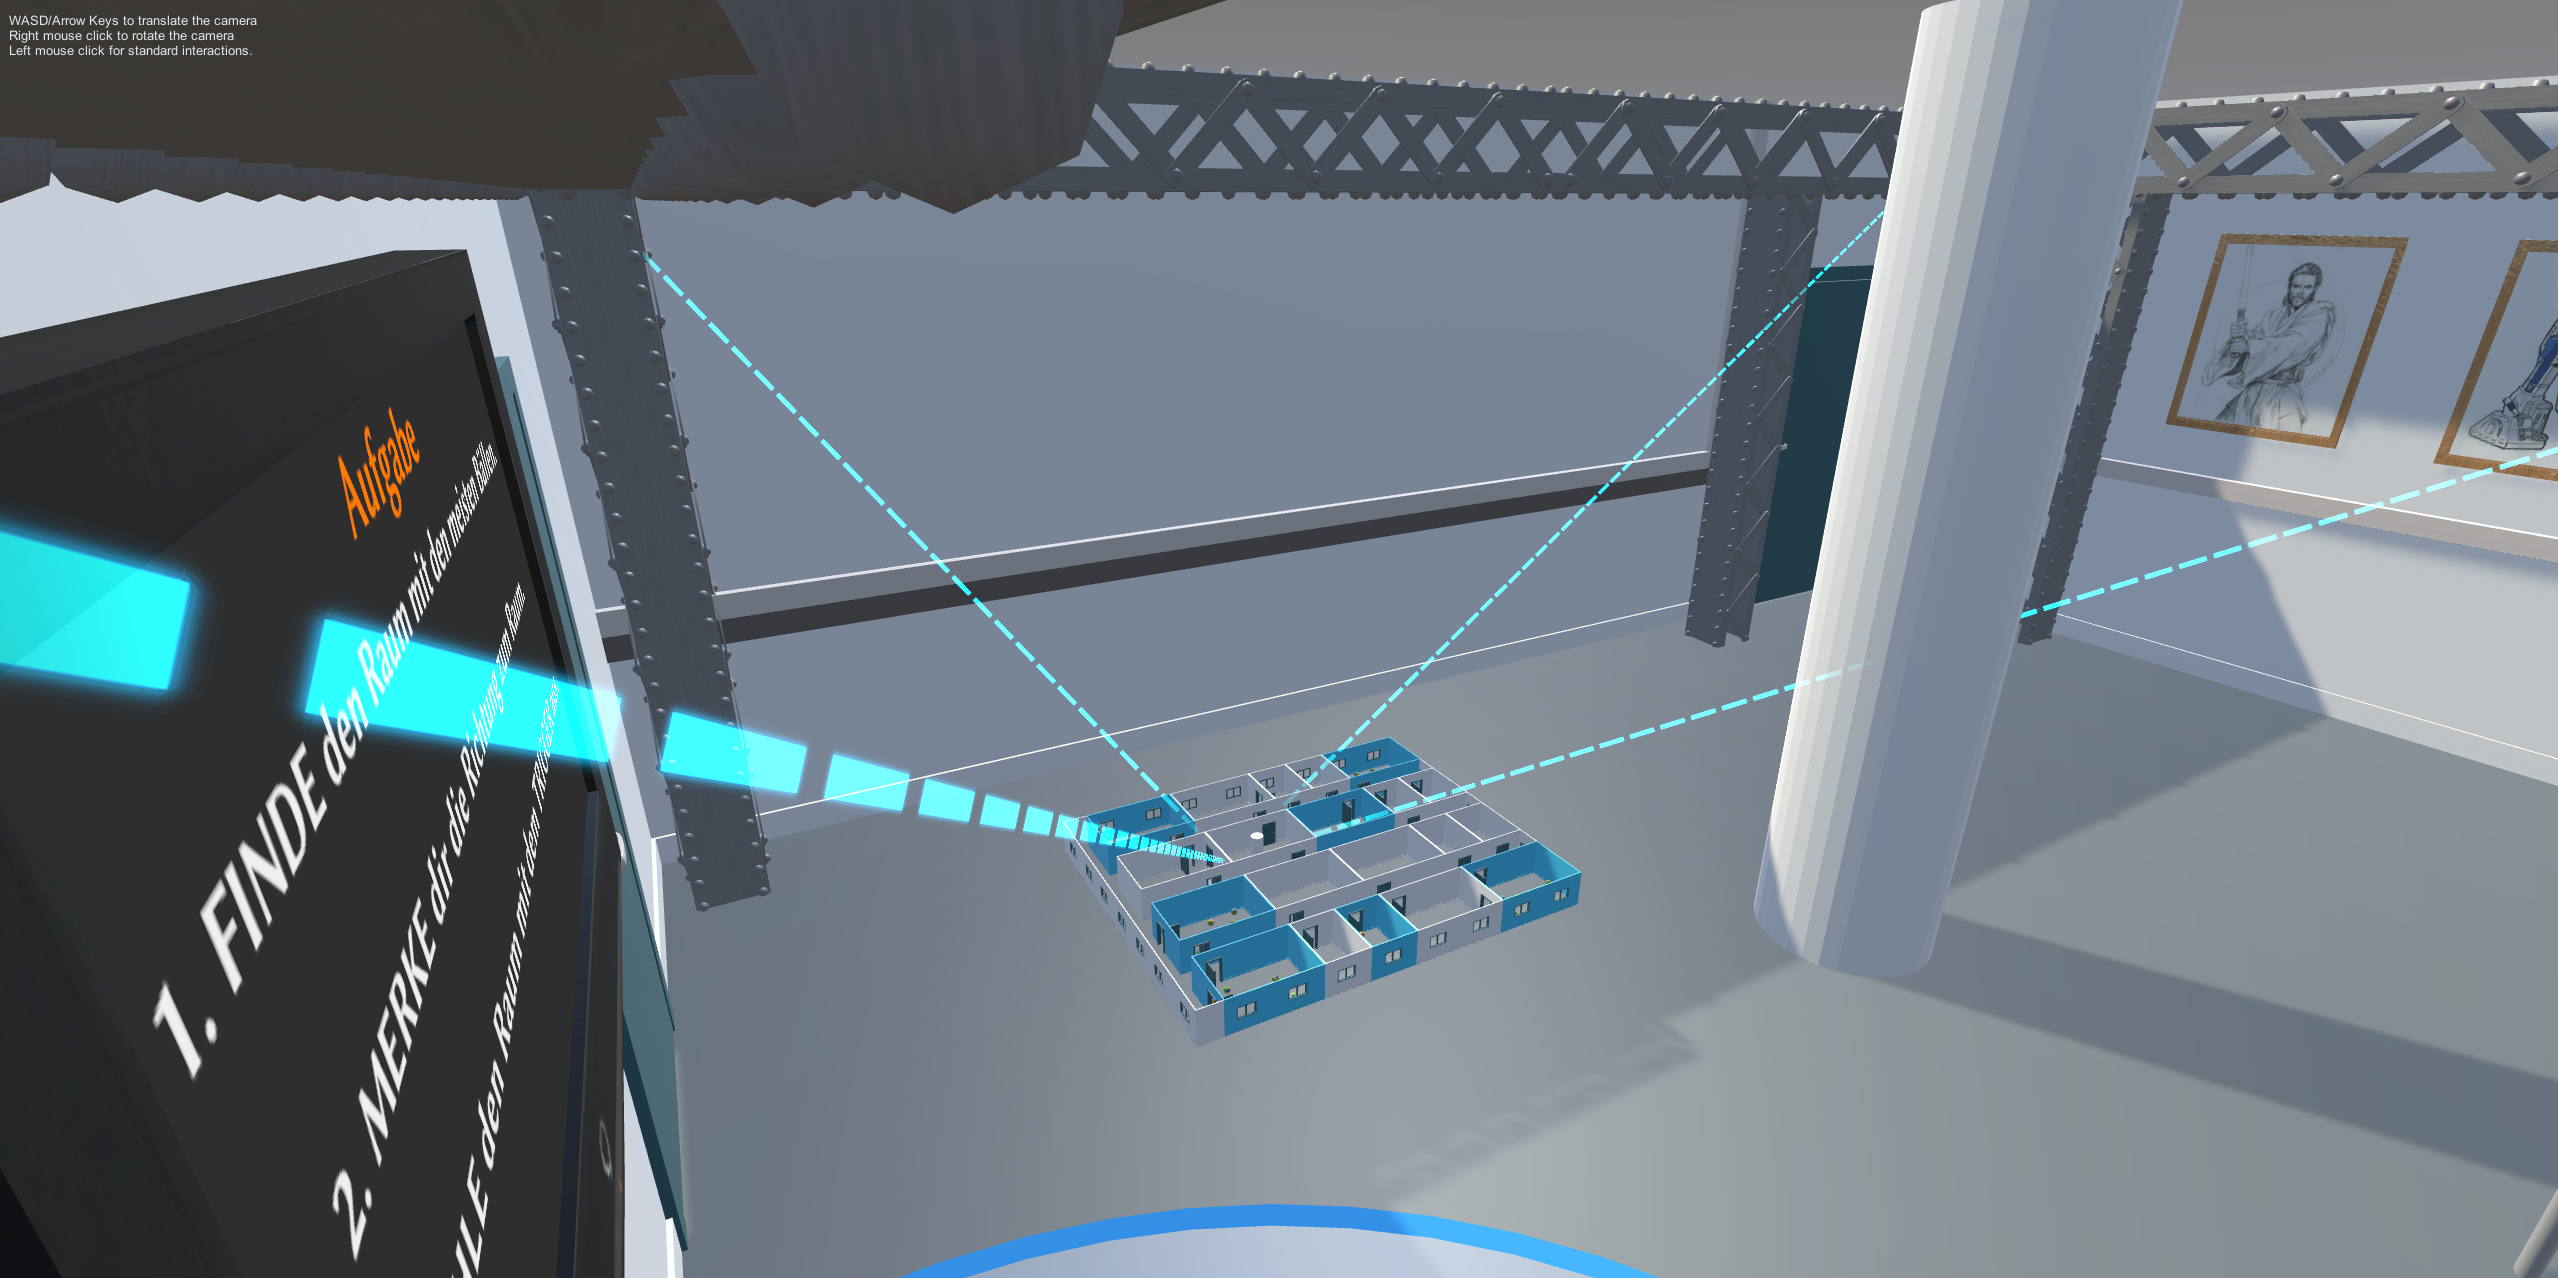
\includegraphics[width=\linewidth, height=4.2cm]{figures/megamap_room_guides}
        \captionof{figure}{Die Room Guides verbinden die Ecken des umgebenden Raums mit dem entsprechenden Raum auf der Megamap.}
        \label{fig:room_guides}
    \end{minipage}
\end{figure}

Der zweite Teil des Megamap-Objekts, das \textbf{\lstinline|User Marker|} Skript, dient ebenfalls der Orientierung für den Nutzer.
Analog zu Kartenanwendungen wie Google Maps befindet sich ein Marker auf der Megamap, welcher die aktuelle Position des Nutzers anzeigt.
Da es sich bei der Megamap um eine dreidimensionale Karte handelt wird hier ein Zylinder in Form ähnlich eines Pucks benutzt (siehe \autoref{fig:user_marker}).
Mittels eines transparenten Kreissegments wird außerdem die aktuelle Rotation des Nutzers verdeutlicht.
Um den Bezug vom Marker auf der Karte zur Umgebung zu verstärken ist auch in dieser ein Kreis platziert, welcher auf dem Nutzer zentriert ist.

Der dritte Teil des Megamap-Objekts ist das \textbf{\lstinline|Room Guides|} Skript.
Durch dieses werden Linien von den Ecken des umgebenden Laborraums zum Laborraum auf der Karte gezogen (siehe \autoref{fig:room_guides}).
Die Linien heben den Raum hervor, in dem sich der Nutzer befindet und stellen somit einen Bezug zur Umgebung her.
Implementiert sind diese Führungslinien als acht \lstinline|GameObject|s mit jeweils einer \lstinline|LineRenderer|-Komponente, die zusammen mit der Megamap ein- bzw. ausgeblendet werden.
Für die Startpunkte der Linien (die Ecken des umgebenden Raums) wird über die \lstinline|Renderer|-Komponente des Labor-Modells auf dessen \emph{Bounding Box} zugegriffen.
Die Eckpunkte der Bounding Box sind die Startpunkte der Linien.
Die Endpunkte der Linien werden berechnet, indem die Startpunkte mit der Transformationsmatrix der Megamap multipliziert werden.
So entsteht der Effekt, dass die Linien zu den Eckpunkten des Labors auf der Karte hinführen.
Standardmäßig werden über das Feld \lstinline|showUpperOnly| nur die oberen vier Linien angezeigt, da die unteren Führungslinien vom Rest der Megamap verdeckt werden würden.

\section{Erstellung der Indoor-Karten}
\label{sec:indoor_maps}
Wie bereits erwähnt ist das eigentliche 3D-Modell, welches das Layout des Gebäudes repräsentiert, vom \lstinline|Megamap|-Skript getrennt.
Für den in dieser Arbeit entwickelten Prototypen werden vorab erstellte 3D-Modelle eingesetzt, die in Blender mit dem Archimesh-Werkzeug modelliert wurden.
Ansätze zur automatisierten Generierung von Gebäudemodellen werden in \autoref{sec:building_data_automation} untersucht.

Die erstellten Karten sind 3D-Modelle, bei denen die einzelnen Räume als separate GameObjects in Unity verfügbar sind.
\autoref{fig:room_hierarchy} zeigt schematisch, wie die Objekthierarchie für die Indoor-Karten in Unity aufgebaut ist.

Für die Nutzerstudie aus \autoref{chap:evaluation} ist es notwendig, dass Nutzer mit Räumen interagieren können.
Es wird eine Suchaufgabe implementiert, bei der die Nutzer den Raum finden müssen, der die meisten Bälle enthält.
Die Nutzer können mit den Vive-Controllern Räume anvisieren und durch Betätigung des Triggers auswählen.
Handelt es sich um den gesuchten Raum, wird die Karte ausgeblendet.
Ansonsten wird der Raum als \enquote{falscher Raum} hervorgehoben.

\begin{figure}[tbh]
    \centering
    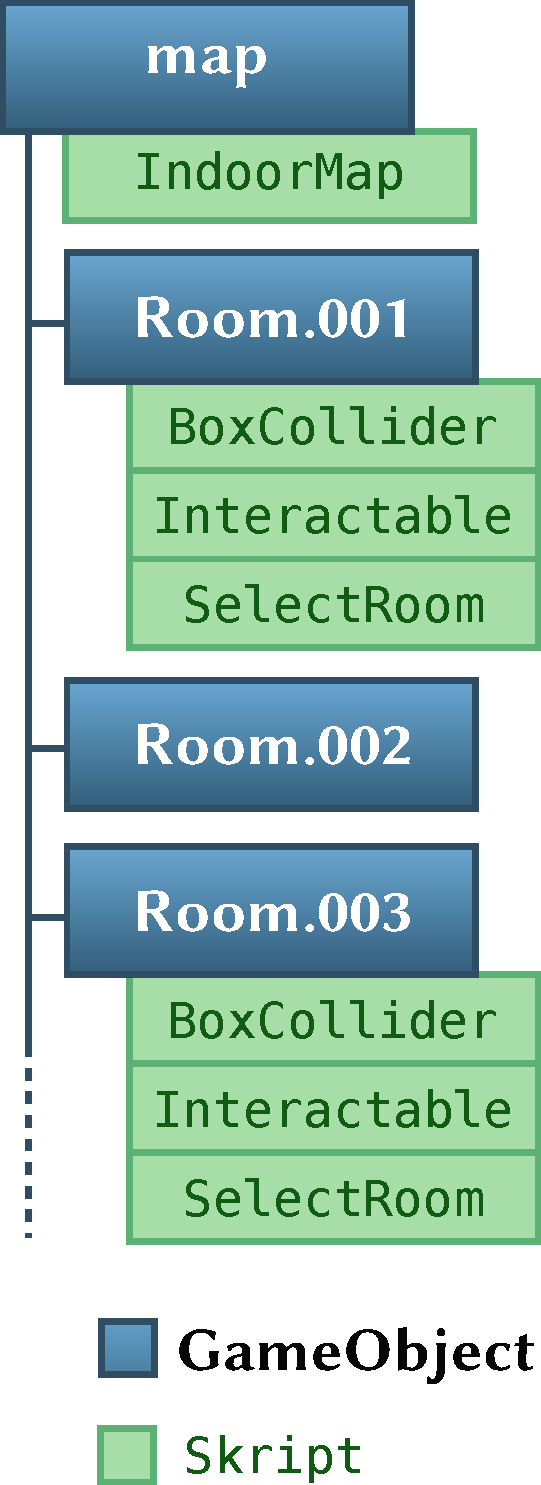
\includegraphics[height=9cm]{figures/unity_indoor_map}
    \caption{Objekthierarchie des IndoorMap-Objekts,}
    \label{fig:room_hierarchy}
\end{figure}

Diese Interaktionsmöglichkeit wird durch das \lstinline|SelectRoom|-Skript umgesetzt.
Das Skript verwendet die SteamVR-Komponente \lstinline|Interactable|, wodurch Räume auf An\-nä\-he\-rungs- und Interaktionsevents der Vive-Controller reagieren können.
Im Skript werden dazu spezielle SteamVR-Methoden implementiert.
Die Methode \lstinline|OnHandHoverBegin(...)| wird ausgelöst, sobald die \lstinline|HoverTransform| des Vive-Controllers den Collider des Raums berührt.
In der Methode wird der Raum gelb hervorgehoben, wenn er zuvor nicht angeklickt wurde.
Wenn er zuvor bereits angeklickt wurde (und nicht der gesuchte Raum ist) wird der Raum stattdessen rot eingefärbt.

Die Methode \lstinline|OnHandHoverEnd(...)| setzt die Farbe des Raums in den Normalzustand zurück, wenn der Vive-Controller den Collider des Raums verlässt.
Somit ist die farbliche Änderung nur sichtbar, solange der Raum mit dem Controller anvisiert wird.

Die \lstinline|HandHoverUpdate(...)|-Methode wird in jedem Update-Iteration von Unity ausgeführt, solange der Vive-Controller den Collider des Raums überlappt.
In der Methode wird überprüft, ob aktuell der Trigger des Controllers betätigt wird.
Sobald der Trigger vom Nutzer gedrückt wird, wird ein Event ausgelöst, was die Auswahl eines Raums signalisiert.
Handelt es sich dabei um den gesuchten Zielraum, wird das Event \lstinline|OnTargetRoomSelected| ausgelöst.
Dieses wird an anderer Stelle benutzt, um die Karte bei Auswahl des Zielraums auszublenden.
Wenn der falsche Raum gewählt wird, wird stattdessen das Event \lstinline|OnWrongRoomSelected| aktiviert.
Dieses wird genutzt, um die Auswahl von falschen Räumen zu zählen und in \autoref{chap:evaluation} auszuwerten. 

Um den Zugriff auf die Räume zu vereinfachen verfügt das IndoorMap-Objekt über das gleichnamige Skript \lstinline|IndoorMap|.
Dieses bietet C\#-Eigenschaften (\emph{Properties}) an, um die Liste aller Räume bzw. die Liste aller \emph{auswählbarer} Räume zu erhalten (\lstinline|Rooms| bzw. \lstinline|SelectableRooms|).

Damit die Megamap das IndoorMap-Objekt als Karte verwendet wird es an die Methode \lstinline|SetMap(...)| des \lstinline|Megamap|-Skripts übergeben.
Hierdurch wird das IndoorMap-Objekt zu einem Kind-Objekt der Megamap.
Die Skalierung und Translation der Megamap werden automatisch für das Kartenmodell übernommen.
Die Karte kann durch weitere Aufrufe von \lstinline|SetMap(...)| ausgetauscht werden.

\section{Interaktion mittels virtuellem Laserpointer}
Mit den \lstinline|SelectRoom|- und \lstinline|Interactable|-Skripten können Nutzer die Räume auf der Karte mit dem Vive-Controller auswählen.
Allerdings müssten sie sich (ohne weitere Maßnahmen) zu den einzelnen Räumen hinbewegen, um diese mit dem Vive-Controllern zu berühren und auszuwählen.
In informellen Vortests des Prototypen zeigte sich, dass die Bewegung zu den Räumen umständlich ist, wenn lediglich ein einzelner Raum gefunden werden soll.
Die Play Area der Vive schränkt die Bewegung der Nutzer zusätzlich ein, da außerhalb der Play Area mit Hindernissen gerechnet werden muss und das Tracking durch die Basisstationen ungenauer wird.

Für den aktuellsten Prototyp wurde daher eine Methode zur entfernten Auswahl von Räumen entwickelt.
Über einen virtuellen \enquote{Laser Pointer} können Nutzer mit den Vive-Controllern auf Räume zeigen und diese mit dem Trigger auswählen.
Der Screenshot in \autoref{fig:laserpointer_screenshot} zeigt ein Beispiel.
Das Skript \lstinline|LaserPointer| setzt dies um, indem es einen \lstinline|LineRenderer| aktiviert, welcher einen Lasterstrahl darstellt.
Der Strahl verläuft vom Controller geradeaus in die Szene.
In der Methode \lstinline|Update()| wird dann durch \lstinline|Physics.RaycastAll(...)| ein Schnitttest zwischen dem Strahl und Collidern in der Szene durchgeführt.
Falls ein Collider vom Strahl getroffen wird und der Collider zu einem der Räume gehört, wird der Schnittpunkt als Endpunkt des Laserstrahls gesetzt.
So entsteht der Effekt, dass der Laserstrahl nicht durch die Räume hindurchgeht.
\begin{figure}[htb]
    \centering
    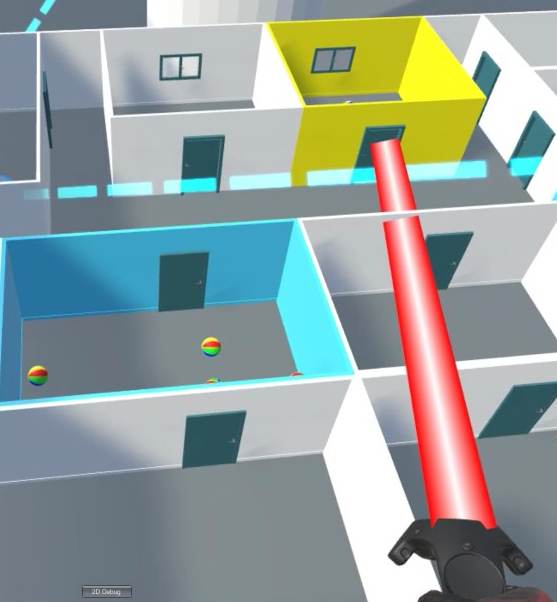
\includegraphics[height=6cm]{figures/screenshots/laserpointer}
    \caption{Mit dem Laserpointer wird ein Raum anvisiert.}
    \label{fig:laserpointer_screenshot}    
\end{figure}

Wie im vorigen Abschnitt beschrieben findet die Interaktion zwischen Vive-Controller und einem Raum statt, wenn der Controller den Raum überlappt.
Da jedoch beim Laserpointer der Controller vom Raum entfernt ist, muss hier eine Modifikation vorgenommen werden.
Intern nutzt das SteamVR-\lstinline|Hand|-Skript (welches den Controller repräsentiert und trackt) die Felder \lstinline|HoverSphereTransform| und \lstinline|HoverSphereRadius|.
Beide Felder definieren eine unsichtbare Kugel mit einem gegebenen Radius.
Standardmäßig folgt diese Kugel der Position des Controllers.
Sobald die Kugel mit einem \lstinline|Interactable|-Objekt überlappt, werden die entsprechenden SteamVR-Events ausgelöst.
Für den Laserpointer wird diese Kugel verschoben, wenn der Raycast einen Schnittpunkt mit einem auswählbaren Raum ergibt.
Die Position der Kugel wird auf den Schnittpunkt geändert, wodurch sie sich effektiv am Ende des Laserstrahls befindet.
Damit werden die SteamVR-Events für den entsprechenden Raum am Ende des Strahls ausgelöst.
\autoref{fig:laserpointer_sketch} verdeutlicht diesen Vorgang.
Wenn der Raycast keinen Schnittpunkt mit einem auswählbaren Raum ergibt, wird die Kugel wieder auf die Controller-Position zurückgesetzt.
\begin{figure}[hbt]
    \centering
    \imagebox{%
    \begin{subfigure}{0.45\linewidth}
        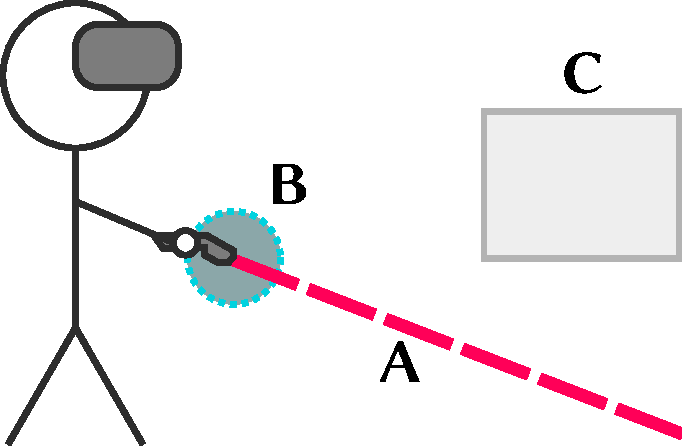
\includegraphics[width=\linewidth]{figures/laserpointer_sketch_no_hit}
        \caption{}
        \label{sfig:laserpointer_sketch_no_hit}
    \end{subfigure}
    \hfill
    \begin{subfigure}{0.45\linewidth}
        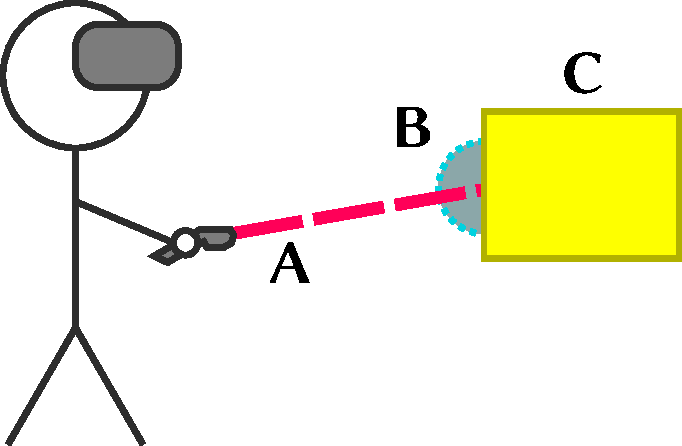
\includegraphics[width=\linewidth]{figures/laserpointer_sketch_hit}
        \caption{}
        \label{sfig:laserpointer_sketch_hit}
    \end{subfigure}
    }
    \caption{Funktionsweise des Laserpointers. %
        Die \lstinline|HoverSphere| wird verschoben, sodass der Raum auf den Vive-Controller reagiert. %
        \textbf{A:} Laserpointer. \textbf{B:} SteamVR-\lstinline|HoverSphere|. \textbf{C:} Auswählbarer Raum.}
    \label{fig:laserpointer_sketch}
\end{figure}

%
\cleardoublepage

\chapter{Nutzerstudie}
\label{chap:evaluation}
\todo{Fragebögen, Flyer, Infobögen etc. in Anhang.}
Wie bereits in \autoref{chap:related_work} erwähnt ist ein Nachteil von 2D-Karten, dass durch das Fehlen einer Dimension zum Abgleich mit der Umgebung ein gewisser mentaler Aufwand notwendig ist.
Die 2D-Karte stellt eine Abstraktion der Umgebung dar, wodurch Informationen verloren gehen.

Der Zweck dieser Nutzerstudie ist zu überprüfen, ob sich bei den Probanden durch die 3D-Megamap ein räumliches Verständnis aufbaut, welches gegenüber der 2D-Karte zu einer performanteren und effizienteren Orientierung führt.
Unter Performanz und Effizienz wird in diesem Sinne verstanden, dass die Fehlerquote und die Zeit zum Einschätzen von Richtungen zu Orten in der Umgebung niedriger sind, als bei der 2D-Variante.
Zudem sollen die subjektiven Eindrücke und Präferenzen der Probanden von den unterschiedlichen Kartenvarianten ermittelt werden.
Für zukünftige Arbeiten werden außerdem Verbesserungsvorschläge und Ansichten über das Potential der Megamap gesammelt.

\section{Aufbau}
Das Experiment wurde im Laborraum 5220 (MZH Ebene 5) der Arbeitsgruppe Human-Computer Interaction an der Universität Bremen durchgeführt.
Für die Präsentation der virtuellen Umgebung wurde die HTC Vive mit zwei Basisstationen eingesetzt.
Der getrackte Bereich zwischen den Basisstationen umfasste ca. \SIrange{0}{0}{\metre}.\todo{Tatsächliche Zahlen einsetzen.}
Die Bilddaten wurden von einem PC mit einer \emph{NVidia~GTX~1080~Ti} Grafikkarte und einem \emph{AMD~Ryzen~7~1800X} Prozessor gerendert.
Übertragen wurden die Bilddaten an das HMD mit dem \emph{VIVE~Wireless~Adapter} \parencite{HTCCorporation2018b}.
Die Fragebögen wurden über \emph{Google Forms} erstellt und ausgefüllt (siehe \autoref{appendix:study_material}).
Hierfür wurde ein separater Laptop bereitgestellt.

\section{Konditionen und Aufgaben}
\label{sec:conditions_and_tasks}
Für die Nutzerstudie wurden drei unterschiedliche Konditionen getestet:
\begin{itemize}
    \item $3D_l$ (\emph{low)}: Die 3D-Megamap wird mit einer Skalierung von \SI{6}{\percent} (relativ zur Umgebung) und \SI{25}{\cm} über dem Boden angezeigt.
    Diese Kondition entspricht am ehesten der Megamap aus TCTD. 
    \item $3D_h$ (\emph{high}): Die 3D-Megamap wird mit einer Skalierung von \SI{6}{\percent} (relativ zur Umgebung) und \SI{1}{\metre} unterhalb der HMD-Position angezeigt.
    Dabei wird die Höhe nur beim Aufrufen der Karte berechnet.
    Danach bleibt die Höhe fix.
    Diese Kondition wird getestet, um zu ermitteln, wie sich die Höhe der Megamap vom Boden auf die Nutzung auswirkt (insbesondere unter dem Aspekt, dass durch die Darstellung in 3D Verdeckungen durch die Wände der Räume auftreten können).
    \item $2D$: Eine 2D-Karte wird senkrecht an der Wand vor dem Nutzer angezeigt.
    Auch die 2D-Karte hat eine Skalierung von \SI{6}{\percent} (relativ zur Umgebung).
    Die Karte ist so an der Wand platziert, dass sie nicht von anderen Wänden oder der Decke und dem Fußboden geschnitten wird.
\end{itemize}
\todo{Screenshots der Konditionen einfügen.}

Jede Kondition wurde über 6~Iterationen (\emph{Tasks}) $T_0, \dots, T_5$ wiederholt.
\todo{Bild für Megamap Varianten} Dabei wurde in jeder Iteration eine andere Indoor-Karte für die Megamap verwendet, um einen Lerneffekt für die Kartenlayouts zu minimieren.
Damit die Konditionen vergleichbar bleiben, wurde jede Karte einmal jeder Kondition unterzogen.
Das heißt, die Probanden durchliefen insgesamt 18~Iterationen, wobei sechs unterschiedliche Karten jeweils dreimal eingesetzt wurden.
Die Reihenfolge der Iterationen innerhalb einer Kondition war zufällig bestimmt, wobei darauf geachtet wurde, dass bei einem Wechsel der Konditionen die gleiche Karte nicht zweimal aufeinander folgte.

Um die Auswirkungen der jeweiligen Kondition auf die mentale räumliche Vorstellung des Probanden von der Umgebung zu testen, wurden eine Suchaufgabe und eine Richtungsschätzung in den Prototypen integriert.

Für die Suchaufgabe wurden auf der jeweiligen Megamap in sieben räumen Bälle platziert.
Die Probanden mussten dann den Raum suchen, der die meisten Bälle enthält und diesen mit dem VIVE Controller und dem virtuellen Laserpointer auswählen.
Jede Megamap hatte genau einen Zielraum, welcher zufällig zwischen sieben und zehn Bällen enthielt.
Die anderen Räume enthielten mindestens fünf Bälle und garantiert weniger als der Zielraum.
Jede der sechs Indoor-Karten hatte denselben Zielraum in allen drei Konditionen.
Dies wurde entschieden, damit die Karten über Konditionen hinweg vergleichbar bleiben.
Wäre immer ein anderer Zielraum gewählt worden, wäre der Schwierigkeitsgrad des Findens zwischen den Konditionen unter Umständen verschieden gewesen, obwohl die Karte die gleiche wäre.

Für den Fall, dass ein Proband einen falschen Raum auswählt, würde dieser rot eingefärbt werden.
Der Proband müsste dann die Suche nach dem Zielraum fortfahren.
Dieser Fall trat über alle Probanden hinweg außerhalb des Tutorials nur ein einziges Mal auf.

Die Probanden mussten sich anhand der Megamap die Richtung vom virtuellen Laborraum zum Zielraum (horizontal und vertikal zentriert) merken.
Sobald sie den Zielraum auswählten, wurde die Megamap ausgeblendet.
Mit dem virtuellen Laserpointer sollten die Probanden dann möglichst mittig auf den Zielraum \emph{in ihrer Umgebung} zeigen.
Durch Betätigen des Triggers konnte der Laserpointer \enquote{eingefroren} werden, um die Richtung entweder zu korrigieren oder zu akzeptieren.
Wenn die Richtung akzeptiert wurde, startete die nächste Iteration.

Damit die Probanden beim Suchen auf einer Karte immer die gleiche Startposition und Blickrichtung hatten wie in den anderen Konditionen, wurde vor der Suchaufgabe ein \emph{User Setup} implementiert.
Die Probanden mussten sich dabei auf eine festgelegte Zielposition stellen und für zwei Sekunden auf ein Ziel an der Wand schauen.
Die beiden Zielpositionen waren von der jeweiligen Karte abhängig, bleiben jedoch für eine Karte über die Konditionen hinweg gleich.
So wurde sichergestellt, dass die Ausgangsbedingungen für die Suche auf der Karte in jeder Kondition gleich bleiben.

Ebenso wurde das User Setup zwischen der Suche und der Richtungsschätzung implementiert.
Ohne diesen Zwischenschritt hätten die Probanden in den 3D-Konditionen einfach den Laserpointer vom Raum auf der Karte anheben müssen, um die korrekte Richtung zu schätzen.
Durch das User Setup wurde eine Ablenkung erzeugt, welche diesen Vorteil der 3D-Konditionen gegenüber der 2D-Kondition minimieren soll.

\section{Ablauf}
Für einen Test wurden \num{45}~Minuten angesetzt.

Zuerst bekamen die Probanden Hintergrundinformationen zu der Nutzerstudie.
Unter anderem wurde erklärt, dass eine neuartige 3D-Darstellung von Indoor-Karten für MR/VR getestet wird und dass verschiedene Varianten getestet würden.
Mit einem Informationsbogen wurden die Probanden über die Details, den Ablauf sowie die gesammelten Daten der Nutzerstudie aufgeklärt.
Daraufhin unterschrieben die Probanden einen Zustimmungsbogen (siehe \autoref{appendix:study_material}).
Dabei willigten zur Teilnahme an der Studie sowie der Aufzeichnung ihres Blickfelds in der virtuellen Umgebung ein.
Die Probanden konnten frei entscheiden, ob zusätzlich eine Audioaufnahme der Gespräche während des Experiments aufgezeichnet wird.

Vor dem eigentlichen Test füllten die Probanden einen allgemeinen Fragebogen aus (siehe \autoref{appendix:study_material}).
Dieser enthielt Fragen zur Person (Alter, Geschlecht usw.) sowie Vorerfahrungen in VR/MR und mit Kartenanwendungen für Außen- und Innenbereiche. Der letzte Teil des Fragebogens ist die ins Deutsche übersetzte Santa~Barbara~Sense-of-Direction~Scale \parencite{Hegarty2002}, mit dem Probanden Selbstauskunft über ihren Orientierungssinn geben.
Die Bewertung wurde von einer 7-Punkte- auf eine 5-Punkte-Likert-Skala abgeändert, um mit den späteren Fragebögen einheitlich zu sein.

Den Probanden wurde danach das VR-Equipment (HMD und Batteriepack für den Wireless~Adapter) angelegt.
Sie fanden sich im virtuellen Laborraum wieder.
Die Probanden wurden kurz in der Bedienung des VIVE Controllers und der Bewegung im Raum innerhalb der Play Area unterrichtet.
Sie wurden darauf hingewiesen, dass an einer der Wände ein Bildschirm hängt, der ihnen den nächsten Aufgabenschritt in Textform anzeigt, sollten sie den Ablauf vergessen.
Die Probanden konnten auch jederzeit während des Experiments Fragen an den Versuchsleiter stellen.

Es folgte ein Tutorial, bei dem die Probanden die zuvor beschriebenen Aufgaben (User~Setup --- Suche --- User~Setup --- Zeigen) in einer Tutorialkondition durchliefen (\SI{40}{\cm} Kartenhöhe vom Boden bei \SI{4}{\percent} Skalierung).
Zuerst wurde die 3D-Megamap gezeigt, danach die 2D-Kondition.
Die Probanden konnten entscheiden, ob sie das Tutorial wiederholen oder fortfahren wollen.
Zu diesem Zeitpunkt wurde die Bildschirmaufnahme (und ggf. die Audioaufnahme) gestartet.

Nach dem Tutorial durchliefen die Probanden die Konditionen und Aufgaben, wie sie in \autoref{sec:conditions_and_tasks} beschrieben sind.
Nach jeder Kondition setzten die Probanden das HMD ab und füllten am Laptop einen Fragebogen zur zuletzt gestesteten Kartenvariante aus (siehe \autoref{appendix:study_material}).
Die Fragebögen basieren auf der \emph{System~Usability~Scale}, wurden jedoch für das Anwendungsgebiet von Karten angepasst.
Die Bewertung der einzelnen Aussagen erfolgte über eine 5-Punkte-Likert-Skala.

Nach Abschluss des letzten Fragebogens wurde mit den Probanden ein kurzes (5--10 Minuten) Leitfadeninterview geführt.
Unter anderem beantworteten die Probanden Fragen zu ihrer präferierten Kartenvariante fürs Suchen und Richtungsschätzen, ihr Vorgehen beim Suchen sowie Verbesserungsvorschlägen.
Die Probanden wurden auch befragt, ob sie sich einen Einsatz von 3D-Megamaps mit MR-HMDs in der realen Welt sowohl in Innen- als auch Außenbereichen vorstellen können.

\section{Testgruppe}
An der Nutzerstudie nahmen 15~Personen teil ($user\_0, \dots, user\_14$), davon 10~männlich und 5~weiblich.
Die Probanden befanden sich in einem Altersbereich von ?? bis ?? Jahren.
Vier der Probanden sind Brillenträger von denen zwei die Brille aus Bequemlichkeitsgründen während des Tests abnahmen.
Zwei der Probanden sprachen Englisch und füllten ins Englische übersetzte Versionen der Fragebögen aus.
Die Muttersprache aller anderen Probanden ist Deutsch.
Keiner der Probanden war in die Inhalte der Masterarbeit oder der Nutzerstudie eingeweiht.

Die Probanden wurden durch an der Universität ausgehängte Flyer (siehe \autoref{appendix:study_material}), den Mailverteiler des Fachbereichs~3 und über die Arbeitsgruppe Human-Computer~Interaction rekrutiert.
Einige Probanden wurden außerdem durch persönlichen Kontakt mit dem Versuchsleiter angeworben.
Für die Teilnahme wurden den Probanden Snacks und Getränke angeboten.
Eine finanzielle Aufwandsentschädigung gab es nicht.

Bei $user_4$ kam es während der ersten Kondition ($3D_h$) zu einem PC-Absturz, der aus einer Inkompatibilität zwischen dem Ryzen-Prozessor und dem VIVE Wireless Adapter resultiert \parencite{HTCCorporation2018c}.
Auch bei einem erneuten Start des Experiments kam es in der Kondition $3D_h$ zum Absturz.
Daraufhin wurde der Test abgebrochen.
Der Proband erschien wenige Tage später und führte das Experiment erneut ohne Absturz durch.
Es wird darauf hingewiesen, dass dieser Nutzer durch die vorige begrenzte Teilnahme für seinen Durchlauf mehr Vorkenntnisse hatte, als die anderen Probanden.

\section{Datenerhebung}
Neben den Antworten aus den Fragebögen wird das Sichtfeld der Proband in der virtuellen Welt aufgezeichnet (und ggf. eine Audioaufnahme des Gesagten).

Zum Vergleich der Performanz von 2D und 3D wird beim Richtungsschätzen die horizontale und vertikale Abweichung von der \enquote{korrekten} Richtung berechnet.
Als korrekte Richtung gilt der Vektor von der Controllerspitze zum Zentrum des Zielraums in der Umgebung.
Die horizontale und vertikale Abweichung ergeben sich aus den jeweiligen Winkeln zwischen der vom Probanden bestätigten Richtung und der korrekten Richtung.

Zum Vergleich der Effizienz werden diverse Zeitmessungen durchgeführt.
Zum einen wird die Zeit gemessen, die Probanden zum Finden des Zielraums benötigen.
Zum anderen wird die Zeit gemessen, bis Probanden die geschätzte Richtung bestätigt haben.
So sollen Aussagen über die Zuversicht der Probanden ihrer Schätzung getroffen werden.

Darüber hinaus werden kontinuierlich die Positionen und Rotationen des HMDs und des Controllers aufgezeichnet.

\section{Ergebnisse}


\subsection{Santa-Barbara Sense-of-Direction Skala}
Vor dem eigentlichen Test füllten Probanden einen Fragebogen nach der SBSOD Skala aus.
Dieser liefert eine Wertung des vom Probanden selbst wahrgenommenen Orientierungssinn.
Zur Auswertung werden die positiv formulierten Elemente invertiert bewertet.
Anschließend wird der Mittelwert über die individuellen Bewertungen berechnet.
Der Mittelwert entspricht der SBSOD-Wertung \parencite{Hegarty2002}.
\autoref{fig:sbsod} stellt das Ergebnis grafisch dar.
Von den 14 Probanden erreichten 12 (\SI{85,71}{\percent}) einen Wert über 3 (\enquote{neutral}).
Im Schnitt wurde eine Bewertung von 3,38 ($\pm$ 0,41) erzielt.
Der höchste erreichte Wert ist 4,07, der niedrigste Wert ist 2,67.
\begin{figure}
    \centering
    \includegraphics[trim={2cm, 0, 2cm, 0}, clip, width=\linewidth]{figures/analysis/sbsod}
    \caption{text}
    \label{fig:sbsod}
\end{figure}

\subsection{Effektivität und Effizienz bei Raumsuche}
\subsubsection*{Suchzeit}
\label{ssec:searchtime}

\begin{table}
    \centering
    \caption{Mittelwert $\mu$ und Standardabweichung $\sigma$ der Suchzeit über alle Karten je Kondition.}
    \label{tab:searchtime_overview}
    \begin{tabular}{rccc}
        \toprule
        {} & \multicolumn{3}{c}{Suchzeit [\SI{}{\second}]} \\
        {} &          $3D_l$ &          $3D_h$ &          $2D$ \\
        \midrule
        $\mu$    &  $\num{27.44}$     &  $\num{28.84}$     &  $\num{18.31}$ \\
        $\sigma$ &  $\pm \num{13.39}$ &  $\pm \num{10.08}$ &   $\pm \num{9.3}$ \\
        \bottomrule
    \end{tabular}
\end{table}

\autoref{tab:searchtime_overview} zeigt eine Übersicht der Suchzeit nach den Zielräumen zwischen den einzelnen Konditionen.
Da die Stichprobenverteilungen der beobachteten Zeiten nicht-normalverteilt ist (wie in \autoref{fig:searchtime_distributions} zu sehen ist), werden nicht-parametrisierte Tests zur Bestimmung der Signifikanz angewendet.
Zwischen den drei Konditionen ist nach dem Friedman-Test ein signifikanter Unterschied festzustellen ($\chi^2(2) = \num{63.5}, p < 0.001$).
Ein paarweiser Wilcoxon-Vorzeichen-Rang-Test zwischen den einzelnen Konditionen zeigt, dass die Suche nach dem Zielraum in $2D$ ($\num{18.31} \pm \SI{9.3}{\second}$) signifikant schneller ist als in $3D_l$ ($\num{27.44} \pm \SI{13.39}{\second}, z=\num{-6.003}, p<\num{0.001}$) und $3D_h$ ($\num{28.84} \pm \SI{10.08}{\second}, z=\num{-7.136}, p<0.001$).
Der Unterschied bei der Suchzeit zwischen $3D_l$ und $3D_h$ ist jedoch nicht signifikant.
\begin{figure}
    \centering
    \includegraphics[width=\linewidth]{figures/analysis/searchtime_distributions}
    \caption{Stichprobenverteilung der beobachteten Suchzeit.}
    \label{fig:searchtime_distributions}
\end{figure}

Weiterhin stellt sich die Frage, ob ein \enquote{besserer} Orientierungssinn zu einer besseren Suchzeit führt.
\autoref{fig:correlation_time_sbsod} zeigt die durchschnittliche Suchzeit der Probanden in Bezug zu den ermittelten SBSOD-Werten aus \autoref{fig:sbsod}.
Für jede Kondition wird Spearmans Rangkorrelationskoeffizient zwischen der SBSOD-Wertung und der durchschnittlichen Suchzeit ermittel.
Die Tests weisen keinen signifikanten Zusammenhang der Variablen aus.
Probanden, die ihren Orientierungssinn besser einschätzen, sind demnach nicht zwingend schneller bei der Suche nach den Zielräumen.
\begin{figure}
    \centering
    \includegraphics[width=\linewidth]{figures/analysis/correlation_time_sbsod_scatter}
    \caption{Scatterplot zur Überprüfung der Korrelation zwischen SBSOD Wertung und Suchzeit.}
    \label{fig:correlation_time_sbsod}
\end{figure}

\subsubsection*{Fehlerrate bei Raumauswahl}
Neben der Suchzeit wurde auch die Zahl der falsch ausgewählten Räume (die Nicht-Zielräume) gemessen.
Über die insgesamt 252 Suchaufgaben (14~Probanden $\times$ 3~Konditionen $\times$ 6~Karten) wurden in drei Fällen (\SI{1,19}{\percent}) vor dem Zielraum falsche Räume ausgewählt.
\autoref{tab:error_searching} zeigt eine Übersicht der entsprechenden Events.
Die Fehler treten jeweils in der ersten Kondition der getesteten Sequenz auf (jedoch nicht in der ersten Karte).
\begin{table}
    \centering
    \caption{Übersicht der Anzahl der falsch ausgewählten Räume währen der Suchaufgabe.}
    \label{tab:error_searching}
    \begin{tabular}{rccccc}\toprule
        Proband                  & Kondition               & Karte    & Suchzeit [\SI{}{\second}] & \# Fehler & Sequenz  \\\midrule
        user\_8                  & $3D_h$                  & Karte\_6 & $\SI{40,61}{\second}$     & 2         & $3D_h$--$3D_l$--$2D$ \\
        user\_9                  & $2D$                    & Karte\_5 & $\SI{38,4}{\second}$      & 1         & $2D$--$3D_l$--$3D_h$ \\\bottomrule
    \end{tabular}
\end{table}

\subsection{Performance und Effizient bei Richtungsschätzung}
\subsubsection*{Genauigkeit der Schätzung}
\autoref{fig:horizontal_offset} zeigt das Ergebnis der Richtungsschätzung.
Da die Abweichung sowohl in positiven Winkeln (Abweichung nach rechts) als auch negativen Winkeln (Abweichung nach links) gemessen wurde, werden hier die absoluten Werte der Abweichung analysiert.
Andernfalls würden die Werte sich bei der Mittelwertbildung gegenseitig aufheben.
Wie zu erkennen ist, liegen die Mittelwerte von $3D_l$~(7,79 $\pm$ \ang{7,22}), $3D_h$~(7,84 $\pm$ \ang{7,44}) und $2D$~(6,62 $\pm$ \ang{5,28}) nahe beieinander.
Der Friedman-Test kann keine signifikanten Unterschiede zwischen den Konditionen nachweisen.
\begin{figure}
    \centering
    \includegraphics[height=0.45\textheight]{figures/analysis/horizontal_offset}
    \caption{Horizontale Abweichung in $\degree$ (Grad) bei der Richtungsschätzung von der tatsächlichen Linie zur Raummitte (ohne vertikale Abweichung).}
    \label{fig:horizontal_offset}
\end{figure}

Ein wesentlicher Aspekt, der die Genauigkeit der Schätzung beeinflusst, ist die Position des Zielraums auf der jeweiligen Karte.
\autoref{tab:herror_per_map} fasst die Mittelwerte und Standardabweichungen der absoluten horizontalen Abweichungen der einzelnen Karten zusammen.
\autoref{fig:horizontal_offset_per_map} zeigt die Unterschiede zwischen den Karten grafisch.
Es ist zu erkennen, dass vor allem die Abweichungen bei Karte 3 und 4 größer sind, als auf den anderen Karten.
Der Friedman-Test bestätigt signifikante Unterschiede zwischen den Karten ($\chi^2(6) = \num{39.755}, p < \num{0.001}$).
Die horizontale Abweichung bei Karte~3 ist signifikant größer als bei Karte~1 ($z = \num{-4,483}, p < \num{0,001}$), Karte~2 ($z = \num{-4,195}, p < \num{0,001}$), Karte~5 ($z = \num{-3,432}, p < \num{0,001}$) und Karte~6 ($z = \num{-3,37}, p < \num{0,001}$).
Auch die hohe Abweichung bei Karte~4 ist gegenüber Karte~1 ($z = \num{-3,782}, p < \num{0,001}$), Karte~2 ($z = \num{-3,395}, p < \num{0,001}$), Karte~5 ($z = \num{-2,044}, p < \num{0,05}$) und Karte~6 ($z = \num{-2,17}, p < \num{0,05}$) signifikant.
Weiterhin gibt es bei Karte~5 eine signifikant größere Abweichung als bei Karte~1 ($z = \num{-2,645}, p < \num{0,008}$), was durch die Ausreißer (siehe \autoref{fig:horizontal_offset_per_map}) begünstigt wird.
\begin{figure}[h!]
    \centering
    \includegraphics[width=0.75\linewidth]{figures/analysis/horizontal_offset_per_map}
    \caption{Absolute horizontale Abweichung in $\degree$ (Grad) bei der Richtungsschätzung pro Karte.}
    \label{fig:horizontal_offset_per_map}
\end{figure}%

\begin{table}[h!]
    \centering
    \caption{Mittelwert $\mu$ und Standardabweichung der absoluten horizontalen Abweichung pro Karte in $\degree$.}
    \label{tab:herror_per_map}
    \begin{tabular}{cccccc}\toprule
        Karte 1 & Karte 2 & Karte 3 & Karte 4 & Karte 5 & Karte 6 \\\midrule
        $\mu = \ang{4,44}$ & $\mu = \ang{4,96}$ & $\mu = \ang{11,75}$ & $\mu = \ang{10,19}$ & $\mu = \ang{6,62}$ & $\mu = \ang{6,55}$ \\
        $\pm \ang{4,03}$ & $\pm \ang{3,3}$ & $\pm \ang{6,98}$ & $\pm \ang{9,07}$ & $\pm \ang{4,94}$ & $\pm \ang{7,05}$ \\\bottomrule
    \end{tabular}
\end{table}

Wird der Unterschied zwischen der positiven und negativen horizontalen Abweichung mit einbezogen, ist eine Tendenz zu einem Ausschlag nach links (negativ) der horizontalen Abweichungen zu erkennen.
Von den insgesamt 252~Richtungsschätzungen weichen 158 (\SI{62,7}{\percent}) nach links ab.

\subsubsection*{Schätzungszeit}
Neben der Abweichung der Schätzung wurde auch die Zeit gemessen, welche die Probanden für die Abgabe der Schätzung benötigen.
\autoref{fig:pointing_time} visualisiert die erhobenen Daten.
In den meisten Iterationen (\SI{95,24}{\percent}) wurde die Richtungsschätzung innerhalb von 10~Sekunden bestätigt.

% TODO: Und weiter???

\begin{figure}
    \centering
    \includegraphics[width=\linewidth]{figures/analysis/pointing_time}
    \caption{Vergleich der Zeit (zwischen den Konditionen), die die Probanden für die Abgabe einer Richtungsschätzung benötigten.}
    \label{fig:pointing_time}
\end{figure}

Einer der Gründe für die Messung der Schätzzeit war es, die Korrelation zur resultierenden horizontalen Abweichung zu testen.
Die Überlegung ist, dass Probanden, die sich mehr Zeit für die Schätzung der Richtung nehmen, präziser sind.
\autoref{fig:pointing_time_vs_error} zeigt die absolute horizontale Abweichung in Bezug zur benötigten Schätzzeit.
Weder grafisch, noch doch Anwendung des Spearman-Tests, ist eine Korrelation zwischen den beiden Variablen erkennbar.
Da die meisten Probanden ihre Schätzung innerhalb der ersten 10~Sekunden abgegeben haben, sind für den Zeitraum \emph{nach} 10~Sekunden zu wenig Messungen vorhanden, um eine zuverlässige Aussage über eine potentielle Korrelation treffen zu können.
\begin{figure}
    \centering
    \includegraphics[width=\linewidth]{figures/analysis/pointing_time_vs_error}
    \caption{Plot der Schätzungszeit gegen die absolute horizontale Abweichung. %
    Eine Korrelation ist nicht erkennbar.}
    \label{fig:pointing_time_vs_error}
\end{figure}

\subsection{Fragebögen zur Nutzungsfreundlichkeit}

\begin{figure}
    \centering
    \includegraphics[width=\linewidth]{figures/analysis/usability}
    \caption{text}
    \label{fig:usability}
\end{figure}

\subsection{Präferenz der Probanden aus Interview}

\section{Diskussion der Ergebnisse}

%
\cleardoublepage

\chapter{Fazit}
\label{chap:closing}
% TODO: Forschungsfrage nochmal aufgreifen?
Die digitale Unterstützung der Navigation und Exploration durch augmentierte Inhalte ist ein Thema, das in der Vergangenheit bereits ausgiebig von Forschung und Industrie behandelt wurde.
Die Idee, eine augmentierte Karte als Megamap in die Umgebung der Nutzer zu integrieren, ist jedoch bisher nur aus Videospielen wie z.B. Tom Clancy's The Division bekannt.
In der vorliegenden Masterarbeit wurde eingehend untersucht, ob sich eine solche Megamap auch für die \enquote{reale} Welt umsetzen lässt.
Zu diesem Zweck wurde das Konzept einer Megamap für den Einsatz mit einem Mixed-Reality-HMD entwickelt.
Mit der Megamap sollen virtuelle Gebäudekarten in das reale Umfeld der Nutzer projiziert werden, sodass diese sich einen Überblick der Umgebung verschaffen können.
Verschiedene explorative Interaktionselemente aus bereits existierenden Kartenanwendungen sind in das Konzept mit eingeflossen und wurden für den Einsatz in Innenbereichen neu interpretiert.
Auf Basis dieses Konzepts wurde ein erster Prototyp der Megamap für die HTC~Vive entwickelt.
In einer Nutzerstudie ($N=15$) wurde mit dem Prototyp die Nutzbarkeit, Effektivität und Effizienz der Megamap für die Suche nach Objekten und den Aufbau einer räumlichen Vorstellung der Umgebung untersucht.
Die Megamap wurde in zwei Varianten getestet (Fußboden- und Bauchhöhe).
Als Vergleichsbasis diente hierzu eine herkömmliche 2D-Darstellung der Gebäudekarten.
Die statistische Analyse der quantitativ erhobenen Daten ergab keine Vorteile der Megamap gegenüber der 2D-Variante in Bezug auf Effektivität oder Effizienz.
Weiterhin bewerteten die Probanden die Nutzbarkeit der 2D-Alternative besser als die der Megamap.
In einem kurzen Leitfadeninterview wurden zudem die subjektiven Meinungen der Probanden zu der Megamap eingeholt.

\section{Probleme des Megamap-Prototypen}
Durch die Nutzerstudie, den Interviews sowie den Erfahrungen bei der Implementierung offenbaren sich drei Probleme des aktuellen Megamap-Prototypen.
Dadurch ergeben sich Ansatzpunkte für zukünftige Verbesserungen und Erweiterungen der Megamap.

\subsection*{Fehlende Suchfunktion und andere Explorationselemente}
Der Hauptgrund für den großen Zeitunterschied zwischen der 2D-Karte und den 3D-Megamaps (siehe \autoref{ssec:searchtime}) ist das Fehlen einer Suchfunktion.
Herkömmliche Kartenapplikationen, wie z.B. die in \autoref{chap:concept} analysierten Webanwendungen, verfügen über eine Suchfunktion für eine spezifische und/oder offene Suche nach Zielorten.
Eine manuelle Suche auf der Karte nach Zielen ist daher nicht notwendig.
In der Nutzerstudie war jedoch die manuelle Suche nach Zielen auf der Karte gefordert.
Dies begünstigt die 2D-Variante, da im Gegensatz zur 3D-Megamap alle Ziel gleichzeitig von den Probanden zu sehen waren.
Dieser Unterschied könnte durch das Implementieren einer Suchfunktion für die Megamap ausgeglichen werden.

Aber auch andere Explorationselemente fehlen im Prototypen.
Das Megamap-Konzept aus \autoref{chap:concept} sieht eine Reihe von Elementen vor, die im aktuellen Prototypen nicht umgesetzt sind.
Dieser wurde mit dem Fokus auf die Aufgabenstellung der Nutzerstudie entwickelt und stellt somit lediglich eine begrenzte Realisierung des eigentlichen Konzepts dar.
Die eigentliche Kartenfunktionalität kommt dabei zu kurz.
Insofern ist die konkrete Implementierung nur teilweise repräsentativ zur Beantwortung der Forschungsfrage dieser Masterarbeit.
Gleichzeitig bedeutet dies aber auch, dass das Potential der Megamap bei Weitem nicht ausgeschöpft ist und das Konzept der Megamap für zukünftige Arbeiten weiterhin interessant bleibt.

\subsection*{Limitierung auf VR-Hardware}
Der vorliegende Prototyp wurde für ein VR-HMD entwickelt, da das gewünschte MR-HMD (Magic Leap One) für die Implementierung nicht zur Verfügung stand.
Wie im vorigen Punkt schränkt auch dies die Repräsentativität des Prototypen für eine Anwendung in MR weiter ein.
Zwar wurde dieses Problem in der Nutzerstudie durch eine virtuelle 1:1-Nachbildung der Umgebung sowie die Verwendung eines Wireless-Adapters adressiert.
Jedoch werden für die VR-Implementierungen Annahmen getroffen, die in einer MR-Anwendung nicht unbedingt gelten.
Beispielsweise ist nicht sicher, ob die Präzision der 3D-Rekonstruktion der MR-HMDs ausreicht, um die Megamap zuverlässig in der Umgebung zu platzieren.
Gleiches gilt für die Berechnung von Schnittpunkten zwischen der Megamap und Objekten in der Umgebung.
Zudem ist die aktuelle Position der Nutzer in der virtuellen Umgebung implizit gegeben.
Für eine MR-Anwendung muss jedoch eine separate Lokalisierung durchgeführt werden, was (je nach Ansatz) zusätzliche Abweichungen in das System einbringen kann.
Diese Probleme müssen für einen zukünftigen Einsatz der Megamap in MR-Anwendungen gelöst werden.

\subsection*{Beschaffung der Indoor-Kartendaten}


\section{Ausblick}
% TODO: Ausblick auf Multi-Stockwerk (Rückreferenz auf ...), Outdoor-MR-Megamap, 
% Technische Neuerungen im Bereich AR (und Anderes)
% ==> Tellerrand!

%
\cleardoublepage


\printbibliography[heading=bibintoc, nottype=online]
\printbibliography[heading=bibintoc, title={Online Referenzen}, type=online]

\end{document}
